\documentclass[a4paper,12pt]{article}

\usepackage{cmap}
\usepackage[T2A]{fontenc}
\usepackage[utf8]{inputenc}
\usepackage[english,russian]{babel}

\usepackage{amsmath, amssymb, amsthm}

\usepackage{indentfirst} %Красная строка
\usepackage[a4paper,top=1.3cm,bottom=2cm,left=1.5cm,right=1.5cm,marginparwidth=0.75cm]{geometry}
\usepackage{hyperref}
\hypersetup{hidelinks}

\usepackage{graphicx}
\graphicspath{{images/}}

\renewcommand{\phi}{\varphi}
\renewcommand{\epsilon}{\varepsilon}

\usepackage{xcolor}

\newtheorem{theorem}{Теорема}[section]
\newtheorem{lemma}{Лемма}[section]
\newtheorem{definition}{Определение}[section]
\newtheorem*{note}{Замечание}

\counterwithin{equation}{section}
\counterwithin{figure}{section}

\renewcommand{\b}{\mathbf}
\renewcommand{\div}{\, \text{div} \,}
\newcommand{\rot}{\, \text{rot} \,}
\newcommand{\h}{\hbar}

\title{Билеты к ГКЭ по общей физике}
\author{Николай Чусовитин}
\date{2021-2022 учебный год}

\begin{document}

\maketitle

\section*{Предисловие}

Данный документ содержит в себе материалы для подготовки к ГКЭ по общей физике на основе экзаменационной программы 2021-2022 года. При составлении использовались в основном учебники Д.В. Сивухина и Н.А. Кириченко. Раздел, посвящённый квантовой физике, написан в основном с использованием лекционного курса В. Н. Глазкова.

Поскольку документ составлялся в течение длительного времени с большими перерывами, стиль и подробность повествования и оформления могут меняться от части к части. Тем не менее, он содержит теоретический минимум по каждому вопросу программы, а зачастую чуть больше, чем минимум.

For aerospace bot squadron with love.

\newpage

\tableofcontents

\newpage
\part{Механика}

\section{Законы Ньютона. Движение тел в инерциальных и неинерциальных системах отсчета.}

\begin{definition}
    Масса (количество материи) есть характеристика тела, являющаяся мерой инерции.
\end{definition}

\begin{definition}
    Импульс (количество движения) есть произведение массы тела на его скорость: $\b p = m \b v$.
\end{definition}

\begin{definition}
    Взаимодействие сил определяется силой $\b F$, которая необходима для изменения состояния покоя или равномерного движения тела.
\end{definition}

\section*{Первый закон Ньютона}

\textit{Существуют системы отсчёта, называемые инерциальными, в которых тела (материальные точки), на которые внешние силы не действуют, или их действие скомпенсировано, покоятся или движутся равномерно прямолинейно.}

\begin{note}
    Инерциальные системы отсчёта движутся равномерно прямолинейно друг относительно друга.
\end{note}

\section*{Второй закон Ньютона}

\textit{В инерциальных системах отсчёта изменение импульса тела прямо пропорционально величине приложенной силы.}

\begin{equation} \label{eq:второй-закон-ньютона-в-импульсной-форме}
    \dot{\b p} = \b F
\end{equation}

Если же движение тела не является релятивистским, то \eqref{eq:второй-закон-ньютона-в-импульсной-форме} можно представить в виде:

\begin{equation} \label{eq:второй-закон-ньютона}
    m \b a = m \ddot{\b r} = \b F
\end{equation}

\section*{Третий закон Ньютона}

\textit{Силы взаимодействия двух материальных точек равны по величине, противоположно направлены и действуют вдоль прямой, соединяющей эти материальные точки.}

\subsection*{Движение тел в инерциальных системах отсчёта}

В инерциальных системах отсчёта движение тел (материальных точек) описывается законами Ньютона и получается при решении дифференциального уравнения \eqref{eq:второй-закон-ньютона-в-импульсной-форме}.

\subsection*{Движение тел в неинерциальных системах отсчёта}

Как было указано ранее, инерциальные системы отсчёта движутся относительно друга равномерно прямолинейно. Пусть в некоторой ИСО $(O_1)$ уравнение движения тела имеет вид

\begin{equation} \label{eq:уравнение-движения-в-исо}
    m  \b a_\text{абс} = \b F
\end{equation}

Пусть $\b R$ -- радиус-вектор точки $M$ в ИСО $O_1$, $\b R_0$ -- вектор $\b{O_1 O}$, описывающий положение НСО относительно ИСО, а $\b r$ -- радиус вектор точки относительно НСО \ref{fig:нсо}. В таком случае будут верны равенства

\begin{align}
    \b R &= \b R_0 + \b r \\
    \dot{\b R} &= \dot{\b R_0} + \dot{\b r} \\
    \ddot{\b R} &= \ddot{\b R_0} + \ddot{\b r}
\end{align}

\begin{figure}[htbp]
    \centering
    \input{images/1_НСО.pdf_tex}
    \caption{Неинерциальная система отсчёта}
    \label{fig:нсо}
\end{figure}

Рассмотрим сначала поступательно движение НСО. Тогда имеем

\begin{align}
    \b v_\text{абс} &= \b v_\text{отн} + \b v_\text{пер} \\
    \b a_\text{абс} &= \b a_\text{отн} + \b a_\text{пер}
\end{align}

Здесь относительная скорость и ускорение описывают движение точки в НСО, а переносные -- движение НСО относительно ИСО. Подставляя результаты в \eqref{eq:уравнение-движения-в-исо}, получим

\begin{equation}
    m  \b a_\text{отн} = \b F - m \b a_\text{пер}
\end{equation}

Слагаемое $- m \b a_\text{пер}$ называется (поступательной) силой инерции.

Если НСО вращается относительно ИСО со скоростью $\boldsymbol \omega$, то эти выражения усложняются:

\begin{align}
    \b{\dot r} &= \left[ \boldsymbol \omega, \b r \right] + \b{v_\text{отн}} \\
    \b{\ddot r} &= \left[\boldsymbol \epsilon, \b r \right] + \left[ \boldsymbol \omega, \left[ \boldsymbol \omega, \b r \right] \right] + 2 \left[ \boldsymbol \omega, \b{v_\text{отн}} \right] + \b a_\text{отн}
\end{align}

Первые два слагаемых относятся к переносному ускорению, а третье называется Кориолисовым. Соответственно они объединятся в силу инерции и Кориолисову силу.
\newpage
\section{Принцип относительности Галилея и принцип относительности Эйнштейна. Преобразования Лоренца. Инвариантность интервала.}

Рассмотрим задачу о равномерном движении ИСО $S'$ относительно ИСО $S$ (рис. \ref{fig:исо}).

\begin{figure}[htbp]
    \centering
    \input{images/2_ИСО.pdf_tex}
    \caption{Относительно движение ИСО}
    \label{fig:исо}
\end{figure}

Пусть для простоты оси систем отсчёта $X, Y, Z,$ и $X', Y', Z'$ соответственно параллельны друг другу, а $X$ и $X'$ совпадают. Пусть также в начальный момент времени $t = 0$ точки $O$ и $O'$ совпадают, а $\b V$ -- относительная скорость движения $S'$ направлена вдоль оси $X$. Переход к более общему случаю осуществляется с помощью переноса начала отсчёта и поворота координат.

Пусть некоторая точка в момент времени $t$ находится в положении $M$. За это время точка $O'$ сдвинется на $\b V t'$ Для положения имеем

\begin{align}
    \b r &= \b r' + \b V t', & t &= t'
\end{align}

\noindent
В проекции на оси это соотношение запишется следующим образом:

\begin{align} \label{eq:преобразования-галилея}
    x &= x' + V t', & y &= y', & z &= z', & t &= t'
\end{align}

\noindent
Формулы обратного преобразования имеют вид

\begin{align} \label{eq:обратные преобразования галилея}
    x' &= x - V t', & y' &= y, & z' &= z, & t' &= t
\end{align}

\noindent
\eqref{eq:преобразования-галилея} и \eqref{eq:обратные преобразования галилея} представляют собой решение задачи о преобразовании координат при движении одной из систем отсчёта. Они называются преобразованиями Галилея.

\begin{note}
    Расстояние $l = \sqrt{\Delta x^2 + \Delta y^2 + \Delta z^2}$ является инвариантом преобразования Галилея.
\end{note}

\noindent
Продифференцировав, получим

\begin{equation}
    \b{\dot r} = \b{\dot r'} + \b V \Leftrightarrow \b v = \b v' + \b V
\end{equation}

\noindent
Это соотношение представляет собой нерелятивистский закон сложения скоростей. При повторном дифференцировании получим

\begin{equation}
    \b a = \b a'
\end{equation}

Поскольку силы не зависят от системы отсчёта, то уравнения движения системы (второй закон Ньютона) инвариантны относительно преобразований Галилея. Это и есть принцип относительности: уравнения механики инвариантны относительно преобразований Галилея (отличие траекторий есть следствие отличия начальных условиях в разных СО). Иначе его можно сформулировать следующий образом: \textit{Законы природы, определяющие изменения состояния движения механический систем, не зависят от того, к какой из двух инерциальных систем отсчёта, движущихся одна относительно другой прямолинейно и равномерно, они относятся}.

Всё физические явления нельзя разделить на чисто механические и немеханические, поэтому имеет место принцип относительности Эйнштейна: \textit{Законы природы, определяющие изменения состояний физических систем, не зависят от того, к какой из двух инерциальных систем отсчёта, движущихся одна относительно другой прямолинейно и равномерно, они относятся}.

Полученные результаты имеют место в предположении об абсолютности времени и расстояния в разных системах отсчёта, но при возрастании скоростей эти предположения нарушаются. Оказывается, например, что скорость света абсолютна и не зависит от системы отсчёта, что противоречит нерелятивистскому закону сложения скоростей. Вернёмся к рассмотрению задачи о двух ИСО (рис. \ref{fig:исо}). В релятивистском случае имеют место преобразования Лоренца:

\begin{align} \label{eq:преобразования лоренца}
    x &= \frac{x' + V t'}{\sqrt{1 - \frac{V^2}{c^2}}}, & y &= y', & z &= z', & t &= \frac{t' + \frac{V}{c^2}x'}{\sqrt{1 - \frac{V^2}{c^2}}}
\end{align}

\noindent
Обратное преобразование:

\begin{align} \label{eq:обратные преобразования лоренца}
    x' &= \frac{x - V t'}{\sqrt{1 - \frac{V^2}{c^2}}} - V t', & y' &= y, & z' &= z, & t' &= \frac{t - \frac{V}{c^2}x}{\sqrt{1 - \frac{V^2}{c^2}}}
\end{align}

\noindent
Дифференцируя \eqref{eq:преобразования лоренца}, получим

\begin{align}
    dx &= \frac{dx' + V dt'}{\sqrt{1 - \frac{V^2}{c^2}}}, & dy &= dy', & dz &= dz', & dt &= \frac{dt' + \frac{V}{c^2}dx'}{\sqrt{1-\frac{V^2}{c^2}}}
\end{align}

\noindent
Отсюда, во-первых, можно получить формулу преобразования скорости

\begin{align} \label{eq:дифференциал преобразований лоренца}
    v_x &= \frac{dx}{dt} = \frac{v_x' + V}{1 + \frac{v_x'V}{c^2}}, & v_y &= v_y' \frac{\sqrt{1 - \frac{V^2}{c^2}}}{1 + \frac{v_x' V}{c^2}}, & v_z &= v_z' \frac{\sqrt{1 - \frac{V^2}{c^2}}}{1 + \frac{v_x' V}{c^2}}
\end{align}

\noindent
Во-вторых, из этих выражений следует инвариантность интервала -- расстояния между точкам в 4-мерном пространстве Минковского $(t, x, y, z)$, $\Delta S^2 = c^2 \Delta t^2 - \Delta x^2 - \Delta y^2 - \Delta z^2$. Рассмотрим приращение интервала между двумя малыми точками:

\begin{equation}
    ds^2 = c^2dt^2 - dx^2 - dy^2 - dz^2 = [\eqref{eq:дифференциал преобразований лоренца}] = ds'^2
\end{equation}

\noindent
Таким образом, интервал инвариантен относительно преобразований Лоренца.
\newpage
\section{Законы сохранения энергии и импульса в классической механике. Упругие и неупругие столкновения.}

Рассмотрим систему материальных точек. На $j$-ую точки системы действуют силы, которые можно разбить на внешние и внутренние: $\b{\dot p}_i = \b F_i^{(e)} + \b F_i^{(i)}$, где внутренние силы -- силы взаимодействия с другими точками этой системы. В силу третьего закона Ньютона для силы взаимодействия между $j$ и $k$ точками $\b F_{kj} + \b F_{jk} = \b 0$. Таким образом $\b{\dot P} = \sum \b{\dot p}_i = \sum \b F_i^{(e)} = \b F^{(e)}$. Если сумма внешних сил равна нулю (в частности, если система замкнута), то имеет место закон сохранения импульса: \textit{Если сумма сил, действующих на систему, равна нулю, то импульс системы сохраняется}.

Рассмотрим теперь понятия работы и энергии.

\begin{definition}
    Элементарной работой называется скалярное произведение силы $\b F$ на элементарном перемещении $d \b s$:
    \begin{equation} \label{eq:элементарная работа}
        \delta A = \left( \b F, d \b s \right)
    \end{equation}
    Работа на пути -- криволинейный интеграл второго рода 
    \begin{equation} \label{eq:работа на пути}
        A = \int_L \left( \b F, d \b s \right)
    \end{equation}
\end{definition}

\noindent
С учётом второго закона Ньютона, получим

\begin{equation}
    \delta A = \b F \cdot d \b s = \frac{d \b p}{dt} \cdot \b v dt = \b v \cdot d \b p
\end{equation}

\noindent
Вспоминая определение импульса, имеем

\begin{equation}
    \delta A = m (\b v, d \b v) = m v dv \Rightarrow A_{12} = m \int_{v_1}^{v_2} vdv = \frac{m v_2^2}{2} - \frac{m v_1^2}{2}
\end{equation}

\begin{definition}
    Величина $K = \dfrac{m v^2}{2}$ называется кинетической энергией.
\end{definition}

Таким образом, работа равна изменению кинетической энергии. Этот факт обобщается на систему материальных точек с необходимостью учитывать работы всех сил, включая внутренние.

\begin{definition}
    Сила называется консервативной, если её работа на замкнутой траектории равна нулю (если работа не зависит от траектории).
\end{definition}

\begin{definition}
    Сила называет гироскопической, если зависит от скорости точки и действует перпендикулярно ей.
\end{definition}

\begin{note}
    Гироскопические силы не совершают работу.
\end{note}

Если на систему сил действуют только гироскопические и консервативные силы, то можно ввести понятие потенциальной энергии. Выберем <<нулевое>> положение системы, а работу, совершаемую консервативными силами при перемещении в это положение, назовём потенциальной энергией. Потенциальная энергия $U$ является функцией только координат, а консервативные силы $F = - \nabla U$. Работа этих сил при переходе из состояния 1 в состояние 2 равна $A_{12} = U_1 - U_2 = - \Delta U$.

Вспомним, что работа сил равна приращению кинетической энергии. Тогда в консервативной системе имеем

\begin{equation}
    K_2 - K_1 = U_1 - U_2 \Rightarrow K_1 + U_1 = K_2 + U_2 = E = \text{const}
\end{equation}

Величина $E$ называется полной энергией системы. Таким образом, мы получаем закон сохранения энергии: \textit{Полная энергия консервативной системы (с гироскопическими силами) сохраняется}.

Законы сохранения и импульса часто применяются для решения задач о соударениях частиц. Удар называется абсолютно неупругим, если после него два тела <<слипаются>> и продолжают движение вместе. В таком случае закон сохранения импульса даёт

\begin{equation}
    m_1 \b v_1 + m_2 \b v_2 = \left( m_1 + m_2 \right) \b u
\end{equation}

\noindent
а полная механическая энергия системы уменьшается.

Удар называется абсолютно упругим, если механическая энергия системы сохраняется. Для решения задач об упругих ударах необходимо рассматривать системы из уравнений ЗСИ и ЗСЭ.
\newpage
\section{Уравнение движения релятивистской частицы под действием внешней силы. Импульс и энергия релятивистской частицы.}

\begin{definition}
    Импульс релятивистской частицы $\b p = \dfrac{m \b v}{\sqrt{1 - \frac{v^2}{c^2}}}$.
\end{definition}

При таком определении импульса уравнение движения принимает вид

\begin{equation} 
    \frac{d}{dt} \left( \frac{m \b v}{\sqrt{1 - \frac{v^2}{c^2}}} \right) = \b F
\end{equation}

\noindent
С учётом обозначения Лоренц-фактора $\gamma = \dfrac{1}{\sqrt{1 - \frac{v^2}{c^2}}}$, при дифференцировании получим

\begin{equation} \label{eq:уравнение движения релятивистской частицы}
    \b F = \gamma m \frac{d \b v}{dt} + m \b v \left[ \frac{1}{2 \left( 1 - \frac{v^2}{c^2} \right)^{3/2}} \right] \left( \frac{2 \b v}{c^2},  \frac{d \b v}{dt} \right) = \gamma m \b a + \gamma^3 \frac{m}{c^2} \b v \left( \b v, \b a \right)
\end{equation}

\noindent
Таким образом, в общем случае ускорение не параллельно силе. Домножив обе части равенства \eqref{eq:уравнение движения релятивистской частицы} скалярно на $\b v$, получим:

\begin{equation*}
    \left( \b v, \b F \right) = \gamma^3 m \left( \b v, \b a \right)
\end{equation*}

\noindent
Используя это соотношение приведём \eqref{eq:уравнение движения релятивистской частицы} к виду 

\begin{equation}
    \gamma m \b a = \b F - \frac{\b v}{c^2} \left( \b v, \b F  \right)
\end{equation}

Получим выражение для кинетической энергии в случае действия силы вдоль скорости:

\begin{equation}
    \delta A = d K = \left( \b F, d \b s \right) = \left( \b F, \b v dt \right) = \gamma^3 m v dv
\end{equation}

\begin{equation}
    K = \int_0^v \frac{m d \left( v^2 \right)}{2 \left( 1 - \frac{v^2}{c^2} \right)^{3/2}} = \left( \gamma - 1 \right) m c^2
\end{equation}

Величина $E = \gamma m c^2$ называется полной энергией тела, $E_0 = m c^2$ -- энергией покоя, а их разница -- кинетической энергией. С учётом выражения импульса имеем

\begin{equation}
    E^2 = \left( m c^2 \right)^2 + \left( p c \right)^2
\end{equation}

Поскольку энергия покоя инварианта относительно преобразований ЛОренца, то величина $E^2 - \left( p c \right)^2$ также является релятивистским инвариантом. Законы сохранения энергии и импульса остаются верны и в релятивистской механике.
\newpage
\section{Закон всемирного тяготения и законы Кеплера. Движение тел в поле тяготения.}

Кеплер эмпирически установил три закона движения планет, основываясь на результатах многолетних анстрономических наблюдений. Их формулировки выглядят следующим образом:

\begin{enumerate}
    \item \textit{Каждая планета движется по эллипсу, в одном из фокусов которого находится Солнце.}
    \item \textit{Радиус-вектор планеты за равные промежутки времени заметает равные площади.}
    \item \textit{Квадраты времён обращений планет относятся как кубы больших полуосей эллиптических орбит, которые они описывают вокруг солнца.}
\end{enumerate}

На основе этих законов Ньютон получил закон всемирного тяготения:

\begin{equation} \label{eq:закон всемирного тяготения}
    \b F = - G \frac{m_1 m_2}{r^3} \b r
\end{equation}

Покажем вывод второго и третьего законов Кеплера из закона всемирного тяготения. Поскольку сила притяжения центральна, то на тело не действует никаких моментов сил, а значит имеет место закон сохранения момента импульса:

\begin{equation*}
    \b L = \left[ \b r, m \b v \right] = \text{const}
\end{equation*}

\begin{equation*}
    \frac{dS}{dt} = \frac{r v_\phi}{2} = \frac{|\left[ \b r, \b v_\phi \right]|}{2} = \text{const}
\end{equation*}

Введём потенциальную энергию $U = - G \frac{M m}{r}$. Для движения в поле тяжести имеет место закон сохранения энергии:

\begin{equation*}
    \frac{m v^2}{2} - G \frac{M m}{r} = \epsilon = \text{const}
\end{equation*}

\noindent
Рассмотрим крайние точки эллипса. В них скорость имеет только поперечную составляющую. С учётом сохранения момента импульса имеем для них

\begin{equation*}
    \frac{L^2}{2 m r^2} - G \frac{M m}{r} = \epsilon
\end{equation*}

\noindent
Это квадратное уравнение и по теореме Виета сумма его корней равна

\begin{equation*}
    r_1 + r_2 = - G \frac{M m}{\epsilon} = 2a \Rightarrow \epsilon = - G \frac{M m}{2 a}
\end{equation*}

\begin{figure}[htbp]
    \centering
    \input{images/3_эллипс.pdf_tex}
    \caption{Траектория движения тела в поле тяготения}
    \label{fig:эллипс}
\end{figure}

Заметим теперь, что сумма расстояний от фокусов до точки на эллипсе постоянна. Таким образом двойное расстояния от фокуса $2 CB = 2a \Rightarrow CB = a$. Отсюда получим скорость в точке $B$ (рис. \ref{fig:эллипс}):

\begin{equation*}
    \frac{m v_B^2}{2} - G \frac{M m}{a} = \epsilon = - G \frac{M m}{2 a} \Rightarrow v_B = \sqrt{\frac{G M}{a}}
\end{equation*}

\noindent
Наконец, рассчитаем период обращения:

\begin{equation*}
    S = \pi a b = \frac{L}{2 m} T \Rightarrow T = \frac{2 \pi a b m}{L} = \frac{2 \pi a}{v_B} \Rightarrow T^2 \propto a^3
\end{equation*}

\noindent
Что и доказывает третий закон Кеплера.
\newpage
\section{Закон сохранения момента импульса. Уравнение моментов. Вращение твердого тела вокруг неподвижной оси. Гироскопы.}

\begin{definition}
    Моментом силы $\b F$ относительно точки (полюса) $O$ называется векторное произведение $\b M = \left[ \b r, \b F \right]$, где $\b r$ -- радиус-вектор точки приложения силы.
\end{definition}

\begin{definition}
    Моментом импульса материальной точки с импульсом $\b p$ относительно точки (полюса) $O$ называется векторное произведение $\b L = \left[ \b r, \b p \right]$.
\end{definition}

Для производной момента импульса имеем:

\begin{equation*}
    \b{\dot L} = \left[ \b{\dot r}, \b p \right] + \left[ \b r, \b{\dot p} \right]
\end{equation*}

Поскольку при неподвижном начале координат скорость тела параллельна импульсу, то первое слагаемое обращается в ноль. С учётом второго закона Ньютона получаем уравнение моментов:

\begin{equation} \label{eq:уравнение моментов}
    \b{\dot L} = \b M
\end{equation}

Для замкнутой механической системы по аналогии с законом сохранения импульса имеет место закон сохранения момента импульса, поскольку сумма моментов противоположных сил так же равна нулю.

Рассмотрим вращение вокруг неподвижной оси. Если материальная точка вращается вокруг оси $O$ по окружности радиуса $r$ со скоростью $v$, то её момент импульса равен $L = mvr$. Пусть $\omega$ -- угловая скорость точки. Тогда для момента импульса имеет место выражение $L = m r^2 \omega = I \omega$, где величина $I$ называется моментом инерции относительно оси $O$. В случае системы материальных точек (твёрдого тела) момент инерции вычисляется как сумма (интеграл) по всем точкам системы (по всему телу). Отсюда получим основное уравнение динамики вращательного движения относительно неподвижной оси:

\begin{equation}
    \frac{d}{dt}\left( I \omega \right) = M
\end{equation}

Более общим понятием, чем момент инерции, является тензор инерции, в вывод которого углубляться не будем. Заметим лишь, что это симметричный тензор второго ранга, который можно привести к диагональному виду в ОНБ из собственных векторов, причём для твёрдого тела верно

\begin{equation}
    \b L = \hat I \boldsymbol \omega
\end{equation}

\noindent
То есть во общем случае момент импульса не сонаправлен с угловой скоростью.

Рассмотрим динамически-симметричное тело: тело, у которого два главных момента инерции совпадают. В таком теле момент импульса можно представить в следующем виде:

\begin{equation}
    \b L = I_\parallel \boldsymbol \omega_\parallel + I_\perp \boldsymbol \omega_\perp
\end{equation}

\noindent
Пусть составляющая угловой скорости вокруг оси симметрии намного больше, чем другая её составляющая. В таком случае при вычислении момента импульса можно пренебречь вторым слагаемым. Если приложить силу к оси гироскопа, то момент сил будет перпендикулярен моменту импульса, а значит может изменить лишь его направление, а не скорость. При постоянной силе это явление называется вынужденной регулярной прецессией гироскопа. Пусть $\boldsymbol \Omega$ -- скорость прецессии. Тогда имеем

\begin{equation}
    \b{\dot L} = \left[ \boldsymbol \Omega, \b L \right] = \b M = \left[ \b a, \b F \right]
\end{equation}

\noindent
Основная формула гироскопии:

\begin{equation}
    \Omega = \frac{M}{L}
\end{equation}
\noindent
Если же ось гироскопа наклонена относительно оси прецессии, то формула примет вид

\begin{equation}
    \boldsymbol \Omega = - \frac{a}{L} \b F
\end{equation}
\newpage
\section{Течение идеальной жидкости. Уравнение непрерывности. Уравнение Бернулли.}

Движение жидкостей или газов можно рассматривать различными способами. Один из способов -- описание движения каждой отдельно взятой частицы. Другой -- описание параметров течения (скорость, плотность, температура) в каждой точке пространства. При таком подходе параметры жидкости являются функциями координат и времени.

\begin{definition}
    Течение называется стационарным, если его параметры не меняются со временем.
\end{definition}

\begin{definition}
    Жидкость называется идеальной, если при её движении не учитывается трение о стенки и слои жидкости между собой.
\end{definition}

Рассмотрим элемент объема жидкости, не перемещающийся в пространстве. Масса в нём может меняться только за счёт "утекания через стенки":

\begin{equation*}
    \frac{\partial m}{\partial t} = \frac{\partial}{\partial t} \int_V \rho dV = - \oint_{\partial V} \rho \b v \cdot d \b A
\end{equation*}

\noindent
Пользуясь теоремой Гаусса-Остроградского для перехода от поверхностного интеграла к объёмному и равенства нулю этого интеграла по произвольному объёму получим уравнение непрерывности:

\begin{equation} \label{eq:уравнение непрерывности}
    \frac{\partial \rho}{\partial t} + \left( \nabla, \rho \b v \right) = 0
\end{equation}

Аналогом закона Ньютона для идеальной жидкости является уравнение Эйлера. Сила, действующая на малый объём со стороны давления выражается следующим интегралом:

\begin{equation*}
    - \oint_{\partial V} p d \b A
\end{equation*}

\noindent
Или, переходя к объёмному интегралу:

\begin{equation*}
    - \int_V \nabla p dV
\end{equation*}

\noindent
Таким образом для элемента объёма жидкости имеем:

\begin{equation*}
    \rho \frac{d \b v}{dt} = - \nabla p
\end{equation*}

\noindent
Если так же учесть объёмные силы $\b f$ и раскрыть полную производную скорости, получим уравнение Эйлера:

\begin{equation}
    \rho \left( \frac{\partial \b v}{\partial t} + \left( \b v, \nabla \right) \b v \right) = - \nabla p + \rho \b f
\end{equation}

Рассмотрим теперь стационарное течение идеальной жидкости в поле тяжести вдоль линии тока. Градиент в таком случае есть производная по направлению кривой $\frac{\partial}{\partial l}$, а сила тяжести потенциальна и равна градиенту потенциала соответственно. Тогда имеем

\begin{equation*}
    \rho \b v \frac{\partial \b v}{\partial l} = - \frac{\partial p}{\partial l} - \frac{\partial\left( \rho g h \right)}{\partial l}
\end{equation*}

\noindent
Проинтегрировав, получим уравнение Бернулли для идеальной жидкости:

\begin{equation}
    \frac{\rho v^2}{2} + p + \rho g h = \text{const}
\end{equation}
\newpage
\section{Закон вязкого течения жидкости. Формула Пуазейля. Число Рейнольдса, его физический смысл.}

В реальных (неидеальных) жидкостях помимо сил давления действуют касательные силы вязкости. Для получения количественных законов вязкости рассмотрим следующий пример: пусть слой жидкости заключён между двумя бесконечно длинными параллельными пластинками. Нижняя пластинка пусть неподвижна, а верхняя движется относительно неё со скоростью $\b v_0$. Оказывается, что для поддержания равномерного движения верхней пластинки к ней надо будет приложить силу $\b F$ направленную в сторону движения. Такая же сила, противоположная по направлению, должна быть приложена к нижней пластинке для сохранения неподвижности. Ньютоном было установлено, что эта сила пропорциональна площади пластинки $S$, скорости $v_0$, и обратно пропорциональна расстоянию между пластинками $h$:

\begin{equation} \label{eq:закон вязкости ньютона}
    F = \eta S \frac{v_0}{h}
\end{equation}

Постоянная $\eta$ называется вязкостью жидкости и зависит только от жидкости, но не от материала пластинок. Обобщение этой формулы можно получить, разбивая движущуюся жидкость на тонкие слои. Результатом будет формула для касательного напряжения:

\begin{equation}
    \tau_{yx} = \eta \frac{\partial v_x}{\partial y}
\end{equation}

Рассмотрим стационарное течение вязкой несжимаемой жидкости по цилиндрической прямолинейной трубе радиуса $R$. Если выделить бесконечно маленькую трубку тока, то из несжимаемости жидкости будет следовать постоянство скорости на этой линии тока, так что скорость течения $v$ является только функцией радиуса $r$. Рассмотрим теперь тонкий цилиндр жидкости толщины $dx$ и радиуса $r$. На него действует касательная сила вязкости

\begin{equation*}
    2 \pi r \eta \frac{dv}{dr} dx
\end{equation*}

\noindent
Так же на него действует сила разности давлений

\begin{equation*}
    \left( P(x) - P(x + dx) \right) S = - \pi r^2 \frac{dP}{dx} dx
\end{equation*}

\noindent
При стационарном течении скорость постоянна, а значит сумма этих сил должна быть равна нулю:

\begin{equation*}
    2 \eta \frac{dv}{dr} = r \frac{dP}{dx}
\end{equation*}

\noindent
Скорость $v(r)$, а значит и её производная не зависят от $x$, а значит производная $\frac{dP}{dx}$ является постоянной и будет равна

\begin{equation*}
    \frac{dP}{dx} = \frac{P_2 - P_1}{l}
\end{equation*}

\noindent
Где $l$ -- длина трубы, а $P_1$ и $P_2$ -- давления на входе и выходе соответственно. Таким образом получаем формулу

\begin{equation}
    \frac{dv}{dr} = -  \frac{P_1 - P_2}{2 \eta l} r
\end{equation}
\noindent
При интегрировании получим

\begin{equation*}
    v = C - \frac{P_1 - P_2}{4 \eta l} r^2
\end{equation*}

\noindent
Постоянная интегрирования определяется из условия равенства нулю скорости на стенках трубы. Таким образом, скорость вязкой жидкости при удалении от оси меняется по параболическому закону:

\begin{equation}
    v = \frac{P_1 - P_2}{4 \eta l} \left( R^2 - r^2 \right)
\end{equation}

Рассчитаем теперь расход жидкости при таком течении. Масса жидкости, протекающая через кольцо с внутренним радиусом $r$ и внешним $r + dr$ равна $dQ = 2 \pi r dr \cdot \rho v$. Тогда

\begin{equation*}
    Q = \pi \rho \frac{P_1 - P_2}{2 \eta l} \int_0^R \left( R^2 - r^2 \right) r dr
\end{equation*}

\begin{equation} \label{eq:формула Пуазейля}
    Q = \pi \rho \frac{P_1 - P_2}{8 \eta l} R^4
\end{equation}

\noindent
Последняя формула и называется формулой Пуазейля. Заметим, что она верна только для \textit{ламинарных} течений, то есть тех, в которых слои жидкости не перемешиваются между собой и трубки тока параллельны трубе. При больших скоростях ламинарное течение становится турбулентным и формула \eqref{eq:формула Пуазейля} перестаёт быть верной. Тип течения характеризуется числом Рейнольдса

\begin{equation}
    Re = \frac{\rho l v_0}{\eta}
\end{equation}

Число Рейнольдса пропорционально отношению кинетической энергии жидкости к энергии, теряемой из-за вязкости на характерной длине. Оно определяет относительную роль инерции и вязкости жидкости. При больших числах преимущественна инерция, при малых -- вязкость. При больших числах Рейнольдса течение обычно турбулентное, при малых -- ламинарное, однако возможны исключения.
\newpage
\section{Упругие деформации. Модуль Юнга и коэффициент Пуассона. Энергия упругой деформации.}

Все тела деформируемы, то есть меняют форму и объём при приложении внешних сил. Если при прекращении действия приложенных сил деформации исчезают, они называются \textit{упругими}. Иначе -- \textit{пластическими}. Тип деформации зависит не только от материала, но и от прикладываемой силы. Если напряжение (сила на единицу площади) превзойдёт предел упругости, то деформация будет пластичной.

Для определения понятия напряжения рассмотрим деформированное тело или среду. Мысленно разделим его на два и посмотрим на границу раздела. Полученные тела будут взаимодействовать с некоторой силой. Пусть на элемент поверхности одного из них $dS$ действует сила $d \b F$. Тогда напряжением назовём отношение силы к площади:

\begin{equation}
    \boldsymbol \sigma = \frac{d \b F}{dS}
\end{equation}

\noindent
В общем случае напряжённое состояние характеризуется \textit{тензором напряжений}.

Рассмотрим наиболее простой случай: одномерное растяжение/сжатие стержня. Если он растягивается под действием силы $F$, то напряжение будет равно

\begin{equation*}
    \sigma = \frac{F}{S}
\end{equation*}

\noindent
где $S$ -- площадь поперечного сечения стержня. Пусть $l_0$ -- длина недеформированного стержня, а $\Delta l$ -- приращение длины. Тогда вводится понятия относительного удлинения/сжатия (\textit{относительная деформация}):

\begin{equation}
    \epsilon = \frac{\Delta l}{l_0}
\end{equation}

Опыт показывает, что при малых деформациях относительная деформация пропорциональна напряжению

\begin{equation} \label{eq:закон гука}
    \sigma = E \epsilon
\end{equation}

\noindent
Коэффициент пропорциональности $E$ зависит от вещества и называется \textit{модулем Юнга}.

Закон Гука также представим в виде $F = k \Delta x$, где $k = E \frac{S}{l}$. Тогда работа, совершаемая при деформации, равна

\begin{equation}
    U = \int_0^{\Delta l} k x dx = \frac{k \Delta l^2}{2}
\end{equation}

\noindent
В терминах напряжений и относительных деформаций имеем

\begin{equation}
    U = \frac{E S l^2 \epsilon^2}{2 l} = \frac{E \epsilon^2}{2} V
\end{equation}

\noindent
Таким образом, упругая энергия единицы объёма

\begin{equation}
    u = \frac{E \epsilon^2}{2}
\end{equation}

Опыт показывает, что под действием растягивающей или сжимающей силы изменяются не только продольные, но и поперечные размеры. Если сила растягивающая, то поперечные размеры уменьшаются, если сжимающая -- увеличиваются. Коэффициент пропорциональности между поперечной и продольной деформацией называют \textit{коэффициентом Пуассона}:

\begin{equation}
    \mu = - \frac{\epsilon_\perp}{\epsilon_\parallel} = - \frac{\Delta d / d_0}{\Delta l / l_0}
\end{equation}

\noindent
С учётом поперечных деформаций и закона Гука можно получить следующую формулу:

\begin{equation}
    \epsilon_x = \frac{\sigma_x}{E} - \mu \frac{\sigma_y + \sigma_z}{E}
\end{equation}

Модуль Юнга и коэффициент Пуассона полностью характеризуют упругие свойства изотропного материала.
\newpage

\part{Термодинамика и молекулярная физика}

\section{Уравнение состояния идеального газа, его объяснение на основе молекулярно-кинетической теории. Уравнение неидеального газа Ван-дер-Ваальса.}

Системы, рассматриваемые в термодинамике, как например газы, содержат в себе очень большое число частиц, поэтому их описание путем описания, например, траекторий и скоростей всех частиц не представляется возможным. Для описания состояния таких систем используются макроскопические параметры: давление, объём, температура и т.д. Оказывается, что если две макроскопические величины заданы, то они однозначно определяют третью и для таким систем можно записать \textit{уравнение состояния:}

\begin{equation*}
    f(P, V, T) = 0
\end{equation*}

\begin{definition}
    Газ, подчиняющийся законам Бойля-Мариотта ($PV = f(T)$) и Гей-Люссака ($P/T = g(P)$) будем называть идеальным. Эквивалентное определение идеального газа -- газ, в котором не учитывается взаимодействие молекул за исключением соударения.
\end{definition}

Следствием этих экспериментальных законов является уравнение состояния идеального газа, называемое уравнением Менделеева-Клапейрона:

\begin{equation}
    P V = \nu R T
\end{equation}

Получим формулу для давления идеального газа с точки зрения молекулярно-кинетической теории. Разделим молекулы на группы так, что в одной и той же группы молекулы имеют примерно одинаковую по величине и направлению скорость. Скорость молекул этой группы -- $v_i$, а концентрация -- $n_i$. Рассмотрим площадку $\sigma$ на стенке сосуда. Пусть $i$-ые молекулы движутся к ней. За время $dt$ с ней столкнётся $n_i v_{i n} \sigma dt$ молекул, где $v_{in}$ -- нормальная составляющая скорости к площадке.

Рассчитаем силу, с которой эти молекулы давят на площадку. Предположим, что удары абсолютно упругие. Тогда для одной молекулы $dF_i = dp / dt = 2 m v_{in} / dt$, а для всех попадающих на стенку за время $dt$ $F_i = 2 m n_i v_{in}^2 \sigma$, или $P_i = 2 m n_i v_{in}^2$. С учётом равномерного распределения на стенку давит примерно $1/6$ всех молекул, таким образом

\begin{equation*}
    P = \frac{1}{3} m n \overline{v^2}
\end{equation*}

\noindent
или

\begin{equation}
    P V = N m \overline{v^2} = \frac{2}{3} N \overline{E_\text{пост}} = \nu R T
\end{equation}

Однако, модель идеального газа не всегда даёт верные результаты. Из-за взаимодействия между частицами поведение реального газа может значительно отличаться. Одним из уравнений, учитывающих это взаимодействие, является уравнение Ван-дер-Ваальса. Учтём влияние молекулярных сил в уравнении Менделеева-Клапейрона. Во-первых на малых расстояниях молекулы отталкиваются друг от друга, уменьшая доступный объём:

\begin{equation*}
    V \to V - b
\end{equation*}

\noindent
Во-вторых, на больших расстояниях они притягиваются, уменьшая давление:

\begin{equation*}
    P \to P + \frac{a}{V^2}
\end{equation*}

\noindent
Результатом этих предположений является уравнение Ван-дер-Ваальса для одного моля:

\begin{equation}
    \left( P + \frac{a}{V^2} \right) \left( V - b \right) = R T
\end{equation}

\noindent
Или для, нескольких молей:

\begin{equation}
    \left( P + \frac{a \nu^2}{V^2} \right) \left( V - b \nu \right) = \nu R T
\end{equation}
\newpage
\section{Квазистатические процессы. Первое начало термодинамики. Количество теплоты и работа. Внутренняя энергия. Энтальпия.}

\begin{definition}
    Термодинамическое равновесие -- состояние, в которое изолированная система приходит с течением времени и не выходит из него.
\end{definition}

\begin{definition}
    Квазистатические процесс -- процесс, который состоит из непрерывно следующих друг за другом равновесных состояний.
\end{definition}

При расширении или сжатии газ способен совершать работу. Рассмотрим, например, газ под поршнем. Пусть поршень сместился на малое расстояние $dx$, так что давление газа практически не изменилось. Тогда работа, совершённая газом, будет равна $\delta A = F dx = P S dx = P dV$, где $S$ -- площадь поршня. При квазистатическим процессах каждое состояние является равновесным, а значит работа внешних сил равна работе газа, взятой со знаком <<->> : $A_\text{внеш} = - A$.

Введём понятие адиабатической оболочки:

\begin{definition}
    Оболочка называется адиабатической, если состояние системы внутри неё остаётся неизменным при любых изменениях температуры тел вне оболочки.
\end{definition}

Сформулируем первое начало термодинамики для систем в адиабатических оболочках: \textit{Если система тел адиабатически изолирована, то работа внешних сил над этой системой зависит только от конечного и начального состояний этой системы, но не от пути, по которому осуществляется переход.} В рамках этого утверждения можно определить понятие внутренней энергии системы:

\begin{definition}
    Внутренней энергией системы $U$ называется функция состояния, приращение которой равно работе внешних сил, совершаемых над системой в адиабатической оболочке при переходе от одного равновесного состояния к другому.
\end{definition}

\begin{note}
    Внутренняя энергия определена с точностью до аддитивной постоянной.
\end{note}

Если система помещена в адиабатическую оболочку, то единственным способом изменения её внутренней энергии является совершение работы (путём изменения внешних параметров). Однако если адиабатической изоляции нет, то изменение внутренней энергии возможно, например, с помощью теплообмена.

\begin{definition}
    Энергия, полученная телом в результате теплообмена с окружающей средой, называется количеством теплоты или теплотой.
\end{definition}

Теперь можно дать математическую формулировку первого начала термодинамики: \textit{Теплота, полученная системой, идёт на приращение её внутренней энергии и совершение работы.}

\begin{equation}
    Q = \Delta U + A
\end{equation}

\noindent
Для квазистатических процессов

\begin{equation}
    \delta Q = dU + \delta A = dU + P dV
\end{equation}

Далее будет введено понятие энтропии $dS = \delta Q / T$, причём для квазистатических процессов имеет место равенство $dU = T dS - PdV$.

Помимо давления, объёма, температуры, внутренней энергии и т.п. есть ещё множество функций, которые можно использовать для описания термодинамической системы. Введём понятие \textit{энтальпии} $H$ (или $I$):

\begin{equation}
    H = U + PV
\end{equation}

\noindent
Для дифференциала энтальпии имеем:

\begin{equation}
    dH = T dS + V dP
\end{equation}

\textit{Энтальпия есть такая функция состояния, приращение которой в процессе при постоянном давлении равно количеству теплоты, полученному системой.}
\newpage
\section{Второе начало термодинамики. Цикл Карно. Энтропия и закон ее возрастания. Энтропия идеального газа. Статистический смысл энтропии.}

Существует множество различных формулировок второго начала термодинамики. Рассмотрим две классических.

\begin{itemize}
    \item Томсон: \textit{Невозможен круговой процесс, единственным результатом которого является совершение работ за счёт охлаждения теплового резервуара (получения тепла).}
    \item Клаузиус: \textit{Теплота не может самопроизвольно переходить от менее нагретого тела к более нагретому (нельзя передать теплоту так, чтобы в природе не произошло больше никаких изменений).}
\end{itemize}

Покажем эквивалентность этих определений. Пусть процесс Клаузиуса возможен. Тогда возьмём тепловую машину, которая отнимет у нагревателя теплоту $Q_1$ и отдаст холодильнику теплоту $Q_2$, совершив при этом работу $A = Q_1 - Q_2$. С помощью процесса Клаузиуса затем вернём нагревателю теплоту $Q_2$. Тогда мы получили процесс, единственным результатом которого является совершение работы за счёт охлаждения нагревателя, что противоречит невозможности процесса Томсона.

Предположим теперь, что возможен процесс Томсона. Тогда отнимем теплоту $Q$ у менее нагретого тела и с помощью работы в процессе Томсона (например, за счёт трения) передадим её более горячему. Мы получили процесс Клаузиуса. Эквивалентность формулировок доказана.

Рассмотрим процесс Карно, в котором система приводится в тепловой контакт с тепловыми резервуарами, температуры которых равны $T_1$ и $T_2$, $T_1 > T_2$. Более горячий резервуар -- нагреватель, более холодный -- холодильник (охладитель). Цикл Карно состоит в следующем:

\begin{enumerate}
    \item Система, имея температуру $T_1$ приводится в тепловой контакт с нагревателем. При квазистатическом уменьшении давления система изотермически расширяется, забирая теплоту у нагревателя и совершая работу против внешнего давления.
    \item После система адиабатически изолируется и расширяется по адиабате, пока не достигнет температуры $T_2$, также совершая работу.
    \item Система приводится в тепловой контакт с холодильником и изотермически сжимается, отдавая теплоту холодильнику, при этом система совершает отрицательную работу.
    \item Система адиабатически сжимается до температуры $T_1$.
\end{enumerate}

В результате цикла внутренняя энергия системы не меняется, работа есть $A = Q_1 - Q_2$, а КПД соответственно

\begin{equation}
    \eta = \frac{Q_1 - Q_2}{Q_1}
\end{equation}

\begin{theorem}[Первая теорема Карно]
    КПД тепловой машины, работающей по циклу Карно, зависит только от температур нагревателя и холодильника и не зависит от устройства машины или вида рабочего вещества.
\end{theorem}

\begin{proof}
    Рассмотрим две машины Карно, имеющие общие нагреватель и холодильник. Пусть КПД первой -- $\eta$, а второй -- $\eta'$. Предположим, что $\eta > \eta'$.

    Цикл Карно -- квазистатический, а значит его возможно проводить в обратном направлении. Пусть в результате $m$ циклов первая машина Карно совершит работу $A = Q_1 - Q_2$, равную разности теплоты, отнятой у нагревателя и отданной холодильнику. Будем использовать вторую машину для передачи теплоты от холодильника к нагревателю с помощью обратного цикла, совершая над ней работу за счёт первой машины. В результате $m'$ циклов она отберёт у холодильника теплоту $Q_2'$ и передаст нагревателю $Q_1'$, над ней будет совершена работа $A' = Q_1' - Q_2'$.

    В результате нагреватель отдал теплоту $Q_1 - Q_1'$, а холодильник получил теплоту $Q_2-Q_2'$. Таким образом машина совершила работу

    \begin{equation*}
        A - A' = (Q_1 - Q_2) - (Q_1' - Q_2') = \eta Q_1 - \eta' Q_1'
    \end{equation*}

    Будем использовать формулировку Томсона для доказательства. Подберём целые числа $m$ и $m'$ так, чтобы $Q_1 - Q_1' = 0$. Тогда результат процесса будет следующим: состояние нагревателя не изменилось, холодильник отдал теплоту $Q_2' - Q_2 = (\eta - \eta') Q_1 > $, а машина совершила работу $A - A' = (\eta - \eta') Q_1 > 0$. Таким образом мы получили процесс, единственным результатом которого является совершение работы за счёт теплоты, полученной от холодильника, что противоречит второму началу термодинамики. Аналогично доказывается невозможность случая $\eta < \eta'$, и равенство КПД.
\end{proof}

\begin{theorem} [Вторая теорема Карно]
    КПД любой тепловой машины, работающей между двумя резервуарами не превышает КПД машины Карно для резервуаров с такими же температурами.
\end{theorem}

\noindent
При этом КПД машины Карно $\eta = 1 - \frac{T_2}{T_1}$. В силу второй теоремы Карно

\begin{equation}
    1 - \frac{Q_2}{Q_1} \leq 1 - \frac{T_2}{T_1} \Rightarrow \frac{Q_1}{T_1} + \frac{Q_2}{T_2} \leq 0
\end{equation}

Полученное неравенство называется \textit{неравенством Клаузиуса}. Оно обращается в равенство при использовании цикла Карно. При обобщении можно получить неравенство Клаузиуса в интегральной форме

\begin{equation} \label{eq:неравенство клаузиуса}
    \oint \frac{\delta Q}{T} \leq 0
\end{equation}

\noindent
В общем случае в \eqref{eq:неравенство клаузиуса} подразумевается температура окружающей среды, с которой система обменивается теплотой. В квазистатическом процессе эти температуры равны. Поскольку квазистатический процесс обратим, то для обратного процесса \eqref{eq:неравенство клаузиуса} тоже должно быть верно. Это возможно, только если оно обращается в равенство. Таким образом для квазистатических процессов верно равенство Клаузиуса

\begin{equation} \label{eq:равенство клаузиуса}
    \oint_\text{квст} \frac{\delta Q}{T} = 0
\end{equation}

\noindent
В силу \eqref{eq:равенство клаузиуса} можно ввести новую функцию состояния \textit{энтропию} S:

\begin{equation}
    dS = \left( \frac{\delta Q}{T} \right)_\text{квст}
\end{equation}

\noindent
Получим выражение для энтропии идеального газа из первого начала термодинамики:

\begin{equation*}
    dS = \frac{\delta Q}{T} = \frac{\nu C_V dT}{T} + \frac{P dV}{T} = \frac{\nu C_V dT}{T} + \frac{\nu R dV}{V}
\end{equation*}

\noindent
Если $C_V$ не зависит от температуры, то получим

\begin{equation}
    S = \nu C_V \ln T + \nu R \ln V + \text{const}
\end{equation}

Рассмотрим переход системы из состояния 1 в состояние 2 в неравновесном процессе $I$, а затем её возвращение в исходной состояние в равновесном $II$. Тогда согласно неравенству Клаузиуса

\begin{equation*}
    \oint \frac{\delta Q}{T} = \int_I \frac{\delta Q}{T} + \int_{II} \frac{\delta Q}{T} \leq 0
\end{equation*}

\noindent
Поскольку процесс $II$ -- равновесный, то $\int_{II} \frac{\delta Q}{T} = S_1 - S_2$. Тогда имеем

\begin{equation*}
    S_2 - S_1 \geq \int_I \frac{\delta Q}{T}
\end{equation*}

\noindent
В адиабатически изолированной системе этот интеграл равен нулю, а значит

\begin{equation}
    S_2 \geq S_1
\end{equation}

Таким образом \textit{энтропия адиабатически изолированной системы не может убывать}. Это утверждение есть закон возрастания энтропии.

В статистической физике энтропия определяется формулой Больцмана:

\begin{equation}
    S = k \ln G
\end{equation}

\noindent
где $k$ -- постоянная Больцмана, а $G$ -- статистический вес данного макросостояния (число реализующих его микросостояний).
\newpage
\section{Термодинамические потенциалы. Условия равновесия термодинамических систем.}

Ранее уже были введены понятия таких функций состояния как внутренняя энергия $U$, энтропия $S$ и энтальпия $H = U + PV$.

\begin{align}
    dU &= T dS - P dV \\
    dH &= T dS + V dP
\end{align}

Рассмотрим ещё несколько функций состояния:

\begin{itemize}
    \item \textit{Свободная энергия Гельмгольца} $\Psi$ ($F$)
    \begin{align}
        \Psi &= U - TS \\
        d \Psi &= -S dT - PdV
    \end{align}
    \item \textit{Термодинамический потенциал (Гиббса)} $\Phi$ ($G$)
    \begin{align}
        \Phi &= \Psi + PV = U - TS + PV \\
        d \Phi &= -S dT + V dP
    \end{align}
\end{itemize}

Эти выражения вместе с выражениями дифференциалов внутренней энергии и энтальпии позволяют рассматривать все термодинамические потенциалы как функции двух переменных. Для получения различных термодинамических соотношений часто используется равенство смешанных производных. Полученные таким образом выражения называются соотношениями Максвелла.

Введём понятие \textit{химического потенциала} $\phi$ ($\mu$, $g$). Он характеризует изменение энергии при изменении числа частиц

\begin{equation}
    dU = T dS - P dV + \phi dN
\end{equation}

\noindent
Этот член необходимо, соответственно, добавить ко всем остальным потенциалам. Так как термодинамический потенциал является функцией только интенсивных величин (не зависящих от массы системы), то 

\begin{equation}
    \phi = \frac{\Phi}{N}
\end{equation}

\noindent
то есть химический потенциал является удельным термодинамическим потенциалом. Соответственно

\begin{equation}
    d \phi = - s dT + v dP
\end{equation}

Равновесие термодинамических систем (фазовое равновесие) требует, во-первых, теплового равновесия, то есть $T_1 = T_2 = T$, во-вторых, механического равновесия $P_1 = P_2 =P$. Покажем, что также требуется равенство химических потенциалов. Произведём некоторый процесс, тогда внутренние энергии фаз изменятся:

\begin{align*}
    dU_1 &= T dS_1 - P dV_1 + \phi_1 dN_1 \\
    dU_2 &= T dS_2 - P dV_2 + \phi_2 dN_2
\end{align*}

\noindent
Пусть $S = S_1 + S_2$ -- полная энтропия системы. Ввиду изолированности энергия не будет меняться $dU_1 + dU_2 = 0$, как и объём $dV_1 + dV_2 = 0$. Таким образом

\begin{equation*}
    T dS + \phi_1 dN_1 + \phi_2 dN_2 = 0
\end{equation*}

\noindent
Так как число частиц не меняется, то $dN_1 = - dN_2$. Получим

\begin{equation*}
    T dS = \left( \phi_1 - \phi_2 \right) dN_2
\end{equation*}

\noindent
В равновесии энтропия максимальна а значит $dS = 0$, что и доказывает равенство химических потенциалов. 
\newpage
\section{Распределения Максвелла и Больцмана.}

Поставим задачу о распределении частиц газа по скоростям. Будем рассматривать пространство скоростей. Пусть $d \omega$ -- вероятность вектора скорости в этом пространстве попасть в параллелепипед $dv_x dv_y dv_z$. Вероятность должна быть пропорционально объёму, то есть

\begin{equation*}
        d \omega = f(v) dv_x dv_y dv_z = \phi (v_x) \phi (v_y) \phi (v_z) dv_x dv_y dv_z
\end{equation*}

\noindent
Где мы считаем независимыми друг от друга события, выражающие попадания в соответствующие интервалы по разным осям. Пользуясь этим предположением и изотропностью пространства, можно получить \textit{распределение Максвелла}:

\begin{enumerate}
    \item Одномерный случай:
    \begin{equation}
        f_1 (v) = \sqrt{\frac{m}{2 \pi k T}} \exp \left( -\frac{m v^2}{2 k T} \right)
    \end{equation}
    \item Двумерный случай:
    \begin{equation}
        f_2 (v) = \frac{m}{2 \pi k T} \exp \left( -\frac{m v^2}{2 k T} \right)
    \end{equation}
    \item Трёхмерный случай:
    \begin{equation}
        f_3 (v) = \left( \frac{m}{2 \pi k T} \right)^{3/2} \exp \left( -\frac{m v^2}{2 k T} \right)
    \end{equation}
\end{enumerate}

Рассмотрим теперь распределение не по направлениям, а по величине скорости $F(v)$. С учётом полученных ранее результатов,

\begin{equation}
    F(v) dv = f_3(v) \cdot 4 \pi v^2 dv = 4 \pi \left( \frac{m}{2 \pi k T} \right)^{3/2} v^2 \exp \left( -\frac{m v^2}{2 k T} \right)
\end{equation}

Поставим теперь вопрос распределения частиц в пространстве. В отсутствие внешних сил в равновесии концентрация молекул газа будет всюду одинакова, однако ситуация изменится при добавлении внешних полей. Рассмотрим идеальный газ в поле тяжести. Выделим столб газа толщины $dz$ с основанием площадью $S$. Сила тяжести этого столба должна уравновешиваться разностью давлений:

\begin{equation*}
    \left( P_1 - P_2 \right) S = - \frac{dP}{dz} S dz = n m g S dz
\end{equation*}

\noindent
Отсюда

\begin{equation}
    \frac{dP}{dz} = - n m g
\end{equation}

\noindent
В идеальном газе $P = n k T$. В предположении, что температура газа всюду одинакова, получим

\begin{equation*}
    k T \frac{dn}{dz} = - n m g \Rightarrow k T d \ln n = - m g dz
\end{equation*}

\noindent
Таким образом, получаем \textit{барометрическую формулу}

\begin{equation} \label{eq:барометрическая формула}
    n = n_0 \exp \left( - \frac{m g h}{k T} \right)
\end{equation}

\noindent
\eqref{eq:барометрическая формула} обобщается на общий случай потенциальных сил. Результатом является \textit{распределение Больцмана}:

\begin{equation}
    n = n_0 \exp \left( - \frac{\epsilon_p}{k T} \right)
\end{equation}
\newpage
\section{Теплоемкость. Закон равномерного распределения энергии по степеням свободы. Зависимость теплоемкости газов от температуры.}

\begin{definition}
    Теплоёмкостью $C$ называется величина
    \begin{equation*}
        C = \frac{\delta Q}{dT}
    \end{equation*}
    Теплоёмкость на единицу массы называется удельной, на один моль -- молярной. В термодинамике наиболее часто используется именно последняя.
\end{definition}

В частности, из первого начала термодинамики следуют выражения для теплоёмкостей при постоянном объёме и давлении:

\begin{gather}
    C_V = \left( \frac{\partial U}{\partial T} \right)_V \\
    C_P = \left( \frac{\partial U}{\partial T} \right)_V + \left[ \left( \frac{\partial U}{\partial V} \right)_T + P \right] \left( \frac{\partial V}{\partial T} \right)_P
\end{gather}

Из определения энтальпии для теплоёмкости при постоянном давлении так же имеет место выражение

\begin{equation}
    C_P = \left( \frac{\partial H}{\partial T} \right)_P
\end{equation}

В состоянии теплового равновесия, например, газа и поршня, оказывается, что средняя кинетическая энергия молекул газа должна быть равна средней кинетической энергии поршня, откуда следует связь температуры с кинетической энергией. В зависимости от строения молекул эта кинетическая энергия может иметь различную структуру: только поступательные степени свободы, вращательные степени свободы и наконец даже колебательные степени свободы.

Ввиду хаотичности теплового движения все направления скорости молекулы равновероятны, а значит одинакова и средняя энергия, приходящаяся на каждое направление (кинетическая энергия движения вдоль осей $X, Y, Z$). Учитывая, что всего на поступательные степени свободы приходится $\frac{3}{2} k T$, то на каждую степень свободы приходится $k T / 2$ энергии. При наличии вращательных степеней свободы и колебательных степеней свободы имеет место \textit{теорема о равномерном распределении кинетической энергии по степеням свободы}. Её формулировка состоит в следующем:

\textit{В состоянии теплового равновесия средняя кинетическая энергия, приходящаяся на каждую степень свободы, одинакова.} В случае газа эта энергия равна $k T / 2$.

Классическая теория теплоёмкости идеальных газов основана на этой теореме. Для идеальных газов имеем:

\begin{align}
    C_V &= \frac{R}{\gamma - 1}, & C_P &= \gamma \frac{R}{\gamma - 1}
\end{align}

Внутренняя энергия состоит из кинетической энергии поступательного, вращательного и колебательного движения молекул. Потенциальная энергия взаимодействия в идеальном газе не учитывается.

Молекулы одноатомного газа будем рассматривать как материальные точки. Они имеют только поступательные степени свободы, таким образом молярные теплоёмкости одноатомного газа:

\begin{align}
    C_V &= \frac{3}{2} R, & C_P &= \frac{5}{2} R
\end{align}

Двухатомные газы имеют уже 5 степеней свободы: 3 поступательных и 2 вращательных. Таким образом

\begin{align}
    C_V &= \frac{5}{2} R, & C_P &= \frac{7}{2} R
\end{align}

Молекулу многоатомного газа можно рассматривать как твёрдое тело, имеющее 6 степеней свободы. Таким образом его теплоёмкость

\begin{align}
    C_V &= 3 R, & C_P &= 4 R
\end{align}

Теплоёмкость, однако, не является постоянной величиной и может меняться с изменением температуры. Это связано с тем, что некоторые степени свободы не всегда возбуждены. Например, колебательные степени свободы начинают оказывать влияние на теплоёмкость только при высоких температурах. Объяснение зависимости теплоёмкости от температуры формируется на основе квантовой физики. При достаточной температуре <<возбуждаются>> вращательные и колебательные степени свободы у большого числа молекул, что и оказывает влияние на теплоёмкость газа.
\newpage
\section{Фазовые переходы. Уравнение Клапейрона-Клаузиуса. Диаграммы состояний.}

Ранее было получено условие равновесия двух фаз вещества -- равенство химических потенциалов

\begin{equation}
    \phi_1 = \phi_2
\end{equation}

Будем рассматривать процессы испарения и конденсации (переход между жидкой и газообразной фазами). Каждое состояние вещества можно изобразить точкой на плоскости $T, P$. Условие равенства химических потенциалов будет определять некоторую кривую на этой плоскости -- \textit{кривую равновесия фаз}. Можно изобразить этот график для трёх фаз: жидкой, твёрдой и газообразной. Этот график называется диаграммой состояний. Точка пересечения кривых равновесия называется \textit{тройной точкой}: в ней все три фазы могут существовать одновременно. Области, на которые кривые делят плоскость, соответствуют различным фазам.

Найдём наклон кривой равновесия. Имеем $d \phi_1 = d \phi_2$, или, если расписать дифференциал

\begin{equation*}
    v_1 dP - s_1 dT = v_2 dP - s_2 dT
\end{equation*}

\noindent
или

\begin{equation}
    \frac{dP}{dT} = \frac{s_1 - s_2}{v_1 - v_2}
\end{equation}

\noindent
Если считать процесс квазистатическим, то имеет место выражение $q = T ds$, где $q$ -- удельная теплота испарения, которая поглощается или выделяется системой при фазовом переходе. С учётом этого выражения имеем

\begin{equation} \label{eq:уравнение клапейрона-клаузиуса}
    \frac{dP}{dT} = \frac{q}{T \left( v_1 - v_2 \right)}
\end{equation}

\noindent
Уравнение \eqref{eq:уравнение клапейрона-клаузиуса} называется уравнением Клапейрона-Клаузиуса.
\newpage
\section{Явления переноса: диффузия, теплопроводность, вязкость. Коэффициенты переноса в газах. Уравнение стационарной теплопроводности.}

С тепловым движением газа связаны различные \textit{явления переноса}, такие как \textit{диффузия}, \textit{вязкость} и \textit{теплопроводность}. Их особенность состоит в медленной скорости протекания, поскольку несмотря на высокую скорость движения молекул они довольно часто сталкиваются. Частоту столкновений характеризует характерная длина $\lambda$, называемая \textit{длиной свободного пробега} -- среднее расстояние, которое частицы проходят без столкновения.

Начнём рассмотрение этих процессов с диффузии лёгкой примеси. Пусть её концентрация меняется с изменением координаты $n = n(x)$, $\lambda$ -- длина свободного пробега а $v$ -- средняя скорость молекул. В единицу времени на площадку $dS$ между слоями газа попадает $\frac{1}{6} n(x - \lambda) v$ молекул с одной стороны и $\frac{1}{6} n(x + \lambda) v$ с другой. Таким образом поток частиц

\begin{equation*}
    j = \frac{1}{6} v \left( n(x - \lambda) - n(x + \lambda)\right) \approx - \frac{1}{3} \lambda v \frac{\partial n}{\partial x}
\end{equation*}

\noindent
Или в общем случае

\begin{equation}
    j = - D \nabla n
\end{equation}

\noindent
Где $D = \frac{1}{3} \lambda v$ -- \textit{коэффициент диффузии}. Полученное выражение называется законом Фика.

Аналогично рассматриваются явления теплопроводности, как переноса энергии, и вязкости, как переноса импульса. Для теплопроводности имеем

\begin{equation}
    q \approx - \frac{1}{3} \lambda v n \cdot c_V k \frac{\partial T}{\partial x}
\end{equation}

\noindent
Здесь $c_V$ -- теплоёмкость одной молекулы. Соответственно \textit{коэффициент теплопроводности}

\begin{equation}
    \varkappa = \frac{1}{3} n \lambda v c_V
\end{equation}

Вязкость имеет место, если при направленном движении газа скорость $u$ является функцией координаты $u(x)$. Тогда при смещении слоёв переносится импульс и его поток равен

\begin{equation}
    j_p \approx - \frac{1}{3} \lambda v n m \frac{\partial u}{\partial x}
\end{equation}

\noindent
Отсюда можно получить приближённое выражение для вязкости:

\begin{equation}
    \eta = \frac{1}{3} n m \lambda v
\end{equation}

Рассмотрим перенос тепловой энергии вдоль оси $x$. В объёме $dV = dS dx$ содержится $dU = u dV$ энергии ($u$ -- объёмная плотность энергии). Пусть $q$ -- поток тепла. Тогда количество энергии, поступившей в единицу времени, равно

\begin{equation*}
    q(x, t) - q(x + dx, t) dS \approx - \frac{\partial q}{\partial x} dV
\end{equation*}

\noindent
Это выражение для изменения энергии в выделенном объёме. Тогда

\begin{equation*}
    \frac{\partial u}{\partial t} + \frac{\partial q}{\partial x}
\end{equation*}

\noindent
В случае идеального газа $u = n c_v T$. С учётом выражения для потока тепла получим уравнение теплопроводности:

\begin{equation}
    n c_V \frac{\partial T}{\partial t} = \frac{\partial}{\partial x} \left( \varkappa \frac{\partial T}{\partial x} \right)
\end{equation}
\newpage
\section{Поверхностное натяжение. Формула Лапласа. Свободная энергия и внутренняя энергия поверхности.}

Известно, что на молекулу жидкости действуют силы притяжения со стороны окружающих её молекул. Если она удалена от поверхности и находится внутри жидкости, то эти силы в среднем уравновешиваются. Однако если молекула близка к поверхности, то на неё действует сила, направленная внутрь. С этим связано явление поверхностного натяжения: чтобы извлечь молекулу на поверхность, необходимо совершить работу.

\begin{definition}
    Работа, необходимая для увеличения поверхности жидкости на единицу площади в изотермическом квазистатическом процессе при сохранении объёма, называется поверхностным натяжением.
\end{definition}

Изотермическая работа равна убыли свободной энергии. Свободную энергию жидкости можно представить в виде

\begin{equation}
    \Psi = \Psi_\text{об} + \Psi_\text{пов}
\end{equation}

\noindent
Здесь $\Psi_\text{об}$ -- объёмная составляющая свободной энергии, а $\Psi_\text{пов}$ -- поверхностная. С учётом определения поверхностного натяжения имеем

\begin{equation}
    \Psi_\text{пов} = \sigma F
\end{equation}

\noindent
где $\sigma$ -- поверхностное натяжение, а $F$ -- площадь поверхности. Таким образом можно определить поверхностное натяжение \textit{ как свободную энергию, приходящуюся на единицу поверхности.}

Понятие поверхностного натяжения также связано с прикладываемой силой. Пусть сила $f$ действует на элемент поверхности длины $l$, смещая его на $\Delta x$. Тогда эта сила совершает работу $A = f \Delta x$, увеличивая площадь поверхности на $S = l \Delta x$. С учётом определения поверхностного натяжения получим

\begin{equation}
    \sigma = \frac{f}{l}
\end{equation}

Получим выражение для внутренней энергии поверхности. Поскольку при увеличении поверхности внешние силы совершают работу $\delta A = \sigma dF$, то сама плёнка совершает работу $- \sigma dF$. Таким образом

\begin{equation*}
    dU = T dS + \sigma dF
\end{equation*}

\noindent
Для свободной энергии

\begin{equation*}
    d \Psi = - S dT + \sigma dF
\end{equation*}

\noindent
отсюда $S = - \left( \partial \Psi / \partial T \right)_F$ а значит

\begin{equation}
    \Psi = U + T \left( \frac{\partial \Psi}{\partial T} \right)_F
\end{equation}

\noindent
Учтём, что $\Psi = \sigma F$. При этом поверхностное натяжение не зависит от площади поверхности, но зависит от температуры. Имеем

\begin{equation}
    U = \left( \sigma - T \frac{d \sigma}{dT} \right) F
\end{equation}

Если поверхность жидкости -- кривая, то из-за поверхностного натяжения давление по разные стороны поверхности будет различным. Рассмотрим случай, когда боковая поверхность -- цилиндр радиуса $R$ и длины $b$ (рис. \ref{fig:формула лапласа}).

\begin{figure}[htbp]
    \centering
    \input{images/18_Лаплас.pdf_tex}
    \caption{К выводу формулы Лапласа}
    \label{fig:формула лапласа}
\end{figure}

Выберем на его поверхности участок $AB$, стягиваемый центральным углом $\phi$. На его боковые стороны действуют касательные силы $b \sigma$. Их равнодействующая направлена к центру цилиндра и по величине равна $2 b \sigma \sin (\phi / 2)$. В силу малости угла $F = b \sigma \phi$.

Пусть $a$ -- длина дуги. Тогда $AB$. Тогда $\phi = a / R$, а $S = a b$ -- площадь элемента поверхности. Таким образом

\begin{equation*}
    F = \frac{\sigma}{R} S
\end{equation*}

\noindent
Наконец, разделив силу на площадь, найдём возникающую разность давлений:

\begin{equation}
    \Delta P = \frac{\sigma}{R}
\end{equation}

\noindent
Это и есть формула Лапласа. В случае поверхности двойной кривизны она имеет вид

\begin{equation}
    \Delta P = \sigma \left( \frac{1}{R_1} + \frac{1}{R_2} \right)
\end{equation}

\noindent
Так, например, для сферической поверхности

\begin{equation}
    \Delta P = \frac{2 \sigma}{R}
\end{equation}

\noindent
Если поверхности две (случай плёнки), то разность давлений увеличивается ещё в два раза.
\newpage
\section{Флуктуации в термодинамических системах.}

\begin{definition}
    Флуктуацией физической величины $f$ называется её отклонение $\Delta f = f - \overline{f}$ от среднего значения.
\end{definition}

Среднее значение флуктуации равно нулю, так что на практике используют средний квадрат флуктуации $\overline{\left( \Delta f \right)^2}$. Квадратный корень из этой величины $\sqrt{\overline{\left( \Delta f \right)^2}}$ называется \textit{среднеквадратичной флуктуацией}, а его отношение к среднему $\sqrt{\overline{\left( \Delta f \right)^2}} / \overline{f}$ -- \textit{среднеквадратичной относительной флуктуацией}. Заметим, что

\begin{equation*}
    \overline{\left( \Delta f \right)^2} = \overline{f^2} - \left( \overline{f} \right)^2
\end{equation*}

Рассмотрим физическую систему, состоящую из $N$ одинаковых частей. Пусть $f_i$ -- аддитивная физическая величина, характеризующая $i$-ую подсистему, например кинетическая энергия молекулы идеального газа. Тогда для всей системы $F = \sum_i f_i$. Рассчитаем средний квадрат флуктуации. Если считать все составляющие системы одинаковыми, то $\overline{F} = \sum_i \overline{f_i} = N \overline{f}$. Для квадрата величины имеем

\begin{equation*}
    F^2 = \left( \sum_i f_i \right)^2 = \sum_i f_i^2 + \sum_{i \neq j} f_i f_j
\end{equation*}

\noindent
Если считать части независимыми, то $\overline{f_i f_j} = \overline{f_i} \overline{f_j} = \left( \overline{f} \right)^2$. Таким образом

\begin{equation*}
    \overline{F^2} = N \overline{f^2} + N (N - 1) \left( \overline{f} \right)^2
\end{equation*}

\noindent
Тогда для квадратичной флуктуации имеем

\begin{equation}
    \overline{\left( \Delta F \right)^2} = N \left( \overline{f^2} - \overline{f}^2 \right)
\end{equation}

\noindent
А для относительной

\begin{equation}
    \frac{\sqrt{\overline{\left( \Delta F \right)^2}}}{\overline{F}} = \frac{1}{\sqrt{N}} \frac{\sqrt{\overline{\left( \Delta f \right)^2}}}{\overline{f}}
\end{equation}

\noindent
Таким образом, с увеличением числа частиц флуктуация величины $F$ убывает пропорционально корню из числа частиц.

Рассмотрим флуктуацию числа частиц молекул идеального газа в фиксированном объёме $V$. Пусть в нём находится $N$ молекул идеального газа. Разделим его на $z = V / v$ одинаковых маленьких объёмов величины $v$. Если $n_i$ -- число молекул в $i$-ом объёме, то $N = \sum_i n_i$. Среднее число частиц в маленьком объёме $\overline{n_i} = \overline{n} = N v / V = N p$, где $p = v / V$ -- вероятность нахождения молекулы в объёме. Пусть теперь $f_i = 1$, если $i$-ая молекула находится в объёме $v$, и 0, если вне его. Тогда $n = \sum_i f_i$. Заметим, что $f_i = f_i^2 = f_i^3 = \dots$, а значит $\overline{f_i} = \overline{f_i^2} = \dots = p$. Таким образом

\begin{equation}
    \overline{\left( \Delta f_i \right)^2} = \overline{f_i^2} - \left( \overline{f_i} \right)^2 = p \left( 1 - p \right)
\end{equation}

\noindent
Поскольку в случае идеального газа величины $f_1, f_2, \dots$ независимы

\begin{equation}
    \overline{\Delta n^2} = N p \left( 1 - p \right) = \overline{n} \left( 1 - p \right)
\end{equation}

\noindent
Если объём $V$ много больше, чем $v$, имеем

\begin{equation}
    \overline{\Delta n^2} = \overline{n}
\end{equation}
\newpage
\section{Броуновское движение, закон Эйнштейна-Смолуховского. Связь диффузии и подвижности (соотношение Эйнштейна).}

\begin{definition}
    Броуновское движение -- хаотическое движение макроскопических частиц в среде (газе или жидкости), вызванное случайными ударами молекул среды.
\end{definition}

Рассмотрим движение шарообразной частицы в жидкости. При равномерном движении со скоростью $V$ на неё будет действовать сила сопротивления $F$, пропорциональная этой скорости. Коэффициент пропорциональности в формуле

\begin{equation}
    V = B F
\end{equation}

\noindent
называется \textit{подвижностью частицы}. В частности, для шарообразной частицы радиуса $a$

\begin{equation}
    B = \frac{1}{6 \pi \eta a}
\end{equation}

\noindent
где $\eta$ -- вязкость жидкости.

Уравнение движения Броуновской частицы в направлении оси $X$ имеет вид

\begin{equation*}
    M \ddot x = - \frac{\dot x}{B} + X
\end{equation*}

\noindent
Здесь первое слагаемое -- трение со стороны жидкости, а второе -- сила взаимодействия с молекулами жидкости, хаотично сталкивающимися с броуновской частицей. Ввиду хаотичности $\overline{X} = 0$. Домножим обе части этого уравнения на $x$ и учтём, что

\begin{align*}
    \frac{d}{dt} x^2 &= 2 x \dot x, & \frac{d^2}{dt^2} = 2 \dot x^2 + 2 x \ddot x
\end{align*}

\noindent
Получим

\begin{equation*}
    M \frac{d^2}{dt^2} x^2 + \frac{1}{B} \frac{d}{dt} x^2 - 2 M \dot x^2 = 2 X x
\end{equation*}

\noindent
Будем отсчитывать координату от начального положения частицы при $t = 0$. Усредним это уравнение. Ввиду хаотичности движения имеем $\langle X x \rangle = 0$. В тепловом равновесии $\langle M \dot x^2 \rangle = k T$. Тогда

\begin{equation}
    M \frac{d^2}{dt^2} \langle x^2 \rangle + \frac{1}{B} \frac{d}{dt} \langle x^2 \rangle - 2 k T = 0
\end{equation}

\noindent
Решение этого дифференциального уравнения имеет вид:

\begin{equation*}
    \overline{x^2} = x_0^2 + 2 k T B t + C \exp \left( - \frac{t}{M B} \right)
\end{equation*}

\noindent
Или, при больших временах,

\begin{equation}
    \overline{x^2} = x_0^2 + 2 k T B t
\end{equation}

\noindent
При обобщении на трёхмерный случай кинетическая энергия будет в три раза больше, тогда

\begin{equation}
    \overline{\b{r}^2} = r_0^2 + 6 k T B t
\end{equation}

Рассмотрим множество частиц, находящихся в постоянном и однородном силовом поле, где мы пренебрегаем силами взаимодействия между этими частицами (множество броуновских частиц в жидкости, идеальный газ). Пусть $\b F$ -- сила, действующая на частицу в силовом поле. Тогда потенциальная энергия $\epsilon_p = - F x$ (ось $X$ направлена вдоль действия силы). Если состояние стационарно, а температура постоянна, то концентрация меняется в соответствии с распределением Больцмана:

\begin{equation}
    n = n_0 \exp \left( - \frac{\epsilon_p}{k T} \right) = n_0 \exp \left( \frac{F x}{k T} \right)
\end{equation}

Поскольку концентрация не постоянна, возникает диффузия диффузия, причём $j_D = - D \frac{dn}{dx}$. С другой стороны есть поток частиц, вызванный силовым полем. Поскольку $\b u = B \b F$, то $j_F = B F n$. В состоянии равновесия эти потоки равны друг другу:

\begin{equation*}
    -D \frac{dn}{dx} + B F n = 0
\end{equation*}

\noindent
С учётом распределения Больцмана получим

\begin{equation}
    D = k T B
\end{equation}

\noindent
Это соотношение между диффузией и подвижностью частицы называется \textit{соотношением Эйнштейна}.
\newpage

\part{Электричество и магнетизм}

\section{Закон Кулона. Теорема Гаусса в дифференциальной и интегральной формах. Теорема о циркуляции для статического электрического поля. Потенциал. Уравнение Пуассона.}

Основным количественным законом электростатики является закон Кулона: \textit{сила взаимодействия точечных зарядов в вакууме прямо пропорциональна величинам их зарядов и обратно пропорциональна квадрату расстояния между ними. Это сила притяжения, если заряды различного знака, и отталкивания, если одного}. Математически это утверждение выглядит следующим образом:

\begin{equation}
    F = C \frac{q_1 q_2}{r_{12}^2}
\end{equation}

\noindent
Где $C$ -- некоторый числовой коэффициент. Его значение и размерность можно выбрать произвольно, получая таким образом различные системы единиц. Мы будем рассматривать систему единиц СГСЭ или Гауссову систему единиц, где $C = 1$ и не имеет размерности. В таком случае размерность заряда получается из закона Кулона, который выглядит следующим образом:

\begin{equation}
    F = \frac{q_1 q_2}{r_{12}^2}
\end{equation}

\noindent
Или в векторном виде

\begin{equation}
    \b F = \frac{q_1 q_2}{r_{12}^3} \b r_{12}
\end{equation}

Так же вводится понятие напряжённости электрического поля: \textit{сила, действующая на единичный положительный заряд, помещённый в электрическое поле}.

\begin{equation}
    E = \frac{F}{q}
\end{equation}

Например, напряжённость поля точечного заряда

\begin{equation}
    E = \frac{q}{r^2}
\end{equation}

\noindent
В векторном виде

\begin{equation}
    \b E = \frac{q}{r^3} \b r
\end{equation}

Для напряжённости электрического поля имеет место \textit{принцип суперпозиции}: напряжённость электрического поля нескольких неподвижных зарядов есть векторная сумма напряжённости полей каждого из них, взятого по отдельности

\begin{equation}
    \b E = \sum_i \frac{q_i}{r_i^3} \b r_i
\end{equation}

В физике часто применяется понятие \textit{потока вектора через площадку}. По определению это скалярное произведение вида $\b a \cdot \b S$, где $\b a$ -- векторное поле, а $\b S$ -- вектор нормали, длина которого равна площади площадки $S$. Если векторное поле не постоянно, то можно посчитать поток разбив площадку на малые элементы: $\int \left( \b a, d \b S \right)$. Далее будем рассматривать поток вектора напряжённости. Если поле $\b E$ есть суперпозиция (векторная сумма) нескольких полей, то в силу линейности скалярного произведения окажется, что поток суммарного поля есть алгебраическая сумма потоков каждого из элементарных полей.

Докажем основную теорему электростатики -- \textit{теорему Гаусса}. Она определяет поток вектора напряжённости электрического поля через произвольную замкнутую поверхность $S$. Положительной нормалью будем считать внешнюю. Рассмотрим для начала случай, когда поле создается одним точечным зарядом. Пусть поверхность $S$ -- сфера, а заряд помещён в центр. Тогда

\begin{equation*}
    d \Phi = \left( \b E, \b n \right) dS = \frac{q dS}{r^2}
\end{equation*}

\noindent
Интегрируя по поверхности сферы получим

\begin{equation} \label{eq:поток E}
    \Phi = 4 \pi q
\end{equation}

\noindent
Покажем, что этот результат не зависит от формы поверхности. Рассмотрим произвольную элементарную площадку $dS$ с нормалью $\b n$. Поток через неё

\begin{equation*}
    d \Phi = \left( \b E, \b n \right) dS = E dS \cos \alpha = E dS_r
\end{equation*}

Здесь $dS_r$ -- проекция площадки на плоскость, перпендикулярную радиусу $\b r$. Тогда $d \Phi = \frac{q dS_r}{r^2}$. По определению телесного угла имеем $dS_r = r^2 d \Omega$, тогда $d \Phi = q d \Omega$. Интегрируя по всей поверхности имеем $\Phi = q \Omega$, где $\Omega$ -- телесный угол, под которым видна поверхность из точки расположения заряда. Здесь стоит рассмотреть два случая

\begin{itemize}
    \item Если заряд лежит внутри поверхности, то телесный угол охватывает все направления и равен $4 \pi$. Получаем формулу \eqref{eq:поток E}.
    \item Если заряд лежит вне поверхности, то телесный угол равен нулю, поскольку прямая, направленная от заряда, будет пересекать поверхность чётное число раз, причём нормали будут иметь противоположные направления. Получим, что поток равен нулю.
\end{itemize}

В случае, если рассматривается система зарядов, с учётом принципа суперпозиции стоит рассматривать алгебраическую сумму зарядов. Таким образом получаем электростатическую теорему Гаусса в интегральной форме

\begin{equation}
    \Phi = \oint \b E d \b S = 4 \pi q
\end{equation}

\noindent
где $q$ -- алгебраическая сумма зарядов, охваченных поверхностью.

Используя теорему Гаусса-Остроградского из математического анализа, можно получить теорему Гаусса в дифференциальной форме:

\begin{equation*}
    \oint_S \b E d \b S = \iiint_V \div \b E dV = 4 \pi \iiint_V \rho dV
\end{equation*}

\noindent
где $\rho$ -- объёмная плотность заряда. Устремляя объём к нулю, получим

\begin{equation}
    \div \b E = 4 \pi \rho
\end{equation}

Рассмотрим теперь работу, совершаемую электрическим полем точечного заряда $Q$. Напряжённость электрического поля этого заряда равна $\b E = \frac{Q}{r^3} \b r$. Таким образом работа, совершаемая силами поля при перемещении из некоторого положения 1 в положение 2 равна

\begin{equation*}
    A_{12} = \int_{12} q \b E d \b r = q Q \int_{12} \frac{\b r d \b r}{r^3}
\end{equation*}

\noindent
Поскольку $\b r d \b r = r dr$, то криволинейный интеграл сводится к определённому

\begin{equation}
    A_{12} = q Q\int_{r_1}^{r_2} \frac{dr}{r^2} = q Q \left( \frac{1}{r_1} - \frac{1}{r_2} \right)
\end{equation}

\noindent
Таким образом, при любом перемещении заряда работа электрического поля не зависит от пути, а только от начальной и конечной точки, то есть поле точечного заряда потенциально. Из принципа суперпозиции следует потенциальность поля любой системы точечных зарядов, а поскольку любую систему зарядов можно аппроксимировать точечной, то электрическое поле всегда потенциально. В силу потенциальности имеет место теорема о циркуляции статического электрического поля:

\begin{equation}
    \oint \b E d \b s = 0
\end{equation}

\noindent
для любого замкнутого контура. Для потенциальных полей можно ввести понятие потенциала, как работы по перемещению единичного заряда из некоторой начальной точки. Например, для точечных зарядов удобно выбирать ноль потенциала на бесконечности. Тогда

\begin{equation}
    \phi = Q \int_{\infty}^r \frac{dr}{r^2} = \frac{Q}{r}
\end{equation}

\noindent
Работа при перемещении из точки 1 в точку 2 будет равна $A = q \left( \phi_1 - \phi_2 \right)$.

Найдём связь между потенциалом и напряжённостью электрического поля. Работа при бесконечно малом перемещении единичного заряда $d \b l = \left( dx, dy, dz \right)^T$ будет, с одной стороны, равна $- d \phi$, а с другой $\b E \cdot d \b l = E_x dx + E_y dy + E_z dz$. Приравнивая эти выражения, получим

\begin{equation}
    \b E = - \nabla \phi
\end{equation}

\noindent
Подставив это выражение в теорему Гаусса в дифференциальной форме, получим

\begin{equation}
    - \nabla \cdot \nabla \phi = - \nabla^2 \phi = - \Delta \phi = 4 \pi \rho
\end{equation}

\noindent
Это уравнение называется уравнением Пуассона. Здесь $\Delta = \frac{\partial}{\partial x} + \frac{\partial}{\partial y} + \frac{\partial}{\partial z}$ -- оператор Лапласа.
\newpage
\section{Электростатическое поле в веществе. Вектор поляризации, электрическая индукция. Граничные условия для векторов \textbf{E} и \textbf{D}.}

Различные вещества по-разному реагируют на внешнее электрическое поле. В проводниках есть свободные электроны. Под действием внешнего поля происходит перераспределение этих электронов до тех пор, пока поле внутри проводника не станет равно нулю (действительно, иначе бы заряды продолжали движение под действием внешнего поля). Таким образом, с одной стороны проводники являются эквипотенциальными, а с другой плотность заряда в них равна нулю.

Совсем иначе ведут себя во внешнем поле диэлектрики. Они также реагируют на внешнее электрическое поле, но менее активно, поскольку не имеют свободных носителей заряда, заряды в диэлектрике могу смещаться лишь на малые расстояния, порядка атомных (например поворот полярных молекул). Под действием внешнего поля центр тяжести электронов в молекуле немного смещается относительно центра тяжести ядра, и молекулы становятся диполями, ориентированными положительными концами в направлении поля $\b E$.

В качестве количественной характеристики поляризации диэлектрика используется \textit{вектор поляризации} $\b P$. Он представляет дипольный момент единицы объёма:

\begin{equation}
    \b P = \frac{\sum \b p}{V}
\end{equation}

Рассмотрим однородный изотропный диэлектрик, имеющий форму косого параллелепипеда, и поместим его во внешнее поле, направленное параллельно боковым рёбрам. Тогда на основаниях параллелепипеда образуются поляризационные заряды с поверхностной плотностью $\sigma_\text{пол}$. На боковых гранях зарядов не будет, поскольку поле направлено параллельно им. Пусть $S$ -- площадь основания параллелепипеда, а $\b l$ -- вектор, направленный от отрицательного основания к положительному параллельно боковым рёбрам. Тогда дипольный момент будет равен $\sigma_\text{пол} S \b l$ а вектор поляризации

\begin{equation} \label{eq:поляризация параллелепипеда}
    \b P = \frac{\sigma_\text{пол} S \b l}{V}
\end{equation}

\noindent
Если $\b n$ -- вектор нормали к основанию (заряженному положительно), то $V = S \left( \b l, \b n \right)$. Подставляя это выражение в \eqref{eq:поляризация параллелепипеда} и домножив скалярно на $\b n$ получим

\begin{equation}
    \sigma_\text{пол} = \left( \b P, \b n \right) = P_n
\end{equation}

\noindent
Эта формула оказывается справедлива в общем случае (нормаль к отрицательному основанию направлена в противоположную сторону, а вектор поляризации параллелен боковым рёбрам).

При неоднородной поляризации могут появляться не только поверхностные, но и объёмные заряды. Выделим объём $V$ в диэлектрике, ограниченный поверхностью $S$. При поляризации через площадку $dS$ в отрицательном направлении нормали $\b n$ к этой площадке смещается заряд $dq = - P_n dS$. Таким образом заряд во всём объёме:

\begin{equation}
    q_\text{пол} = - \oint P_n dS = - \oint \b P d \b S
\end{equation}

\noindent
Возникающие поляризационные (связанные) заряды необходимо учесть в теореме Гаусса:

\begin{equation}
    \oint \b E d \b S = 4 \pi \left( q + q_\text{пол} \right)
\end{equation}

\noindent
Подставляя сюда выражение для поляризационных зарядов, имеем

\begin{equation}
    \oint \left( \b E + 4 \pi \b P \right) d \b S = 4 \pi q
\end{equation}

\noindent
Введём \textit{вектор электрической индукции}:

\begin{equation}
    \b D = \b E + 4 \pi \b P
\end{equation}

\noindent
Тогда Теорема Гаусса принимает вид

\begin{equation}
    \oint \left( \b D, d \b S \right) = 4 \pi q
\end{equation}

\noindent
где $q$ -- свободные заряды. В дифференциальной форме это соотношение имеет вид

\begin{equation}
    \nabla \cdot \b D = 4 \pi \rho
\end{equation}

Получим теперь граничные условия для полей $\b E$ и $\b D$. Рассмотрим малый элемент поверхности границы раздела двух сред. Выберем поверхность, охватывающую этот элемент: цилиндр, площадь которого равна $dS$ а высота пренебрежимо мала. Пусть $\sigma$ -- плотность свободных зарядов на поверхности. Тогда по теореме Гаусса имеем:

\begin{equation*}
    \Phi = \b D_1 d \b S_1 + \b D_2 d \b S_2 = 4 \pi \sigma dS
\end{equation*}

\noindent
Пусть $\b n$ -- нормаль по направлению из среды один к среде два. Тогда $d \b S_1 = \b n dS$, а $d \b S_2 = - \b n dS$. Сокращая $dS$ и учитывая, что скалярное произведение на вектор нормали есть нормальная составляющая, имеем

\begin{equation}
    D_{1n} - D_{2n} = 4 \pi \sigma
\end{equation}

Таким образом при прохождении через границу раздела сред вектор электрической индукции может испытывать скачок. Это и есть граничное условие на вектор электрической индукции. В случае вектора электрической напряжённости стоит также учесть плотность связанных (поляризационных) зарядов.

Теперь построим рядом с поверхностью контур в форме параллелограмма. Его можно сделать настолько малым, что две его грани будут параллельны поверхности, а вклад двух других в циркуляцию электрического поля будет пренебрежимо мал. Тогда с учётом теоремы о циркуляции

\begin{equation*}
    \b E_1 d \b l_1 + \b E_2 d \b l_2 = 0
\end{equation*}

\noindent
Пусть $\boldsymbol \tau$ -- единичный касательный к поверхности вектор, параллельный $d \b l_1$. Тогда $d \b l_1 = \boldsymbol \tau dl$, а $d \b l_2 = - \boldsymbol \tau dl$. Подставляя эти выражения в выражение для циркуляции и учитывая, что скалярное произведение на касательный вектор есть тангенциальная составляющая, имеем

\begin{equation}
    E_{1 \tau} - E_{2 \tau} = 0
\end{equation}

\noindent
То есть тангенциальные составляющие вектора напряжённости электрического поля совпадают.
\newpage
\section{Магнитное поле постоянных токов в вакууме. Основные уравнения магнитостатики в вакууме. Закон Био-Савара. Сила Ампера. Сила Лоренца.}

Экспериментально установлено, что при наличии магнитного поля на движущийся заряд действует сила, которая определяется формулой

\begin{equation}
    \b F_m = \frac{q}{c} \left[ \b v, \b B \right]
\end{equation}

Здесь $\b B$ -- величина не зависящая заряда, а характеризующая лишь магнитное поле. Она называется \textit{магнитной индукцией}.

В электрическом поле на заряд также действует сила $\b F_e = \b E e$. Если предположить, что электрическое и магнитное поля действуют на заряд независимо друг от друга, то результирующая сила будет равна $\b F = \b F_e + \b F_m$ или

\begin{equation}
    \b F = q \left( \b E + \frac{1}{c} \left[ \b v, \b B \right] \right)
\end{equation}

\noindent
Суммарная сила называется \textit{силой Лоренца}.

Можно рассмотреть действие магнитного поля не на отдельную частицу, а на поток частиц. Пусть ток создается движением одинаковых зарядов $e$ с концентрацией $n$. Тогда $\b j = n e \b v$ -- плотность тока. Число частиц в объёме $dV$ будет $dN = n dV$ и тогда на этот объём действует сила

\begin{equation*}
    d \b F = \frac{e}{c} \left[ \b v, \b B \right] dN = \frac{n e}{c} \left[ \b v, \b B \right] dV = \frac{1}{c} \left[ \b j, \b B \right] dV
\end{equation*}

\noindent
Если рассмотреть участок бесконечно тонкого провода, по которому течёт ток $I$, а площадь которого равна $S$, то $dV = S dl$, причём вектор $d \b l$ совпадает по направлению с током, тогда имеем

\begin{equation}
    d \b F = \frac{I}{c} \left[ d \b l, \b B \right]
\end{equation}

\noindent
Сила, действующая на ток в магнитном поле, называется \textit{силой Ампера}.

Источником магнитного поля являются движущиеся заряды. Опытным путём был установлен закон, определяющий магнитное поле заряда, скорость которого много меньше скорости света:

\begin{equation}
    \b B = \frac{q}{c r^3} \left[ \b v, \b r \right]
\end{equation}

\noindent
Причём постоянная $c$ есть ни что иное, как скорость света. Стоит отметить, что как и электрическое поле, магнитное поле обратно пропорционально квадрату расстояния. Рассмотрим теперь поле, создаваемое не отдельным зарядом, а элементом тока. Аналогично предыдущим выкладкам, получим

\begin{equation}
    d \b B = \frac{1}{c} \frac{\left[ \b j, \b r \right]}{r^3} dV
\end{equation}

\noindent
Или для линейного элемента тока

\begin{equation}
    d \b B = \frac{I}{c} \frac{\left[ d \b l, \b r \right]}{r^3}
\end{equation}

\noindent
Эти формулы выражают закон Био-Савара. Суммарное поле же находится интегрированием по всем токам.

Прямым следствием закона Био-Савара является теорема Гаусса для магнитного поля:

\begin{align}
    \oint \b B d \b S &= 0, & \div \b B &= 0
\end{align}

Так же с помощью него можно доказать теорему о циркуляции магнитного поля:

\begin{equation}
    \oint \b B d \b s = \frac{4 \pi}{c} I = \frac{4 \pi}{c} \int \b j d \b S
\end{equation}

\noindent
где $I$ -- токи, обхватываемые контуром (в случае интеграла рассматривается распределение тока). Используя формулу Стокса можно получить дифференциальную форму теоремы о циркуляции:

\begin{equation}
    \rot \b B = \frac{4 \pi}{c} \b j
\end{equation}
\newpage
\section{Магнитное поле в веществе. Основные уравнения магнитостатики в веществе. Граничные условия для векторов B и H.}

Как было сказано ранее, источником магнитного поля являются токи, а магнитных зарядов не существует. Простейший виток с током можно рассматривать как магнитный диполь $\mathfrak{m}$.

В веществе магнитное поле может возбуждаться не только токами, но и движением заряженных частиц внутри самих атомов и молекул. Магнетизм веществ в основном обусловлен вращением электронов вокруг атомных ядер, собственным вращением (спином) электронов, или собственным вращением атомных ядер. По этим причинам возникают микроскопические поля, а их результирующее поле -- макроскопическое. В силу отмеченной ранее эквивалентности магнитного диполя витку с током, собственные магнитные диполи вещества эквивалентны \textit{молекулярным токам} $\b j_m$. Обычные токи, связанные с переносом зарядов, называются \textit{токами проводимости} $\b j$. В таком случае результирующее магнитное поле $\b B$ является суммой полей токов проводимости и молекулярных токов. Так, например, для теоремы о циркуляции

\begin{align}
    \oint \b B d \b s &= \frac{4 \pi}{c} \left( I + I_m \right), & \rot \b B = \frac{4 \pi}{c} \left( \b j + \b j_m \right)
\end{align}

Реакцию среды на внешнее магнитное поле характеризует \textit{вектор намагниченности} $\b I$. По аналогии с вектором поляризации

\begin{equation}
    \b I = n \mathfrak{m}
\end{equation}

\noindent
где $\mathfrak{m}$ -- средний дипольный момент молекулы вещества. Если рассмотреть цилиндр объёмом $V$, то, с одной стороны, его момент есть $\mathfrak{m} = \b I V$, а с другой $\mathfrak{m} = I_m \b S / c$, где $I_m$ -- молекулярный ток, текущий по поверхности. Если учесть, что $V = S L$ (для прямого цилиндра), для линейной плотности молекулярного тока получим

\begin{equation}
    i_m = c \b I
\end{equation}

\noindent
В общем случае необходимо рассматривать здесь проекцию на ось цилиндра $I_l = \left( \b I, \b l \right)$.

Теорема Гаусса для магнитного поля не меняет свой вид в веществе. Рассмотрим теорему о циркуляции. Произвольный контур окружим бесконечно тонкой трубкой. По её поверхности будет циркулировать ток с плотностью $i_m = c I_l$. Он будет пересекать произвольную поверхность, натянутую на контур, только один раз. На единицу длины трубки приходится ток $dI_m = i_m dl = c \left( \b I, d \b l \right)$. Для полного тока намагничивания имеем

\begin{equation}
    I_m = c \oint \b I d \b l
\end{equation}

\noindent
Подставляя это выражение в теорему о циркуляции, имеем

\begin{equation}
    \oint \left( \b B - 4 \pi \b I \right) d \b l = \frac{4 \pi}{c} I
\end{equation}

\noindent
А в дифференциальной форме

\begin{equation}
    \rot \b B = \frac{4 \pi}{c} \left( \b j + c \rot \b I \right)
\end{equation}

Эти формулы упрощаются, если ввести \textit{вектор напряжённости магнитного поля}:

\begin{equation}
    \b H = \b B - 4 \pi \b I
\end{equation}

\noindent
Тогда теорема о циркуляции принимает вид:

\begin{align}
    \oint \b H d \b l &= \frac{4 \pi}{c} I, & \rot H = \frac{4 \pi}{c} \b j
\end{align}

Аналогично полям $\b D$ и $\b E$ из этих уравнения можно получить граничные условия. Так, в силу теоремы Гаусса, нормальная компонента вектора магнитной индукции должна быть непрерывной:

\begin{equation}
    B_{1n} = B_{2n}
\end{equation}

А тангенциальная компонента вектора напряжённости может испытывать скачок:

\begin{equation}
    H_{2 \tau} - H_{1 \tau} = \frac{4 \pi}{c} i
\end{equation}
\newpage
\section{Закон Ома в цепи постоянного тока. Переходные процессы в электрических цепях.}

Рассмотрим упорядоченное движение электрических зарядов (например электронов). Пусть  $\b u$ -- их дрейфовая скорость. Тогда плотность тока -- величина заряда, протекающая через единицу площади за единицу времени, равна

\begin{equation}
    \b j = n e \b u
\end{equation}

\noindent здесь $e$ -- заряд частиц (предполагаем их одинаковыми), а $n$ -- их концентрация.

Токи в веществе возникают под действием внешних электрических полей. Они связаны между собой законом Ома:

\begin{equation}
    \b j = \lambda \b E
\end{equation}

\noindent где величина $\lambda$ называется \textit{удельной проводимостью} и является свойством материала. Величина, обратная удельной проводимости, называется \textit{удельным сопротивлением}:

\begin{equation}
    \rho = \frac{1}{\lambda}
\end{equation}

Если бы единственными источниками поля $\b E$ в проводниках являлись заряды, то со временем поле бы пропадало и, соответственно, прекращалось бы течение тока. Для его поддержания необходимы дополнительные силы $\b F^\text{стор}$. Определим их напряжённость $\b E^\text{стор}$ как отношение силы к заряду. Тогда закон Ома примет вид:

\begin{equation}
    \b j = \lambda \left( \b E + \b E^\text{стор} \right)
\end{equation}

Рассмотрим теперь случай течения тока по тонким проводам. При малой толщине плотность тока можно считать постоянной вдоль всего сечения и силу тока:

\begin{equation}
    I = j S
\end{equation}

\noindent если ток постоянен, то величина $I$ будет постоянна вдоль всего провода. Из закона Ома в дифференциальной форме:

\begin{equation*}
    E + E^\text{стор} = \frac{I}{\lambda S}
\end{equation*}

Умножим это соотношение на элемент длины $dl$ и проинтегрируем по участку провода от некоторой точки 1 до точки 2, на части которого $E^\text{стор} \neq 0$. Имеем

\begin{equation*}
    \int_{12} E dl + \int_{12} E^\text{стор} dl = \int_{12} \frac{I}{\lambda S} dl
\end{equation*}

\noindent
Первый интеграл в силу потенциальности электрического поля равен просто разности потенциалов $\phi_1 - \phi_2$.

Пусть сторонние силы действуют на участке $34$. Величина

\begin{equation}
    \mathcal{E} = \int_{12} E^\text{стор} dl = \int_{34} E^\text{стор} dl
\end{equation}

\noindent
называется электродвижущей силой и характеризует работу сторонних сил на единицу заряда. Наконец, третий интеграл

\begin{equation}
    R = int_{12} \frac{dl}{\lambda S} = \int_{12} \rho \frac{dl}{S}
\end{equation}

\noindent
характеризует свойства проводника и называется сопротивлением. Таким образом имеем интегральный закон Ома для участка цепи:

\begin{equation}
    \phi_1 - \phi_2 + \mathcal{E} = I R
\end{equation}

\noindent
Если на участке нет источника тока (не действуют сторонние силы), то

\begin{equation}
    \phi_1 - \phi_2 = I R
\end{equation}

\noindent
Если же рассмотреть замкнутый участок цепи, то $\phi_1 = \phi_2$ и

\begin{equation}
    \mathcal{E} = I R
\end{equation}

Рассмотрим задачи о зарядке и разрядке конденсатора в предположении, что в каждый момент времени величина тока постоянна во всём проводнике. Пусть $Q$ -- заряд конденсатора, $\phi$ -- разность потенциалов между обкладками, а $C$ -- его ёмкость. Имеем следующие уравнения:

\begin{align*}
    I &= - \frac{d Q}{d t}, & R I &= \phi, & Q &= C \phi
\end{align*}

\noindent
Исключая из этих уравнений разность потенциалов и силу тока, получим

\begin{equation*}
    \frac{d Q}{d t} + \frac{Q}{R C} = 0
\end{equation*}

\noindent
После интегрирования придём к соотношению, описывающему зависимость зарядка конденсатора от времени:

\begin{equation}
    Q = Q_0 e^{-t / \tau}
\end{equation}

\noindent
где $Q_0$ -- начальная величина заряда, а $\tau = R C$ -- время релаксации. Аналогично можно получить решение задачи о зарядке конденсатора, подключенного к источнику тока с ЭДС $\mathcal{E}$:

\begin{equation}
    Q = \mathcal{E} C \left( 1 - e^{-t / \tau} \right)
\end{equation}
\newpage
\section{Электромагнитная индукция в движущихся и неподвижных проводниках. ЭДС индукции. Само- и взаимоиндукция. Теорема взаимности.}

\textit{Электромагнитная индукция} -- явление возникновения тока (ЭДС индукции) в проводниках при наличии меняющегося магнитного поля. Так, например, если к катушке приближать постоянный магнит, в ней будет возникать индукционный ток.

Явление электромагнитной индукции в движущихся проводниках объясняется силой Лоренца. Рассмотрим простейший случай, когда два параллельных провода помещены в магнитное поле $\b B$, а проводящий мост $AB$ может скользить вдоль этих проводов (\ref{fig:эдс индукции}). Пусть мост движется со скоростью $\b v$. Тогда на свободные электроны в этом мосте действует сила Лоренца $\b F = \left( e / c \right) \left[ \b v, \b B \right]$, направленная вдоль проводника. На рисунке она действует вниз на положительный ион и вверх на отрицательный. В результате под действием этой силы в проводнике возникнет электрический ток. Сила Лоренца является сторонней силой, вызывающей ток, и соответственно стороннее электрическое напряжение равно $\b E^\text{стор} = \frac{\b F}{e}= \frac{1}{c} \left[ \b v, \b B \right]$. Возникающая электродвижущая сила называется \textit{ЭДС индукции} и обозначается $\mathcal{E}^\text{инд}$. В рассматриваемом случае $\mathcal{E}^\text{инд} = - \frac{v}{c} B l$, где $l$ -- длина мостика. Минус здесь поставлен потому, что сила направлена против положительного обхода контура (магнитное поле, вызванное индукционным током, направлено противоположно внешнему).

\begin{figure}[htbp]
    \centering
    \input{images/26_ЭДС.pdf_tex}
    \caption{Явление электромагнитной индукции в движущемся проводнике}
    \label{fig:эдс индукции}
\end{figure}

Величина $l v$ есть приращение площади контура в единицу времени, так что $v B l = d \Phi / dt$, где $\Phi$ -- магнитный поток, пронизывающий контур. Таким образом

\begin{equation}
    \mathcal{E}^\text{инд} = - \frac{1}{c} \frac{d \Phi}{dt}
\end{equation}

\noindent
Эта формула выражает закон индукции Фарадея и остаётся верной если, например, внешнее поле направлено под углом к контуру с током.

Индукционные токи могут возникать и в неподвижных проводниках. Опыт показывает, что изменение магнитного потока, пронизывающего контур, всегда приводит возникновению ЭДС индукции, причём величина этой ЭДС определяется законом Фарадея. Имеет место правило Ленца: \textit{индукционный ток всегда имеет такое направление, что он ослабляет действие причины, возбуждающей этот ток}.

Токи являются источниками магнитного поля. Таким образом, например, замкнутый контур с током пронизывает магнитное поле, создаваемое этим током. Если внутри контура провести произвольную поверхность $S$, магнитная индукция и поток через эту поверхность будут пропорциональные току, и можно написать

\begin{equation}
    \Phi = \frac{1}{c} L I
\end{equation}

\noindent
где коэффициент $L$ называется \textit{индуктивностью} проводника и определяется только его геометрическими параметрами. При переменном токе в проводнике поток, пронизывающий его, меняется, и возникает явление самоиндукции. В соответствие с законом Фарадея

\begin{equation}
    \mathcal{E}^\text{инд} = - \frac{L}{c} \frac{dI}{dt}
\end{equation}

Если рассмотреть два витка или катушки с током, то помимо вклада собственного тока в магнитный поток, имеет место вклад другого проводника. Для потоков можно записать

\begin{equation}
    \begin{aligned}
        \Phi_1 &= \frac{1}{c} L_{11} I_1 + \frac{1}{c} L_{12} I_2 \\
        \Phi_2 &= \frac{1}{c} L_{21} I_2 + \frac{1}{c} L_{22} I_2 \\
    \end{aligned}
\end{equation}

\noindent
Коэффициенты $L_{11}$ и $L_{22}$ -- это собственные индуктивности витков, а $L_{21}$ и $L_{12}$ -- взаимные индуктивности.

Электрический ток обладает запасом магнитной энергии. Получить выражение для неё просто. Если мы будем наращивать ток в цепи, то будет увеличиваться и магнитный поток, а значит источник будет совершать работу против ЭДС самоиндукции. Тогда

\begin{equation}
    \delta A^\text{внеш} = - \mathcal{E}^\text{инд} I dt = \frac{1}{c} I d \Phi
\end{equation}

\noindent
В случае немагнитной среды энергия пойдёт только на увеличение энергии, тогда после интегрирования имеем

\begin{equation}
    W = \frac{L}{2} \left( \frac{I}{c} \right)^2 = \frac{1}{2 c} I \Phi = \frac{\Phi^2}{2 L}
\end{equation}

\noindent
Для системы витков будем иметь:

\begin{equation*}
    dW = \frac{1}{c} \sum_i I_i d \Phi_i
\end{equation*}

\noindent
С учётом определения коэффициентов взаимной индукции, мы имеем

\begin{equation}
    dW = \frac{1}{c^2} \sum_i \sum_j L_{i j} I_i dI_j
\end{equation}

\noindent
Наконец, воспользуемся свойством равенства смешанных производных. Тогда

\begin{equation}
    \frac{1}{c^2} L_{i j} = \frac{\partial^2 W}{\partial I_i \partial I_j} = \frac{\partial^2 W}{\partial I_j \partial I_i} = \frac{1}{c^2} L_{j i}
\end{equation}

\noindent
что и доказывает \textit{теорему взаимности}.
\newpage
\section{Система уравнений Максвелла в интегральной и дифференциальной формах. Ток смещения. Материальные уравнения.}

Основные уравнения, описывающие электромагнитное поле в неподвижных средах, были установлены Максвеллом. К общим законам электродинамики отнесём теоремы Гаусса для электрического и магнитного поля а так же теоремы о циркуляции. Однако, теорему о циркуляции магнитного поля необходимо дополнить. Рассмотрим закон сохранения электрического заряда (уравнение непрерывности):

\begin{equation}
    \frac{\partial \rho}{\partial t} + \div \b j = 0
\end{equation}

\noindent
Теорема о циркуляции магнитного поля в дифференциальной форме имеет вид

\begin{equation}
    \rot \b H = \frac{4 \pi}{c} \b j
\end{equation}

\noindent
Поскольку дивергенция ротора всегда равна нулю, то это уравнение не может быть верным (оно верно только для стационарных токов). Если продифференцировать по времени теорему Гаусса для электрической индукции, получим

\begin{equation*}
    \frac{\partial \rho}{\partial t} = \frac{1}{4 \pi} \div \b{\dot D}
\end{equation*}

\noindent
или с учётом уравнения непрерывности

\begin{equation}
    \div \cdot \left( \b j + \frac{1}{4 \pi} \b{\dot D} \right) = 0
\end{equation}

\noindent
Где величина

\begin{equation}
    \b j_\text{см} = \frac{1}{4 \pi} \b{\dot D}
\end{equation}

\noindent
называется \textit{током смещения}, который и необходимо учесть в теореме о циркуляции напряжённости магнитного поля. Таким образом, получим систему уравнений Максвелла в интегральной форме:

\begin{align}
    \oint_S \b D d \b S &= 4 \pi q \\
    \oint_S \b B d \b S &= 0 \\
    \oint_L \b E d \b l &= - \frac{1}{c} \int_S \frac{\partial \b B}{\partial t} d \b S \\
    \oint_L \b H d \b l &= \frac{4 \pi}{c} \int_S \left( \b j + \frac{1}{4 \pi} \frac{\partial \b D}{\partial t} \right) d \b S
\end{align}

\noindent
и в дифференциальной форме:

\begin{align}
    \div \b D &= 4 \pi \rho \\
    \div \b B &= 0 \\
    \rot \b E &= - \frac{1}{c} \frac{\partial \b B}{\partial t} \\
    \rot \b H &= \frac{4 \pi}{c} \b j + \frac{1}{c} \frac{\partial \b D}{\partial t}
\end{align}

Однако эти уравнения не описывают электромагнитное поле полностью, система не доопределена. Их необходимо дополнить соотношениями, характеризующими свойства среды. Эти соотношения называются \textit{материальными уравнениями}. Они определяются из теорий поляризации, намагничивания и проводимости среды. В простейшем случае изотропных сред эти уравнения будут иметь вид

\begin{align}
    \b D &= \epsilon \b E \\
    \b B &= \mu \b H \\
    \b j &= \lambda \b E
\end{align}

\noindent
где $\epsilon, \mu, \lambda$ -- диэлектрическая проницаемость, магнитная проницаемость и электрическая проводимость среды.
\newpage
\section{Закон сохранения энергии для электромагнитного поля. Вектор Пойнтинга. Импульс электромагнитного поля.}

Дополним уравнения Максвелла законом сохранения энергии. При изменении электромагнитного поля и прохождении электрического тока в единице объёма $dV$ совершается внешняя работа

\begin{equation}
    \delta A^\text{внеш} = \frac{1}{4 \pi} \left( \b E d \b D + \b H d \b B \right) + \b j \b E dt
\end{equation}

Эта работа идёт на приращение внутренней энергии кроме теплоты, покидающей элемент объёма вследствие теплопроводности. Этой потерей пренебрежём. Если $u$ -- внутренняя энергия единицы объёма (плотность энергии), то $\delta A^\text{внеш} = du$ или

\begin{equation}
    \frac{\partial u}{\partial t} = \frac{1}{4 \pi} \left( \b E \b{\dot D} + \b H \b{\dot B} \right) + \b j \b E
\end{equation}

\noindent
С учётом уравнений Максвелла имеем:

\begin{equation*}
    \b E \left( \frac{1}{4 \pi} \b{\dot D} + \b j \right) + \frac{1}{4 \pi} \b H \b{\dot B} = \frac{c}{4 \pi} \left( \b E \rot \b H - \b H \rot \b E \right)
\end{equation*}

\noindent
Учтём векторное тождество:

\begin{equation*}
    \b E \rot \b H - \b H \rot \b E = - \div \left[ \b E, \b H \right]
\end{equation*}

\noindent
Введём обозначение:

\begin{equation}
    \b S = \frac{c}{4 \pi} \left[ \b E, \b H \right]
\end{equation}

\noindent
Тогда закон сохранения энергии примет вид

\begin{equation}
    \frac{\partial u}{\partial t} + \div \b S = 0
\end{equation}

Вектор $\b S$ называется \textit{вектором Пойнтинга} и имеет смысл плотности потока электромагнитной энергии. Определим теперь плотность потока импульса $\b g$ электромагнитного поля. Пусть $w$ -- плотность электромагнитной энергии. Соответствующая ей плотность массы будет равна $w / c^2$, а значит импульс $\b g = w \b v / c^2$. Заметим, что плотность потока энергии есть $\b S = w \b v$, а значит

\begin{equation}
    \b g = \frac{\b S}{c^2} = \frac{1}{4 \pi c} \left[ \b E, \b H \right]
\end{equation}
\newpage
\section{Квазистационарные токи. Свободные и вынужденные колебания в электрических цепях. Явление
резонанса. Добротность колебательного контура, ее энергетический смысл.}

Будем рассматривать колебательный контур в предположении \textit{квазистационарности} тока, то есть когда сила тока постоянна во всём контуре. Колебательным контуром называется схема, состоящая из последовательно соединенных конденсатора $C$, катушки индуктивности $L$ и сопротивления $R$. Возможно также подключение к контуру внешнего источника тока с переменной ЭДС.

Пусть $q$ -- заряд конденсатора. Тогда записав закон Ома для колебательного контура, получим:

\begin{equation}
    L \frac{d^2 q}{d t^2} + R \frac{d q}{d t} + \frac{q}{C} = \mathcal{E}
\end{equation}

\noindent
Это дифференциальное уравнение второго порядка. Если внешней ЭДС нет, то уравнения линейны и однородны относительно $q$. Такие уравнения описывают свободные колебания. Введём обозначения:

\begin{align*}
    \omega_0^2 &= \frac{1}{L C}, & 2 \gamma &= \frac{R}{L}, & \frac{\mathcal{E}}{C} &= X
\end{align*}

\noindent
Тогда уравнение можно переписать в виде

\begin{equation} \label{eq:уравнение колебательного контура}
    \ddot q + 2 \gamma \dot q + \omega_0^2 q = X
\end{equation}

Рассмотрим сначала свободные колебания: $X = 0$. В случае отсутствия сопротивления, уравнение \eqref{eq:уравнение колебательного контура} примет вид уравнения гармонического осциллятора, решением которого являются гармонические колебания без затуханий:

\begin{align}
    \ddot q + \omega_0^2 q = 0 \\
    q = q_0 \cos \left( \omega_0 t + \psi \right)
\end{align}

Теперь рассмотрим затухающие колебания. Уравнение \eqref{eq:уравнение колебательного контура} примет вид:

\begin{equation}
    \ddot q + 2 \gamma \dot q + \omega_0^2 q = 0
\end{equation}

Корни характеристического уравнения $\lambda = - \gamma \pm \sqrt{\gamma^2 - \omega_0^2}$. В зависимости от знака выражения под корнем, возможны три различных случая:

\begin{itemize}
    \item $\omega_0^2 - \gamma^2 > 0$

    В таком случае выражение под корнем отрицательно и решением будут затухающие колебания:

    \begin{equation}
        q = q_0 e^{- \gamma t} \cos \left( \omega t + \psi \right)
    \end{equation}

    \noindent
    где $\omega = \sqrt{\omega_0^2 - \gamma^2}$. При малых затуханиях $\gamma \ll \omega_0$ и частота практически совпадает с частотой незатухающих колебаний.

    \item $\omega_0^2 - \gamma^2 = 0$

    В этом случае решение уравнения имеет вид $q = (a + b t) e^{- \gamma t}$. Такой режим называется апериодическим и достигается при критическом сопротивлении $R_\text{кр} = 2 \frac{L}{C}$. В зависимости от начальных параметров величина $q$ (или другие параметры контура в силу одинаковых уравнений) может достигать или не достигать максимума.

    \item $\omega_0^2 - \gamma^2 < 0$

    В этом случае решение есть просто сумма двух экспоненциально затухающих решений: $q = C_1 e^{- \lambda_1 t} + C_2 e^{- \lambda_2 t}$, где $\lambda_{1, 2} = - \gamma \pm \sqrt{\gamma^2 - \omega_0^2}$.
\end{itemize}

Наибольший интерес представляет случай затухающих колебаний. Их амплитуда экспоненциально затухает, время, при котором амплитуда убывает в $e$ раз, называется временем затухания: $\tau = 1 / \gamma$. Отношение амплитуд в моменты колебаний, отличающиеся на период, определяется по формуле $A_1 / A_2 = e^{\gamma T}$. Величина

\begin{equation}
    d = \ln \frac{A_1}{A_2} = \gamma T
\end{equation}

\noindent
называется \textit{логарифмическим декрементом затухания}. Величина

\begin{equation}
    Q = \frac{\pi}{d} = \frac{\pi}{\gamma T} = \frac{\omega}{2 \gamma}
\end{equation}

\noindent
называется \textit{добротностью} колебательного контура. Она характеризует способность контура сохранять запасённую его энергию. Энергетический смысл добротности есть отношение энергии, запасённой в осцилляторе, к потерям её за период:

\begin{equation}
    Q = 2 \pi \frac{W_0}{\Delta W}
\end{equation}

Рассмотрим, наконец, случай вынужденных колебаний, когда к контуру подключено внешнее гармоническое напряжение $X = X_0 \cos \omega t$. Поскольку общее решение однородного уравнения, связанного с собственными колебаниями, затухает, мы будем интересоваться только частными решениями. Для нахождения частного решения удобно воспользоваться переходом к комплексным числам: $X = X_0 e^{i \omega t}$, а частное решение искать в виде $q = q_0 e^{i \omega t}$. Тогда для уравнение \eqref{eq:уравнение колебательного контура} имеем:

\begin{align}
    \left( - \omega^2 + 2 i \omega \gamma + \omega_0^2 \right) e^{i \omega t} = X_0 e^{i \omega t} \\
    q = \frac{X_0}{\omega_0^2 - \omega^2 + 2 i \omega \gamma} e^{i \omega t}
\end{align}

\noindent
Это решение комплексное, причём мнимая часть амплитуды влияет на сдвиг фазы. Выделяя вещественную часть, получим для решения

\begin{align}
    q = q_0 \cos \left( \omega t - \delta \right) \\
    q_0 = \frac{X_0}{\sqrt{\left( \omega^2 - \omega_0^2 \right)^2 + 4 \omega^2 \gamma^2}} \\
    \tg \delta = \frac{2 \omega \gamma}{\omega_0^2 - \omega^2}
\end{align}

\noindent
Таким образом, максимум амплитуды достигается при совпадении частоты внешней ЭДС с собственной частотой контура. Это явление называется резонансом. Оно соответствует  Кривая, изображающая зависимость амплитуды от частоты вблизи собственной частоты контура, называется резонансной кривой. Помимо амплитуды в максимуме часто важна \textit{ширина резонансной кривой} -- разность между частотами, на которых энергия колебаний вдвое меньше энергии в максимуме (амплитуда меньше в $\sqrt{2}$ раз соответственно):

\begin{equation*}
    \left( \omega_{1, 2}^2 - \omega_0^2 \right)^2 = 4 \omega_{1, 2}^2 \gamma^2
\end{equation*}

\noindent
Если частоты лежат близко к резонансной, то приближённо имеем:

\begin{equation}
    \Delta \omega = 2 \gamma = \omega_0 / Q
\end{equation}
\newpage
\section{Спектральное разложение электрических сигналов. Спектры колебаний, модулированных по амплитуде и фазе.}

Рассмотрим негармонический электрический сигнал вида $f(t)$ с периодом $T$, т.е. $f(t + T) = f(t)$. Такие сигналы неудобны для рассмотрения, однако можно воспользоваться теоремой Фурье и разложить его в гармонический ряд:

\begin{align}
    f(t) = a_0 + \sum_{n = 1}^\infty \left( a_n \cos n \omega t + b_n \sin n \omega t \right) \\
    a_0 = \frac{1}{T} \int_{- T / 2}^{T / 2} f(t) d t \\
    a_n = \frac{2}{T} \int_{- T / 2}^{T / 2} f(t) \cos n \omega t d t \\
    b_n = \frac{2}{T} \int_{- T / 2}^{T / 2} f(t) \sin n \omega t d t
\end{align}

\noindent
Здесь $\omega = 2 \pi / T$. Таким образом произвольный сигнал рассматривается как суперпозиция гармонических. Рассмотрим некоторые частные случаи.

Амплитудная модуляция -- амплитуда меняется с малой частотой $\Omega \ll \omega$, $m \ll 1$:

\begin{equation}
    f(t) = A \left( 1 + m \cos \Omega t \right) \cos \omega t
\end{equation}

\noindent
Раскрывая скобки и воспользовавшись выражением для произведения косинусов, получим:

\begin{equation}
    f(t) = A \cos \omega t + \frac{m A}{2} \left( \cos \left( \omega + \Omega \right) t + \cos \left( \omega - \Omega \right) t \right)
\end{equation}

Фазовая модуляция -- фаза меняется с малой частотой $\Omega \ll \omega$, $m \ll 1$:

\begin{multline}
    f(t) = A \cos \left( \omega t + m \cos \Omega t \right) = A \left( \cos \omega t \cos m \cos \Omega t + \sin \omega t \sin m \cos \Omega t \right) \approx \\
    \approx A \cos \omega t + m A \sin \omega t \cos \Omega t = A \cos \omega t + \frac{m A}{2} \left( \sin \left( \omega + \Omega \right) t + \sin \left( \omega - \Omega \right) t \right)
\end{multline}
\newpage
\section{Электрические флуктуации. Дробовой и тепловой шумы. Предел чувствительности электроизмерительных приборов.}

В электрических цепах существуют флуктуации тока и напряжения, проявляющиеся в различных измерениях. Эти флуктуации создают ложные сигналы на выходе усилителей и ограничивают чувствительность электрических приборов. Возникновение флуктуаций связано с дискретностью зарядов, осуществляющих перенос тока, и случайностью характера движения этих зарядов.

\subsection*{Дробовой шум}

\textit{Дробовым шумом} называются флуктуации, связанные с дискретностью зарядов и случайным характером их вылета и прибытия. Ток образуется электронами, покидающими катод. Импульсы тока, производимые отдельными зарядами, достигающими анода, можно считать одинаковыми. Но эти импульсы следуют случайным образом, то есть наблюдаемый ток есть последовательность затухающих импульсов. Если $i(t)$ -- форма импульса, то ток имеет вид:

\begin{equation}
    I(t) = \sum_j i \left( t - t_j \right)
\end{equation}

Из соотношения неопределённостей имеем: $\tau \Delta \nu \approx 1$, а для дисперсии числа зарядов $\overline{\Delta N^2} = N$. Учтём, что $N = q / e = I \tau /e$, где $I$ -- средний ток. Тогда для шумового тока имеем:

\begin{equation*}
    \overline{i^2} = \frac{e^2 \overline{\Delta N^2}}{\tau} = \frac{e I}{\tau} \approx I e \Delta \nu
\end{equation*}

\noindent
Это соотношение называется формулой Шотки.

\subsection*{Тепловой шум}

\textit{Тепловой шум} связан с тепловым движением зарядов. Он проявляется во флуктуациях разности потенциалов на концах проводника. Рассмотрим высокодобротный резонансный $LCR$-контур. Энергия, запасённая в контуре, состоит из электрической энергии в конденсаторе и магнитной в катушке:

\begin{equation*}
    W = \frac{L I^2}{2} + \frac{C U^2}{2}
\end{equation*}

\noindent
Если система имеет температура $T$, то по теореме о равнораспределении имеем:

\begin{align*}
    \overline{W_L} &= \frac{\overline{L I^2}}{2} = \frac{k T}{2}, & \overline{W_C} &= \frac{\overline{C U^2}}{2} = \frac{k T}{2}, & \overline{W} &= k T
\end{align*}

\noindent
Учтём теперь, что добротность контура выражается, с одной стороны, как $Q = 2 \pi W / \Delta W$, то есть $\Delta W = 2 \pi W / Q$. С другой стороны $W = k T$ и $Q = \omega_0 / \Delta \omega$, где $\omega_0$ -- резонансная частота, а $\Delta \omega$ -- ширина резонанса. Тогда для потери энергии за период имеем:

\begin{equation*}
    \Delta W = 2 \pi \frac{k T}{\omega_0} \Delta \omega
\end{equation*}

\noindent
Учтём, что $2 \pi / \omega_0 = T_0$ -- период колебаний системы, а $\Delta W / T_0$ -- мощность потерь, которая, с другой стороны, равна $P = I^2 R = \mathcal{E}^2 / R$. Тогда для флуктуаций имеем:

\begin{align}
    \overline{I^2} &= \frac{k T}{R} \Delta \omega, & \overline{\mathcal{E}^2} &= k T R \Delta \omega
\end{align}
\newpage
\section{Электромагнитные волны. Волновое уравнение. Уравнение Гельмгольца.}

Рассмотрим уравнения Максвелла в среде без свободных зарядов и токов с диэлектрической проницаемостью $\epsilon$ и магнитной проницаемостью $\mu$. Они примут вид:

\begin{align*}
    \div \b E &= 0 & \rot \b E &= - \frac{1}{c} \frac{\partial \b B}{\partial t} \\
    \div \b B &= 0 & \rot \b B &= \frac{\epsilon \mu}{c} \frac{\partial \b E}{\partial t}
\end{align*}

\noindent
Применим оператор ротора к одному из векторных уравнений. Учтём, что $\rot \rot \b E = \nabla \div \b E - \nabla^2 \b E$. С учётом скалярных уравнений и перестановочности операторов дифференцирования по координатам и времени, получим:

\begin{equation*}
    - \Delta \b E = -\frac{1}{c} \frac{\partial}{\partial t} \frac{\epsilon \mu}{c} \frac{\partial \b E}{\partial t}
\end{equation*}

\noindent
Таким образом из уравнений Максвелла следуют волновые уравнения для электрического и магнитного полей:

\begin{align}
    \frac{\partial^2 \b E}{\partial t^2} &= \frac{c^2}{\epsilon \mu} \Delta \b E \\
    \frac{\partial^2 \b B}{\partial t^2} &= \frac{c^2}{\epsilon \mu} \Delta \b B
\end{align}

Если волна распространяется вдоль конкретной оси, например $x$. то решением уравнения $\frac{\partial^2 f}{\partial t^2} - a^2 \Delta f = 0$ является функция вида $f(x, t) = f_1 (t - \frac{x}{a}) + f_2(t + \frac{x}{a})$. Таким образом, решения уравнений Максвелла есть волны, распространяющиеся со скоростью $\frac{c}{n}$, где величина $n = \sqrt{\epsilon \mu}$ называется показателем преломления. Важным частным случаем являются плоские монохроматические волны:

\begin{align}
    \b E &= \b E_0 e^{i \left( \omega t - \b k \b r \right)} \\
    \b B &= \b B_0 e^{i \left( \omega t - \b k \b r \right)}
\end{align}

\noindent
Здесь $\b k$ -- волновой вектор, направление которого совпадает с направлением распространения волны. $k = \frac{\omega n}{c}$.
Непосредственно из уравнений Максвелла в применении к этим волнам следует их поперечность ($\b E \perp \b k$, $\b B \perp \b k$), перпендикулярность векторов $\b E$ и $\b B$ а так же равенство $B = n E$.

Рассмотрим теперь некоторую функцию $\b f (\b r, t) = \b f_0 (\b r) e^{i \omega t}$, являющуюся решением волнового уравнения. Заметим, что $\frac{\partial^2 \b f}{\partial t^2} = - \omega^2 \b f$. Тогда волновое уравнения $\frac{\partial^2 \b f}{\partial t^2} = v^2 \Delta \b f$ переходит в уравнение Гельмгольца:

\begin{equation}
    \Delta \b f_0 + k^2 \b f_0 = 0
\end{equation}

\noindent
где $k = \omega / v$.
\newpage
\section{Электромагнитные волны в волноводах. Критическая частота. Объемные резонаторы.}

Рассмотрим распространение электромагнитной волны в волноводе. \textit{Волноводом} называется канал, способный поддерживать распространение в нём электромагнитных волн. Мы рассмотрим прямоугольный волновод с проводящими стенками, в котором волна распространяется вдоль оси $z$. Для простоты так же будем считать, что в среде волновода $\epsilon = \mu = 1$. Из уравнений Максвелла и условия отсутствия поля в стенках имеем граничные условия: $\b E_\tau = 0$, $B_n = 0$.

Выделают два основных типа волн: $E$-волны или ТМ-волны, в в которых $\b H \perp z$, $E_Z \neq 0$, и $H$-волны или ТЕ-волны, в которых соответственно $\b E \perp z$, $H_z \neq 0$. Рассмотрим случай ТЕ-волны. Будем искать решение в виде $\b E(\b r, t) = \b E_0 (x, y) e^{i k_z z - i \omega t}$. Подставляя это выражение в уравнение Гельмгольца, получим

\begin{equation}
    \frac{\partial^2 \b E_0}{\partial x^2} + \frac{\partial^2 \b E_0}{\partial y^2} + \left( \frac{\omega^2}{c^2} - k_z^2 \right) \b E_0 = 0
\end{equation}

Пусть вектор $\b E$ параллелен оси $y$. Тогда из теоремы Гаусса ($\div \b E = 0$) поле не зависит от координаты $y$ и уравнения приходит к виду

\begin{equation}
    \frac{d^2 E_{0 y}}{d x^2} + \kappa^2 E_{0 y} = 0
\end{equation}

\noindent
Решение этого уравнения имеет вид $E_{0 y} = c_1 \sin \kappa x + c_2 \cos \kappa x$. С учётом граничных условий $E_y |_{x = 0} = 0$, $E_y |_{x = a} = 0$, где $a$ -- ширина волновода вдоль оси $x$, получим $c_1 = 0$, $\kappa = \pi n / a$, где $n$ -- натуральное число. Таким образом поле имеет вид

\begin{equation}
    E_y = E_0 \sin \left( \frac{\pi n}{a} x \right) e^{i k_z z - i \omega t}
\end{equation}

\noindent
С учётом полученного значения $\kappa$ имеем

\begin{equation}
    \frac{\omega^2}{c^2} = \frac{\pi^2 n^2}{a^2} + k_z^2
\end{equation}

\noindent
Таким образом, существует минимальная частота волны, которая может распространяться в волноводе, называемая критической:

\begin{equation}
    \omega_\text{кр} = \frac{\pi c}{a}
\end{equation}

\noindent
В общем случае для ТЕ-волны добавляется гармоническая зависимость от второй координаты, аналогичный член добавляется и в выражение для частот.

Следует заметить, что фазовая скорость волны в волноводе $v_\text{ф} = \omega / k_z$ превышает скорость света. Однако групповая скорость, с которой распространяется информация и энергия, меньше.

Рассмотрим теперь \textit{объёмный резонатор} -- устройство, в котором накапливается ЭМ энергия от внешнего источника. Мы будем рассматривать резонатор в форме параллелепипеда с размерами $L_x$, $L_y$ и $L_z$. Граничные условия остаются теми же, что и при рассмотрении прямоугольного волновода, с добавлением граничных условий вдоль оси $z$. В итоге получим зависимость вида

\begin{align}
    E_x &= E_{0 x} \cos k_x x \sin k_y y \sin k_z z e^{i \omega t} \\
    E_y &= E_{0 y} \sin k_x x \cos k_y y \sin k_z z e^{i \omega t} \\
    E_z &= E_{0 z} \sin k_x x \sin k_y y \cos k_z z e^{i \omega t}
\end{align}

\noindent
где в силу граничных условий $k_x L_x = \pi n$, $k_y L_y = \pi m$, $k_z L_z = \pi l$. Для допустимых частот имеем:

\begin{equation}
    \frac{\omega^2}{c^2} = \frac{\pi^2 n^2}{L_x^2} + \frac{\pi^2 m^2}{L_y^2} + \frac{\pi^2 l^2}{L_z^2}
\end{equation}

Минимальная допустимая частота называется основной модой и определяется из этой формулы с учётом размеров волновода (среди чисел $n$, $m$, $l$ допустим только один ноль, иначе поля в резонаторе нет).
\newpage
\section{Плазма. Плазменная частота. Диэлектрическая проницаемость плазмы. Дебаевский радиус.}

\begin{definition}
    Плазмой называется частично или полностью ионизированный квазинейтральный газ. Квазинейтральность означает, что количества положительных и отрицательных зарядов почти одинаковы в любом выделенном объёме.
\end{definition}

Как поведение плазмы во внешних электромагнитных полях (на которые обычный газ не реагирует) так и её механические свойства значительно отличаются от свойств газа из-за электромагнитного взаимодействия между частицами. Свойства плазмы в целом в значительной степени определяются именно электродинамикой.

Выделем в плазме объём в форме параллелепипеда, оси координат направим вдоль его сторон. Будем считать, что заряд ионов равен единицы. В силу квазинейтральности концентрации ионов и электронов в этом объёме совпадают: $n_e = n_i$. Предположим, что ионы сместились на расстояние $x$ вдоль оси $O x$, а ионы остались неподвижными, поскольку их масса много больше массы электронов. В результате на краях параллелепипеда образуется поверхностный заряд

\begin{align}
    \sigma &= \pm \frac{q}{S} = \pm \frac{n_e e S x}{S} = \pm n_e e x \\
    E  &= 4 \pi \sigma = 4 \pi n_e e x
\end{align}

\noindent
Запишем уравнения движения электронов:

\begin{equation}
    m_e \ddot x = -e E = - 4 \pi n_e e^2 x = - \omega_p^2 m_e x
\end{equation}

\noindent
Мы получили уравнение колебаний. Частота этих колебаний $\omega_p = \sqrt{4 \pi n_e e^2 / m_e}$ называется \textit{плазменной частотой}. Колебания, совершаемые электронами в плазме относительно ионов называются \textit{плазменными колебаниями}.

Оценим амплитуду плазменных колебаний. Средняя скорость движения электронов есть средняя скорость теплового движения $\overline{v_e} \sim \sqrt{k T_e / m_e}$, амплитуда имеет порядок $r \sim \overline{v_e} / \omega_p$. Получим

\begin{equation}
    r_D = \frac{k T_e}{4 \pi n_e e^2}
\end{equation}

\noindent
Полученная величина называется \textit{дебаевским радиусом}. Дебаевский радиус это одна из основных характеристик плазмы: он характеризует характерный масштаб, на котором может существенно нарушаться квазинейтральность.

Если внести в плазму точечный заряд $q$, то из-за кулоновского взаимодействия произойдёт пространственное перераспределение частиц плазмы и внесённый заряд будет окружён зарядами противоположного знака. Потенциал внесённого заряда с учётом окружающих его быстро затухает на расстояниях порядка дебаевского радиуса, поэтому его также называют \textit{радиусом экранирования}. На расстояниях больших дебаевского радиуса внесённый заряд оказывают слабое влияние на плазму.

Рассмотрим падение электромагнитной волны на плазму. Ввиду тяжести ионов под действием излучения двигаются в основном электроны. Более того, скорость электронов обычно мала по сравнению со скоростью света $v \ll c$, поэтому можно пренебречь взаимодействием с магнитным полем по сравнению со взаимодействием с электрическим. Наконец, смещение электронов мало, поэтому мы учтём только зависимость электрического поля от времени. Уравнение движение электрона во внешнем поле имеет вид

\begin{equation*}
    m \ddot x = -e E = - e E_0 \cos \omega t
\end{equation*}

\noindent
Решение этого уравнения имеет вид

\begin{equation*}
    x = \frac{e E_0}{m \omega^2} \cos \omega t = \frac{e E}{m \omega^2}
\end{equation*}

Электроны слабо смещаются относительно положения равновесия и можно уподобить их связанным зарядам в диэлектрике. Тогда возникающий дипольный момент $p = -e x = - e^2 E / m \omega^2$. В векторном виде $\b p = - e^2 \b E / m \omega^2$. пусть $N$ -- концентрация электронов. Тогда для вектора поляризации имеем

\begin{equation}
    \b P = - N \b p = - \frac{N e^2}{m \omega^2} \b E = \alpha \b E
\end{equation}

\noindent
Учитывая, что диэлектрическая проницаемость плазмы равна $\epsilon = 1 + 4 \pi \alpha$, получим

\begin{equation}
    \epsilon = 1 - \frac{4 \pi N e^2}{m \omega^2} = 1 - \frac{\omega_p^2}{\omega^2}
\end{equation}

В отличие от диэлектриков диэлектрическая проницаемость плазмы меньше единицы, причем при частотах меньших плазменной она отрицательна: такие волны не проходят в плазму, они экспоненциально затухают при распространении в ней.
\newpage

\part{Оптика}

\textit{Под интенсивностью света в этом разделе мы будем понимать величину $I = \overline{E^2}$, если не оговорено противное}.
\section{Интерференция волн. Временная и пространственная когерентность. Соотношение неопределенностей.}

Рассмотрим точку пространства, в которой пересекаются два пучка света. Напряжённость электрического поля в этой точке равна их сумме: $\b E = \b E_1 + \b E_2$. Рассчитаем интенсивность:

\begin{equation*}
    I = \overline{\b E^2} = \overline{\b E_1^2} + \overline{\b E_2^2} + 2 \overline{\left( \b E_1, \b E_2 \right)} = I_1 + I_2 + I_{12}
\end{equation*}

\noindent
Таким образом в общем случае суммарная интенсивность не равна сумме интенсивностей падающих волн. Слагаемое $I_{12}$ учитывает взаимодействие пучков света. Если источники света независимы, то оно обратится в нуль. Такие источники света называются \textit{некогерентными}.

Пусть падающие волны имеют в этой точке вид $\b E_1 = \b E_{0 1} \cos (\omega_1 t + \phi_1)$, $\b E_2 = \b E_{0 2} \cos (\omega_2 t + \phi_2)$. Тогда для части скалярного произведения, зависящей от времени, имеем

\begin{equation*}
    \cos (\omega_1 t + \phi_1) \cos (\omega_2 t + \phi_2) = \frac{1}{2} \left( \cos ((\omega_1 + \omega_2)t + \phi_1 + \phi_2) + \cos ((\omega_1 - \omega_2)t + \phi_1 - \phi_2) \right)
\end{equation*}

\noindent
Видно, что если частоты волн отличаются, то при усреднении этот член обратится в ноль. Таким образом, интерференция возможна только в случае одинаковых частот. \textit{Когерентность} означает, что разность фаз остаётся постоянной во времени. Одной из характеристик интерференционной картины является \textit{видность} $V = \frac{I_{max} - I_{min}}{I_{max} + I_{min}}$, характеризующая контрастность.

Одной из наиболее классических интерференционных схем является схема Юнга (рис. \ref{fig:схема Юнга}): два когерентных источника $S_1$, и $S_2$ создаются источником $S$ с помощью щелей. Разность фаз в точке наблюдения будет равна $k \Delta$, где $\Delta$ -- оптическая разность хода (с учётом показателя преломления). Если расстояние между щелями много меньше расстояния до экрана, то $\Delta \approx \frac{D x}{L}$. Для схемы Юнга интенсивность равна

\begin{equation}
    I = I_0 \left( 1 + \cos k \frac{D x}{L} \right)
\end{equation}

\noindent
где $I_0$ -- интенсивность источников $S_1$ и $S_2$. Видность интерференционной картины в схеме Юнга равна 1.

\begin{figure}[htbp]
    \centering
    \input{images/35_схема_Юнга.pdf_tex}
    \caption{Схема Юнга}
    \label{fig:схема Юнга}
\end{figure}

Рассмотрим случай немонохроматичного источника. Пусть, сначала, он излучает на двух длинах волн $\lambda_1$ и $\lambda_2$ с одинаковой интенсивностью. Интерференционные картины для каждой длины волны возникнут независимо друг от друга в силу некогерентности, соответственно для суммарной интенсивности имеем:

\begin{equation*}
    I = 2 I_0 (1 + \cos k_1 \Delta) + 2 I_0 (1 + \cos k_2 \Delta)
\end{equation*}

\noindent
Пользуясь тригонометрической формулой для суммы косинусов, получим

\begin{equation}
    I = 4 I_0 ( 1 + \cos \frac{k_1 + k_2}{2} \Delta + \cos \frac{k_1 - k_2}{\Delta})
\end{equation}

\noindent
Второй косинус осциллирует намного медленнее первого и определяет видность $V = \left| \cos \frac{k_1 - k_2}{2} \Delta \right|$.

Пусть теперь интенсивность распределена в некотором интервале $\delta k$: $I_0 = J_0 \delta k$. Тогда для интенсивности на экране имеем $dI = 2 d I_0 \left( 1 + \cos k \Delta \right)$, $d I_0 = J_0 d k$. Проинтегрируем:

\begin{equation*}
    I = \int_{k_0 - \delta k / 2}^{k_0 + \delta k / 2} 2 J_0 \left( 1 + \cos k \Delta \right) d k = \left. 2 J_0 \left( k + \frac{\sin k \Delta}{\Delta} \right) \right|_{k_0 - \delta k / 2}^{k_0 + \delta k / 2}
\end{equation*}
\noindent
С учётом тригонометрической формулы для разности синусов получим

\begin{equation}
    I = 2 I_0 \left( 1 + \frac{\sin \frac{\delta k}{2} \Delta \cos k_0 \Delta}{\frac{\delta k}{2} \Delta} \right)
\end{equation}

\noindent
В этом случае видность равна

\begin{equation}
    V = \left| \frac{\sin \frac{\delta k}{2} \Delta}{\frac{\delta k}{2} \Delta} \right|
\end{equation}

Теперь рассмотрим случае протяжённого источника в случае схемы Юнга (рис. \ref{fig:пространственная когерентность}).

\begin{figure}[htbp]
    \centering
    \input{images/35_пространственная_когерентность.pdf_tex}
    \caption{Схема Юнга с протяжённым источником}
    \label{fig:пространственная когерентность}
\end{figure}

Каждая точка источника излучает независимо, на неё приходится интенсивность $d I_0 = \frac{I_0}{a} d \xi$. Разность хода складывается из двух частей: разности хода до щелей и после. Тогда

\begin{equation*}
    d U = 2 d I_0 \left( 1 + \cos k \left( \frac{\xi D}{l} + \frac{x D}{L} \right) \right)
\end{equation*}

\noindent
Суммарная интенсивность

\begin{equation*}
    I = \int_{- a / 2}^{a / 2} 2 \frac{I_0}{a} \left[ 1 + \cos k \left( \frac{\xi D}{l} + \frac{x D}{L} \right) \right] d \xi = \left. \frac{2 I_0}{a} \left( \xi + \frac{\sin k \left( \frac{\xi D}{l} + \frac{x D}{L} \right) }{\frac{k D}{l}} \right) \right|_{- a / 2}^{a / 2}
\end{equation*}

\noindent
С учётом выражения для разности синусов

\begin{equation}
    I = 2 I_0 \left( 1 + \frac{\sin \frac{k a D}{2 l} \cos \frac{k x D}{l}}{\frac{k a D}{2 l}} \right)
\end{equation}

\noindent
Видность:

\begin{equation}
    V = \left| \frac{\sin \frac{k a D}{2 l}}{\frac{k a D}{2 l }} \right|
\end{equation}

\noindent
Источники, размеры и расположение которых позволяют наблюдать интерференционную картину, называются \textit{пространственно когерентными.}

Рассмотрим прямоугольный импульс амплитуды $A$ длительностью $\tau$ и найдём его спектр. Преобразование Фурье:

\begin{equation*}
    a(\omega) = \int_{- \tau / 2}^{\tau / 2} A e^{-i \omega t} d t = A \frac{\sin \frac{\omega \tau}{2}}{\omega / 2}
\end{equation*}

\noindent
Эта величина убывает с ростом $\omega$ и первый раз обращается в ноль при $\omega \tau = 2 \pi$. Таким образом характерная спектральная ширина волнового пакета

\begin{equation}
    \Delta \omega \tau = 2 \pi
\end{equation}

\noindent
Полученное соотношение называется \textit{соотношением неопределённостей}.
\newpage
\section{Принцип Гюйгенса-Френеля. Зоны Френеля. Дифракция Френеля и Фраунгофера. Границы применимости геометрической оптики.}

\begin{definition}
    Дифракцией называется отклонение распространения света от законов геометрической оптики.
\end{definition}

Примером дифракции является проникновение света в зону геометрической тени. Ключевым в описании дифракционных явлений является \textit{принцип Гюйгенса-Френеля}: каждая точка волнового фронта является источником вторичной сферической волны, при том источники вторичного волнового фронта когерентны и интерферируют. Количественным описанием этого принципа является интеграл Френеля:

\begin{equation}
    E = \int_\Sigma K(\phi) E (\b r) \frac{e^{i k \rho}}{\rho} d\sigma
\end{equation}

\noindent
Где интеграл берётся по поверхности волнового фронта $\Sigma$, а $K(\phi)$ - множитель, зависящий от угла наблюдения, стремящийся к нулю при углах близких к $90^\circ$.

Для вычисления этого интеграла удобно разбить волновой фронт на зоны Френеля. Если, например, рассмотреть фронт сферической волны, то первая зона Френеля будет строиться таким образом, чтобы расстояние от точки наблюдения до этой зоны будет $r + \lambda / 2$, где $r$ -- расстояние от точки наблюдения до сферы. Таким образом, соседние зоны Френеля находятся в противофазе друг к другу. Так, например, если открыты первые две зоны Френеля, интенсивность в точке наблюдения будет минимальной.

Рассмотрим, например, дифракцию на круглом отверстии. Точные расчёты показывают, что для этой задачи радиус $m$-ой зоны Френеля равен $r_m = \sqrt{\lambda z m}$ где $z$ -- расстояние до точки наблюдения. В зависимости от числа открытых зон Френеля можно выделить несколько случаев:

\begin{itemize}
    \item $m \gg 1$ -- открыто очень большое число зон Френеля. Это случай геометрической оптики. Для размеров имеем $R \gg \lambda$, то есть характерные размеры значительно превышают лину волны.
    \item $m \sim 1$ -- открыто несколько зон Френеля. Этот случай называется дифракцией Френеля.
    \item $m < 1$ -- открыто меньше одной зоны Френеля. Реализуется на больших расстояниях (на бесконечности). Особенность дифракции Фраунгофера в том, что она \textit{подобна}, то есть световое поле есть функция угла. В связи с этим для наблюдения дифракции Фраунгофера используют линзы (бесконечность <<переносится>> в фокальную плоскость линзы).
\end{itemize}
\newpage
\section{Спектральные приборы (призма, дифракционная решетка, интерферометр Фабри-Перо) и их основные характеристики.}

\textit{Спектральными приборами} называются оптические инструменты, предназначенные для пространственного разделения спектральных компонент излучения. Они характеризуются несколькими основными параметрами:

\begin{enumerate}
    \item \textit{Угловая дисперсия} $D_\theta = \frac{d \theta}{d \lambda}$ характеризует угловое расстояние между спектральными линиями.
    \item \textit{Линейная дисперсия} $D_l = \frac{d l}{d \lambda}$ характеризует линейное расстояние между спектральными линиями.
    \item \textit{Разрешающая способность} $R = \frac{\lambda}{\delta \lambda}$, где $\delta \lambda$ -- минимальная разность разрешимых спектральных линий.
    \item \textit{Дисперсионная область} $\Delta \lambda$ -- область, в которой прибор применим (в больших областях возможно, например, перекрывание соседних линий).
\end{enumerate}

Рассмотрим некоторые примеры спектральных приборов.

\subsection{Призма}

Действие призмы как спектрального прибора основано на зависимости показателя преломления вещества от длины волны: $\frac{d n }{d \lambda}$. Таким образом разные спектральные линии отклоняются на разные углы.

\begin{figure}[htbp]
    \centering
    \input{images/37_призма.pdf_tex}
    \caption{Призма}
    \label{fig:призма}
\end{figure}

Для определения спектральных характеристик призмы воспользуемся принципом таутохронизма: лучи одного волнового фронта должны проходить одинаковый оптический путь. С учётом рис. \ref{fig:призма}:

\begin{equation*}
    \left.
        \begin{aligned}
            l n = 2 b \sin \alpha \\
            \pi = \theta + 2 \left( \frac{\pi}{2} - \alpha \right)
        \end{aligned}
    \right| \Rightarrow l d n = 2 b \cos \alpha d \alpha = a d \theta
\end{equation*}

\noindent
Отсюда для угловой дисперсии имеем

\begin{equation}
    D_\theta = \frac{l}{a} \frac{d n }{d \lambda}
\end{equation}

\noindent
Пусть $a$ -- ширина волнового фронта, прошедшего через диафрагму. Тогда имеет место дифракционное расширение $\delta \theta = \frac{\lambda}{a}$. Для разрешения спектральных линий нужно, чтобы угол между ними составлял больше $\delta \theta$: $\frac{l}{a} dn > \frac{\lambda}{a}$. Отсюда получим разрешающую способность призмы

\begin{equation}
    \frac{\lambda}{d \lambda} < l \frac{d n}{d \lambda} = R
\end{equation}

\subsection{Дифракционная решётка}

В случае дифракционной решётки направление на максимумы имеет вид

\begin{equation}
    \lambda m = b \sin \theta_m
\end{equation}

\noindent
А для ближайших к нему минимумов

\begin{equation}
    \lambda \left( m + \frac{1}{N} \right) = b \sin \theta_m
\end{equation}

\noindent
где $b$ -- период решётки, $m$ -- порядок максимума, $N$ -- число штрихов. Получим спектральные характеристики дифракционной решётки.

Дифференцируя выражение для максимума, получим угловую дисперсию:

\begin{equation}
    \frac{d \theta}{d \lambda} = \frac{m}{b \cos \theta_m}
\end{equation}

Для корректного разрешения необходимо, чтобы спектры соседних порядков не перекрывались. Тогда для дисперсионной области $m (\lambda + \Delta \lambda) = (m + 1) \lambda$

\begin{equation}
    \Delta \lambda = \frac{\lambda}{m}
\end{equation}

Наконец, условие разрешения двух спектральных линий $\lambda$ и $\lambda'$:

\begin{align*}
    b \sin \theta_m &= \left( m + \frac{1}{N} \right) \lambda \\
    b \sin \theta_m &= m \lambda'
\end{align*}

\noindent
Тогда $(m + 1 / N) \lambda = m \lambda'$ и $\delta \lambda = \lambda / (N m)$. Разрешающая способность дифракционной решётки:

\begin{equation}
    R = m N
\end{equation}

\subsection{Интерферометр Фабри-Перо}

Интерферометр Фабри-Перо представляет собой систему из двух параллельных пластик с высокими коэффициентами отражения. При таких условиях интерференционная картина представляет собой последовательность резких высоких максимумов. Если $h$ -- расстояние между пластинками, то для направления на максимум: $m \lambda = 2 h \cos \theta_m$. Разрешающая способность интерферометра Фабри-Перо:

\begin{equation}
    R = \frac{\pi m \sqrt{R}}{1 - R}
\end{equation}

\noindent
где $R$ -- коэффициент отражения по энергии, а $m$ -- номер максимума. Дифференцируя выражение для направления на максимум, получим угловую дисперсию:

\begin{equation}
    \frac{d \theta}{d \lambda} = \frac{m}{2 h \sin \theta_m}
\end{equation}
\newpage
\section{Дифракционный предел разрешения оптических и спектральных приборов. Критерий Рэлея.}

Вычисление интеграла Френеля для случая дифракции Фраунгофера показывает, что первый минимум интенсивности находится под углом $\lambda / D$, где $D$ -- ширина прямоугольной щели ($1.22 \lambda / D$ для круглой). В пределах этого угла находится основная часть излучения. В таком случае изображением точечного источника при прохождении света через линзу размера $D$ будет не точка, а пятно, причем угловой размер этого порядка $\lambda / D$. Если источников несколько, то при малом расстоянии между источниками их пятна Эйри будут перекрываться и для наблюдателя выглядеть как одно пятно.

\textit{Критерий Рэлея} устанавливает условие различимости источников: расстояние центрами (максимумами) дифракционных пятен должно быть не меньше радиуса одного из пятен (то есть максимум одного совпадает с минимумом другого). В соответствие с этим критерием говорят о \textit{разрешающей способности оптических приборов} -- минимальном угловом или линейном расстоянии, при котором два точечных источника воспринимаются раздельными.

Основным элементом оптических приборов является линза, рассмотрим применение критерия Рэлея для неё: пусть два источника находятся на расстоянии $L$ от линзы и $l$ друг от друга. Тогда расстояние между их изображениями в фокальной плоскости $\delta x = f \theta = f \frac{l}{L}$ (при малых углах). Для разрешимости необходимо

\begin{equation}
    f \theta > f \frac{\lambda}{D}
\end{equation}

\noindent
Для углового и линейного размера (в случае круглого отверстия добавляется множитель 1.22):

\begin{align}
    \theta &> \frac{\lambda}{D}, & l &> L \frac{\lambda}{D}
\end{align}

В случае спектральных приборов дифракционный предел играет ту же роль, однако ставится задача различимости не точечных источников, а спектральных линий. В большинстве случаев для определения разрешимости линий так-же используют критерий Рэлея.
\newpage
\section{Пространственное фурье-преобразование в оптике. Дифракция на синусоидальных решетках. Теория Аббе формирования изображения.}

Одной из задач волновой оптики является решения задач дифракции -- расчёт волновых полей за различным препятствиями. Одним из способов решения этих задач является метод Гюйгенса-Френеля, где поле представляется как суперпозиция сферических волн. Альтернативным является \textit{метод Рэлея}, при котором волновое поле рассматривается как суперпозиция плоских волн.

Если рассматривать волновое поле вида $E(\b r, t) = E(\b r) e^{-i \omega t}$, то его амплитуда должна удовлетворять уравнению Гельмгольца.

\begin{equation}
    \Delta E + k^2 E = 0, \; k^2 = \frac{\omega^2}{c^2}
\end{equation}

\noindent
Частным решением этого уравнения является плоская волна $A = A_0 e^{i \b k \b r}$, $\b k^2 = k^2$.

Пусть поле задано в плоскости $z = 0$:

\begin{equation}
    E |_{z = 0} = E_0 e^{i k_x x + i k_y y}
\end{equation}

\noindent
Необходимо найти поле при $z > 0$. Уравнению Гельмгольца с таким граничным условиям удовлетворяет функция

\begin{equation}
    E = E_0 e^{i \left( k_x x + k_y y + k_z z \right)}
\end{equation}

\noindent
где $k_z = \sqrt{k^2 - K_x^2 - k_y^2}$. Это и есть решение поставленной задачи.

В более общем виде функцию $E$ можно разложить в ряд Фурье или интеграл Фурье, то есть

\begin{equation}
    E |_{z = 0} = \sum_n E_n e^{i \left( k_{x n} x + k_{y n} y \right)}
\end{equation}

\noindent
В таком случае решение уравнения Гельмгольца имеет аналогичный вид для каждой составляющей, то есть

\begin{equation}
    E = \sum_n E_n e^{i \left( k_{x n} x + k_{y n} y + k_{z n} z \right)}
\end{equation}

\noindent
где $k_{z n} = \sqrt{k^2 - k_{x n}^2 - k_{y n}^2}$. Задача сводится к разложению в ряд или интеграл Фурье исходного волнового поля.

Метод Рэлея хорошо подходит для решения задач дифракции на периодических структурах. В качестве примера рассмотрим амплитудную синусоидальную решётку с функцией пропускания $T = T_0 \left( 1 + m \cos \Omega x \right)$, где $b = 2 \pi / \Omega$ -- период решётки. Пусть на неё нормально падает волна $E_0$. Тогда в плоскости решётки поле имеет вид

\begin{equation}
    E(x) = E_0 T_0 \left( 1 + m \cos \Omega x \right) = E_0 T_0 \left( 1 + m \frac{e^{i \Omega x} + e^{- i \Omega x}}{2} \right)
\end{equation}

\noindent
Для поля за решёткой ($z > 0$) имеем:

\begin{equation}
    E(x, z) = E_0 T_0 e^{i k z} + E_0 T_0 m e^{i \sqrt{k^2 - \Omega^2} z} \cos \Omega x
\end{equation}

\noindent
где $k$ -- волновое число падающей волны.

Как было сказано ранее, в методе Рэлея волновое поле представляется суперпозицией плоских волн, то есть осуществляется пространственное преобразование Фурье. Пространственное разделение фурье-гармоник можно осуществить, в частности, с помощью линзы: волны, направленные под одним углом, собираются в одну точку в фокальной плоскости линзы. В связи с этим её называют \textit{фурье-плоскостью}.

Рассмотрим теорию Аббе формирований изображений. Изображение с помощью одиночной линзы формируется в два этапа. Сначала линза осуществляет пространственное преобразование Фурье и в фокальной плоскости линзы формируется \textit{первичное изображение}.  Затем свет распространяется до сопряжённой плоскости, в которой формируется изображение предмета (\textit{вторичное изображение}). Распространение от фокальной до сопряжённой плоскости соответствует обратному преобразованию Фурье.
\newpage
\section{Принципы голографии. Голограмма Габора. Голограмма с наклонным опорным пучком. Объемные
голограммы.}

\begin{definition}
    Голография -- метод точной записи волновых полей с учётом амплитуды и фазы.
\end{definition}

Основным отличием от фотографии является именно запись фазы, а не только интенсивности. Для записи голограммы некоторого предмета используется две волны: первая -- \textit{предметная волна}, вторая -- \textit{опорная волна}. результат их интерференции записывается на фотоэмульсии, в результате чего записывается и информация о фазе предметной волны относительно опорной. Результатом является фотопластинка с некоторой функцией пропускания $T(x)$. При освещении голограммы волной, идентичной опорной, будет восстановлено изображение предмета.

\textit{Схемой Габора} называется голографическая схема, при которой опорная волна падает на фотопластинку нормально в том же направлении, что и предметная волна.

В качестве примера рассмотрим запись плоской волны, падающей под углом $\theta$ к нормали в схеме Габора. Волновые векторы падающей и опорной волны $\b k_2$ и $\b k_1$ соответственно, причём $k_1 = k_2 = k$. Имеем

\begin{equation}
    E = E_1 e^{i k_1 z} + E_2 e^{i \b k_2 \b r}
\end{equation}

\noindent
Для интенсивности интерферирующих волн в плоскости голограммы:

\begin{equation}
    I = E_1^2 + E_2^2 + 2 E_1 E_2 \cos \left( k \sin \theta x \right)
\end{equation}

\noindent
Пропускающая функция фотопластинки будет иметь вид $T = T_0 (1 + m \cos \left( k \sin \theta x \right))$. В соответствии с принципами фурье-оптики, при освещении пластинки волной, аналогичной опорной, мы получим:

\begin{equation}
    E = E_0 T_0 e^{i k z} + \frac{m T_0}{2} e^{i \left( k \sin \theta x + k \cos \theta z \right)} + \frac{m T_0}{2} e^{i \left( k \sin \theta x - k \cos \theta z \right)}
\end{equation}

\noindent
Помимо записанной волны мы также получили восстанавливающую волну и сопряжённую волну.

Рассмотрим теперь голограмму с наклонным пучком. Пусть опорная волна имеет вид $E = E_0 e^{i \left( k \cos \theta z + k \sin \theta x \right)}$, а предметная в плоскости голограммы -- $a(x) e^{i \psi(x)}$ Введём обозначение $u = k \sin \theta$. Тогда интенсивность имеет вид

\begin{equation}
    I(x) = E_0^2 + a^2 + E_0 a \left( e^{i \left( u x - \psi(x) \right)} + e^{i \left( - u x + \psi(x) \right)} \right)
\end{equation}

\noindent
Пусть функция пропускания полученной фотопластинки имеет вид $T = T_0 * I(x)$. Тогда при просвечивании волной, аналогичной опорной, мы получим следующее распределение волнового фронта в плоскости $z = 0$:

\begin{equation}
    E = E_0 T_0 (E_0^2 + a^2) e^{i u x} + T_0 E_0^2 a e^{i \psi(x)} + T_0 E_0^2 a e^{i \left( 2 u x - \psi(x) \right)}
\end{equation}

\noindent
Первое слагаемое соответствует амплитудно-модулированной восстанавливающей волне, второе -- изображению предмета, а третье -- сопряжённому изображению. На благодаря множителю $e^{i 2 u x}$ сопряжённая волна идёт в другом направлении, что позволяет выделить записанное изображение предмета.

До сих пор рассматривались голограммы, основанные на записи интерференционной картины в тонком слое светочувствительного материала. Возможно также создание \textit{объёмных} голограмм, в которых картина интерференция записывается в некотором объёме материала. Пусть предметная волна -- плоская, падающая на пластинку под углом $\theta / 2$, а опорная имеет ту же длину волны и падает симметрично предметной. Если амплитуды одинаковы, то распределение интенсивности будет иметь вид $I = 2 E_0^2 \left( 1 + \cos \delta \b k \b r \right)$, где $\delta \b k = \b k_2 - \b k 1$ -- вектор, направленный вдоль оси $x$. В результате голограмма будет представлять собой ряд зеркальных поверхностей.

При восстановлении голограммы происходит многолучевая интерференция, при которой волны, падающие под тем же углом, что и предметная, усиливают друг друга. Если $d$ -- полученный период интерференции, то для проходящей волны должно быть выполнено условие Брэгга-Вульфа: $2 d \sin \phi = m \lambda$. Такую голограмму можно восстанавливать естественным светом, поскольку длины волн, не удовлетворяющие этому условию, не будут проходить через голограмму.
\newpage
\section{}
\newpage
\section{Поляризация света. Угол Брюстера. Оптические явления в одноосных кристаллах.}

\begin{definition}
    Поляризация -- характеристика векторных волновых полей, описывающая поведение вектора колеблющейся величины в плоскости, перпендикулярной направлению распространения.
\end{definition}

В изотропных средах свет представляет собой поперечные электромагнитные волны. Плоскостью поляризации называется плоскость, построенная на векторах $\b E$ и $\b k$. Если ориентация этой плоскости (и, соответственно, вектора $\b E$) меняется случайным образом, то свет \textit{естественный} или \textit{неполяризованный}.

Пусть волновой вектор $\b k$ направлен вдоль оси $z$, а векторы $\b E$ и $\b H$ лежат в плоскости $x y$. Для компонент поля с частотой колебаний $\omega$ можно записать

\begin{align}
    E_x &= E_{x 0} \cos \left( \omega t + \phi_x \right) \\
    E_y &= E_{y 0} \cos \left( \omega t + \phi_y \right)
\end{align}

Если разность фаз в колебаниях этих величин равна

\begin{equation}
    \delta = \phi_x - \phi_y = 0, \pm \pi
\end{equation}

\noindent
то вектор $\b E$ совершает колебания вдоль фиксированной прямой, образующей с осью $x$ угол $\theta$: $\tg \theta = \pm E_{y 0} / E_{x 0}$. Это случай линейно поляризованной волны.

В общем случае, вектор $\b E$ вращается в плоскости $x y$, и говорят об \textit{эллиптической поляризации} света. В случае, когда $\delta = \pm \pi / 2$ и $E_{x 0} = E_{y 0}$ имеет место \textit{круговая поляризация}. Поляризация света определяется только сдвигом фаз между компонентами поля и соотношением их амплитуд.

Рассмотрим один из способов получения поляризованного света: поляризация при отражении от границы раздела сред с разными оптическими свойствами. Пусть их показатели преломления равны $n_1$ и $n_2$ соответственно. Согласно законам отражения и преломления возникают отражённая и преломлённая волна. Падающую волну рассмотрим как суперпозицию $s$--поляризованной ($\b E$ параллелен границе раздела) и $p$-поляризованной ($\b H$ параллелен границе раздела). Амплитуды отражённой и преломлённой волн определяются формулами Френеля. Для $s$-поляризации коэффициент отражения не обращается в $0$ ни при каких значениях угла падения, а для $p$-поляризации при угле падения $\theta = \theta_\text{Б}$, где

\begin{equation}
    \tg \theta_\text{Б} = n = \frac{n_2}{n_1}
\end{equation}

\noindent
Таким образом при падении света под \textit{углом Брюстера} отражённая волна имеет $s$-поляризацию.

Ранее все оптические явления рассматривались в изотропных средах, где $\mu = 1$, а $\epsilon$ -- скалярная величина. Рассмотрим уравнения Максвелла в общем случае:

\begin{align*}
    \div \b D &= 0 & \rot \b E &= - \frac{1}{c} \frac{\partial \b B}{\partial t} \\
    \div \b B &= 0 & \rot \b B &= \frac{1}{c} \frac{\partial \b D}{\partial t}
\end{align*}

\noindent
Для плоской волны, то есть решения вида $\b f = \b f_0 e^{i \left( \b k \b r - \omega t \right)}$, следствия из уравнений Максвелла для среды с $\mu = 1$ выглядят следующим образом:

\begin{align*}
    \b k & \perp \b D & \left[ \b k, \b E \right] &= \frac{\omega}{c} \b B \\
    \b k & \perp \b B & \left[ \b k, \b B \right] &= - \frac{\omega}{c} \b D \\
\end{align*}

\noindent
То есть векторы $\b D$ и $\b B$ лежат в плоскости, перпендикулярной $\b k$ и перпендикулярны друг другу, а вектор $\b E$ перпендикулярен $\b B$. В общем случае вектор $\b E$ не сонаправлен с $\b D$.

\begin{equation}
    \b D = \b E + 4 \pi \b P = \b E + 4 \pi \hat{\alpha} \b E = \hat{\epsilon} \b E
\end{equation}

\noindent
Где $\hat{\alpha}$ и $\hat{\epsilon}$ -- тензоры второго ранга. Рассмотрим случай одноосного кристалла, когда в главных осях тензор диэлектрической проницаемости имеет вид

\begin{equation}
    \begin{pmatrix}
        \epsilon_1 & 0 & 0 \\
        0 & \epsilon_2 & 0 \\
        0 & 0 & \epsilon_3
    \end{pmatrix}
\end{equation}

\noindent
Причём $\epsilon_1 = \epsilon_2 = \epsilon_o$, $\epsilon_3 = \epsilon_e$. Таким образом коэффициент преломления зависит от поляризации падающей волны. В случае падения волны на кристалл под углом образуется два луча, направленных под разными углами, это явление называется \textit{двойным лучепреломлением}. Для \textit{обыкновенного луча} показатель преломления не зависит от направление распространения, для \textit{необыкновенного} -- зависит.

С помощью одноосных кристаллов можно менять поляризацию падающей волны, если направить волновой вектор $\b k$ вдоль одной из двух главных осей, где диэлектрическая проницаемость равна $\epsilon_o$. Представим падающую волну как суперпозицию двух плоских волн. Показатели преломления для этих волн будут различны: $n_o$ для одной и $n_e$ для другой. Таким образом, при прохождении пластинки толщиной $h$ возникает разность фаз $\Delta \phi k \left( n_e - n_o \right) h$. Регулируя длину пластинки, можно, например, менять поляризацию с линейной на круговую или на эллиптическую. Если получаемая разность фаз $\Delta \phi = \pi + 2 \pi m$, то пластинки называют $\lambda / 2$, если $\Delta \phi = \pi / 2 + 2 \pi m$, то $\lambda / 4$, если $\Delta \phi = 2 \pi m$, то $\lambda$. Если исходная волна имеет линейную поляризацию, то при прохождении $\lambda / 4$ пластинки поляризацией будет круговой, при прохождении $\lambda / 2$ отразится симметрично относительно одной из осей, а при прохождении $\lambda$ поляризация не изменится.
\newpage
\section{Дифракция рентгеновских лучей. Формула Брэгга-Вульфа. Показатель преломления вещества для
рентгеновских лучей.}

Рассмотрим явление дифракции рентгеновских лучей, то есть излучения с длинами волн в диапазоне $10^{-3} - 50$ нм. Из-за малой длины волны наблюдение интерференционных и дифракционных явлений заметно сложнее, чем в других диапазонах.

Для наблюдения дифракции лучей с длинами волн $\sim 1$ \AA используются кристаллы, поскольку с одной стороны межатомные расстояния имеют именно такой порядок, а с другой кристаллы обладают периодической структурой, что позволяет наблюдать дифракцию.

Рассмотрим дифракцию на решётке с расстоянием $d$ между атомными плоскостями, на которую падает излучение с углом скольжения $\theta$ (рис. \ref{fig:формула-Брэгга-Вульфа}). Разность хода между лучами, отражёнными от двух соседних плоскостей, равна $\Delta = 2 d \sin \theta$. Тогда для интерференционного усиления необходимо

\begin{equation}
    2 d \sin \theta = m \lambda
\end{equation}

\noindent
Это соотношение называется \textit{формулой Брэгга-Вульфа}.

\begin{figure}[htbp]
    \centering
    \def\svgwidth{0.4\linewidth}
    \input{images/43_формула_Брэгга-Вульфа.pdf_tex}
    \caption{Дифракция на двумерной решётке}
    \label{fig:формула-Брэгга-Вульфа}
\end{figure}

Стоит отметить, что помимо дифракционных максимумов, направление на которые задаётся формулой Брэгга-Вульфа, возникают другие. Они связаны с отражением от других атомных плоскостей (структура периодична во всех направлениях). При этом наиболее сильно отражение происходит от плоскостей с наибольшей густотой атомов.
\newpage

\part{Квантовая физика}

\section{Квантовая природа света. Внешний фотоэффект. Уравнение Эйнштейна. Эффект Комптона.}

\textit{Фотоэффектом} называется явление взаимодействия вещества со светом или другим излучением, при котором из вещества выбиваются электроны. Фотоэффект называется \textit{внешним}, если электроны покидают вещество. Имеют место законы фотоэффекта:

\begin{enumerate}
    \item \textit{Максимальный фототок пропорционален интенсивности}
    \item \textit{Максимальная энергия фотоэлектронов зависит только от частоты падающего света}
    \item \textit{Существует красная граница фотоэффекта: при частоте меньшей некоторой критической фотоэффект не происходит}
\end{enumerate}

Так же фотоэффект \textit{безинерционен}: он начинается сразу же при освещении вещества и прекращается при исчезновении излучения. Описать фотоэффект с помощью волновой теории света невозможно. Но если представить свет пучком квантов (фотонов), то каждый квант имеет энергию $\h \omega$ и фотоэффект происходит при поглощении электроном фотона. Красная граница объясняется некоторым минимальным количеством энергии, которое нужно сообщить электрону, чтобы выбить его из вещества. Этот процесс описывается уравнением Эйнштейна:

\begin{equation}
    \h \omega = A + \frac{m v^2}{2}
\end{equation}

\noindent
Где величина $A$ называется работой выхода.

Другим физическим эффектом, демонстрирующим квантовую природу света, является \textit{Эффект Комптона}, заключающийся в изменении длины волны света при рассеянии на свободном электроне. Пусть фотон с длиной волны $\lambda_0$ налетает на покоящийся свободный электро, а после они разлетаются под некоторыми углами. Пусть $\theta$ -- угол отклонения фотона. Воспользуемся законом сохранения 4-импульса, где 4-импульс это

\begin{equation*}
    \b P = \begin{pmatrix}
        E \\
        p_x c \\
        p_y c \\
        p_z c
    \end{pmatrix}
\end{equation*}

Будем рассматривать только две оси. Тогда для эффекта Комптона:

\begin{equation}
    \begin{pmatrix}
        \h \omega_0 \\
        \h \omega_0  \\
        0
    \end{pmatrix}
    +
    \begin{pmatrix}
        m_e c^2 \\
        0 \\
        0
    \end{pmatrix}
    =
    \begin{pmatrix}
        \h \omega \\
        \h \omega \cos \theta \\
        \h \omega \sin \theta
    \end{pmatrix}
    + \b P_e
\end{equation}

\noindent
В полученном выражении перенесём новый импульс фотона в левую часть и возведём в квадрат. Учитывая, что квадрат 4-импульса есть энергия покоя в квадрате, получим

\begin{equation*}
    \left( m c^2 \right)^2 = \left( m c^2 \right)^2 + 2 \h \omega_0 m c^2 - 2 \h \omega m c^2 - \left( 2 \h \omega_0 \h \omega - 2 \h \omega_0 \h \omega \cos \theta \right)
\end{equation*}

\noindent
Учитывая, что длина волны $\lambda = 2 \pi c / \omega$, получим

\begin{equation}
    \lambda - \lambda_0 = \Lambda_e \left( 1 - \cos \theta \right)
\end{equation}

\noindent
где $\Lambda = \frac{h}{m_e c}$ -- комптоновская длина волны электрона.

Заметим, что поглощение фотона свободным электроном невозможно, тогда из законов сохранения следовало бы, что $\h \omega = 0$. Поглощение в случае фотоэффекта происходит за счёт того, что часть импульса передаётся ядру, с которым связан электрон.
\newpage
\section{Спонтанное и вынужденное излучение. Инверсная заселенность уровней. Принцип работы лазера.}

Рассмотрим двухуровневую систему, где энергия второго уровня больше, чем первая. \textit{Спонтанным излучением} называется произвольный переход системы в состояние с меньшей энергией, при котором излучается фотон. При наличии внешнего излучения, энергия фотонов которого равна разнице энергий между уровнями, возможно также \textit{вынужденное или индуцированное излучение}, когда под действием фотона испускается такой же фотон.

Благодаря индуцированным переходам можно добиться усиления падающего излучения, но для этого нужно чтобы число электронов на уровне с большей энергией $n_2$ было больше числа электронов в основном состоянии $n_1$. Такое состояние называется \textit{инверсной заселённостью}.

Пусть $n_0 = n_1 + n_2$ -- общее число электронов, $N$ -- число падающих фотонов, $w_\text{инд}$ -- вероятность индуцированного перехода а $w_\text{сп}$ -- спонтанного. Если $n_2^0$ -- число частиц на верхнем уровне в равновесии при отсутствии внешнего излучения, то имеем

\begin{equation}
    \frac{d n_2}{d t} = n_1 N w_\text{инд} - n_2 N w_\text{инд} - \left( n_2 - n_2^0 \right) w_\text{сп}
\end{equation}

\noindent
Учтём, что в равновесии $n_2^0 = n_0 e^{- \h \omega / k T} / \left( 1 + e^{- h \omega / k T} \right)$. Тогда стационарное решение

\begin{equation}
    n_2 = n_0 \frac{N w_\text{инд} + \dfrac{e^{-\h \omega / k T}}{1 + e^{- \h \omega / k T}} w_\text{сп}}{2 N w_\text{инд} + w_\text{сп}} < \frac{n_0}{2}
\end{equation}

\noindent
Таким образом, в создать инверсную заселённость в двухуровневой системе невозможно.

Принцип работы лазера основан на создании системы с инверсной заселённостью. Простейшая схема -- резонатор (два зеркала), между которыми находится активная среда с тремя уровнями энергии. Активная среда обладает следующими свойствами:

\begin{itemize}
    \item Малое время жизни на третьем уровне, вероятность перехода $3 \to 2$ велика
    \item Большое время жизни на втором уровне
\end{itemize}

\noindent
Резонатор при этом настроен на длину волны соответствующую переходу $2 \to 1$. Таким образом, при накачке лазера частотой перехода $1 \to 3$ возникает инверсная заселённость первых двух уровней и излучение на частоте перехода $1 \to 2$ лавинообразно усиливается. С помощью такой схемы возможна генерация или усиление излучение на соответствующей частоте.
\newpage
\section{Излучение абсолютно черного тела. Формула Планка, законы Вина и Стефана-Больцмана.}

\begin{definition}
    Абсолютно чёрным телом называется тело, поглощающее всё падающее на него излучение.
\end{definition}

Пусть $a(\omega) = \frac{W_\text{погл}}{W_\text{АЧТ, погл}}$, $b(\omega) = \frac{W_\text{изл}}{W_\text{АЧТ, изл}}$ -- спектральные поглощательная и испускательная способности тела, характеризующие насколько хорошо оно поглощает и излучает энергию в сравнении с абсолютно чёрным телом. Поместим АЧТ и некоторое произвольное тело в зеркальную оболочку, нагрев их до одинаковой температуры. Если предположить, что для второго тела $b(\omega) < a (\omega)$, то возникнет передача тепла между телами одинаковой температуры (а затем от менее нагретого к более нагретому) без совершения работы, что противоречит второму началу термодинамики. Таким образом $a(\omega) = b(\omega)$.

Поставим задачу о нахождении излучения АЧТ. Хорошей моделью АЧТ служит плоскость с маленьким отверстием и почти зеркальными стенками: излучение, попадающее внутрь, практически не выходит наружу, со временем поглощаясь. Через некоторое время излучение в полости придёт в равновесии со стенками. $u(\omega) = \frac{d E}{d V d \omega}$ -- спектральная плотность энергии внутри полости, $\rho (\omega) = \frac{d E}{d S d t d \omega}$ -- спектральная плотность излучения, то есть энергия, выделяемая элементом поверхности (отверстия) в единицу времени в интервале частот. Связь между величинами:

\begin{equation}
    \frac{d E}{d \omega} (\theta) = \frac{2 \pi \sin \theta d \theta}{4 \pi} d S \cos \theta c dt \cdot u (\omega)
\end{equation}

\noindent
Смысл этого выражения: часть волн, лежащих в телесном угле и цилиндрическом объёме, которая пройдёт через элемент поверхности. Проинтегрировав по всем углам, получим

\begin{equation}
    \rho (\omega) = \frac{c u (\omega)}{4}
\end{equation}

Будем рассматривать плоскость как большой прямоугольный резонатор, в котором возникает система стоячих волн. $d N / d \omega$ -- число мод в интервале частот. Предполагая, что размеры резонатора $L_x = L_y = L_z = L$ и с учётом условий существования волн $k_x = \frac{K \pi}{L_x}$, $k_y = \frac{K \pi}{L_y}$ и $k_z = \frac{K \pi}{L_z}$ получим

\begin{equation*}
    \omega^2 = c^2 \left( k_x^2 + k_y^2 + k_z^2 \right) = \frac{c^2 \pi^2}{L^2} \left( K^2 + M^2 + P^2 \right)
\end{equation*}

\noindent
Или

\begin{equation}
    K^2 + M^2 + P^2 = 4 L^2 \frac{\nu^2}{c^2}
\end{equation}

\noindent
Это уравнение сферы в координатах $K M P$. Каждая точка в этом пространстве (дискретном) соответствует одной из мод колебаний. Тогда число мод в сферическом слое равно его объёму (объём элемента пространства равен единице!) с учётом того, что нужно взять $1 / 8$ этого объёма, то есть только положительные числа, и домножить на два, поскольку на каждую моду приходится две поляризации. Получаем

\begin{equation}
    d N = 2 \cdot \frac{1}{8} 4 \pi R^2 dR = \left( \frac{2 L}{c} \right)^3 \pi \nu^3 d \nu \Rightarrow \frac{d N}{d \omega} = V \frac{\omega^2}{\pi^2 c^3}
\end{equation}

\noindent
Заметим, что если считать среднюю энергию на моду колебаний $E = k T$, то мы получим $u(\omega) \propto \omega^2$ -- закон Рэлея-Джинса, экспериментально верный при малых частотах, но приводящий к расходящемуся интегралу для полной энергии (ультрафиолетовой катастрофе). Согласно \textit{Гипотезе Планка} энергия квантуется, причём $E = \h \omega n$, где $n$ -- целое неотрицательное число, определяющееся распределением Больцмана. Тогда

\begin{equation}
    \overline{E} = \frac{\sum_{n = 0}^\infty n \h \omega e^{- n \h \omega / k T}}{\sum_{n = 0}^\infty e^{- \h \omega / k T}}
\end{equation}

\noindent
Интеграл в знаменателе считается как сумма геометрическая прогрессии, а числитель -- его производная по величине $- 1 / k T$. Тогда

\begin{equation}
    \overline{E ( \omega)} = \frac{\h \omega}{e^{\h \omega / k T} - 1}
\end{equation}

\noindent
С учётом выражения для числа мод, средней энергии и равенства $\rho = c u / 4$, получим \textit{формулу Планка}:

\begin{equation} \label{eq:формула-Планка}
    \rho (\nu) = \frac{2 \pi}{c^2} \frac{h \nu^3}{e^{h \nu / k T} - 1}
\end{equation}

Переход к зависимости спектральной плотности излучения от длины волны делается с помощью формулы $\rho (\lambda) = \rho (\omega) \frac{d \omega}{d \lambda}$. Плотности излучения имеет максимум на длине волны $\lambda_{max} = \frac{b}{T}$, где $b = 2.9$ мм$\cdot$К, эта зависимость от температуры называется \textit{законом смещения Вина}.

Наконец, интегрируя \eqref{eq:формула-Планка} по всем частотам, получим \textit{закон Стефана-Больцмана}:

\begin{equation}
    \rho = \frac{d E}{d S dt} = \sigma T^4
\end{equation}

\noindent
где $\sigma = 5.67 \cdot 10^{-8}$ Вт$/$(м$^2 \cdot$К).
\newpage
\section{Корпускулярно-волновой дуализм. Волны де Бройля. Опыты Девиссона-Джермера и Томсона по
дифракции электронов.}

В таких явлениях, как фотоэффект или эффект Комптона, свет проявляет квантовую природы, их невозможно объяснить с помощью волновой теории. Интерференцию или дифракцию, напротив, можно описать только с использованием волновой оптики. В этом заключается \textit{корпускулярно-волновой дуализм}: в некоторых явлениях свет ведёт себя как волна, а в некоторых -- как поток частиц.

\textit{Гипотеза де Бройля} заключается в том, что корпускулярно-волновой дуализм характерен не только для света, но и для других материальных частиц. Длина волны описывается формулой, аналогичной формуле для фотона:

\begin{equation}
    \lambda = \frac{h}{p}
\end{equation}

Обычные макроскопические объекты имеют слишком малую длину волны, чтобы как-то их наблюдать. Однако если рассматривать, например, электроны, то их длина волны де Бройля может быть порядка нескольких \AA. Для таких размеров можно попытаться наблюдать дифракцию на кристаллических решётках, аналогично дифракции рентгеновских лучей.

В \textit{опытах Девиссона-Джермера} параллельный пучок электронов, разгоняемых до одинаковой скорости, направлялся на монокристалл никеля. Рассеянные электроны затем улавливались коллектором, положение которого в пространстве можно было изменять. Таким образом была получена зависимость интенсивности от угла рассеяния, имеющий характерный максимум. При использовании же поликристаллической пластинки никеля, содержащей беспорядочно расположенные кристаллы, никакого преимущественного направления не возникало, что свидетельствовало о дифракции электронов (дифракция рентгеновский лучей носит интерференционный характер, максимум определяется условием Брэгга-Вульфа).

Другим опытом, подтверждающим гипотезу де Бройля, стал \textit{опыт Томпсона}. Пучок высокоскоростных электронов пропускался через поликристаллическую фольгу толщиной $\sim 10^{-5}$ см. После прохождения на фотопластинке за фольгой возникало пятно, окружённое дифракционными кольцами. Чтобы подтвердить, что наблюдалась дифракция именно электронов, а не возникающего рентгеновского излучения, такой же опыт проводился при наличии магнитного поля, что приводило к смещению и искажению дифракционной картины.

Таким образом, гипотеза де Бройля была подтверждена экспериментально и корпускулярно-волновой дуализм проявляется не только в поведении света.
\newpage
\section{Волновая функция. Операторы координаты и импульса. Средние значения физических величин.
Соотношение неопределенности для координаты и импульса. Уравнение Шредингера.}

Одним из определяющих принципов квантовой механики является \textit{принцип неопределённости Гейзенбера}: неопределённости в значении координаты и импульса должны удовлетворять соотношению $\Delta p \Delta x \geq \h$. В классической механике сами величины достаточно велики, что позволяет описывать движение траекторий, задавая положение в пространстве и скорость в каждый момент времени, однако в случае микромира такой описание становится невозможным. В квантовой механике состояние частицы описывается \textit{волновой функцией} $\Psi (x, t)$, физический смысл которой определяется следующим образом:

\begin{equation}
    \int_a^b \Psi^* (x) \Psi (x) d x = \int_a^b \left| \Psi (x) \right|^2 d x = w (a < x < b)
\end{equation}

\noindent
То есть \textit{квадрат модуля волновой функции есть плотность вероятности нахождения частицы в данной точке пространства}. Важным является принципе суперпозиции волновых функций: если $\Psi_a$ и $\Psi_b$ -- волновые функции состояний $a$ и $b$, то для суперпозиции этих состояний $\Psi = \alpha \Psi_a + \beta \Psi_b$.

В случае плоской монохроматической волны волновая функция имеет вид

\begin{equation}
    \Psi (x, t) = A e^{i \left( k x - \omega t \right)}
\end{equation}

Определение физических величин в квантовой механике реализуется с помощью \textit{операторов физический величин}. Всякое измерение влияет на состояние системы, так что действие такого оператора имеет вид

\begin{equation}
    \hat{A} \Psi = C \Psi'
\end{equation}

\noindent
При этом существуют, разумеется, \textit{собственные функции} таких операторов, для которых верно

\begin{equation}
    \hat{A} \Psi_n = A_n \Psi_n
\end{equation}

\noindent
Постоянная $C$ или $A_n$ при этом соответствуют измеренной величине. Средние значения определяется при этом как

\begin{equation}
    \left< A \right> = \int \Psi^* \hat{A} \Psi dx
\end{equation}

Рассмотрим операторы координаты и импульса. Для плоской волны импульс равен $\b p = \h \b k$. Учитывая, что волновая функция есть $A e^{i \left( \b k \b r - \omega t \right)}$, определим оператор импульса

\begin{equation}
    \hat{\b p} = - i \h \nabla
\end{equation}

\noindent
Оператор координаты есть просто

\begin{equation}
    \hat{x} = x
\end{equation}

Если по определению дисперсии случайной величины рассчитать дисперсии импульса и координаты, то для них так же будет получено соотношение неопределённостей:

\begin{equation}
    \Delta p_x^2 \Delta x^2 \geq \frac{\h^2}{4}
\end{equation}

Задачей квантовой механики является нахождение зависимости волновой функции от координат и времени -- аналог нахождения траектории в классической механике. Для этого необходимо решение \textit{уравнения Шрёдингера}:

\begin{equation}
    i \h \frac{\partial \Psi}{\partial t} = \hat{H} \Psi
\end{equation}

\noindent
где $\hat H$ -- оператор Гамильтона (оператор энергии). Учитывая, что кинетическая энергия есть $\frac{p^2}{2 m}$, то оператор кинетической энергии -- $\frac{\hat{\b p}^2}{2 m}$. Если потенциальная энергия равна $U (\b r)$, то

\begin{equation}
    \hat{H} = - \frac{\h^2}{2 m} \Delta + U(\b r)
\end{equation}

\noindent
Заметим, что если $\Psi$ -- собственная функция оператора Гамильтона, то плотность вероятности получаемого решения не зависит от времени. Тогда стационарное уравнение Шрёдингера имеет вид

\begin{equation}
    \hat{H} \Psi = \mathcal{E} \Psi
\end{equation}
\newpage
\section{Строение водородоподобного атома. Уровни энергии и кратность их вырождения. Спектр излучения атома водорода.}

В случаях центрального поля (например, кулоновского) оператор Гамильтона удобно расписать в сферических координатах. Стационарное уравнение Шрёдингера примет вид

\begin{equation}
    - \frac{\h^2}{2 m} \frac{1}{r^2} \frac{\partial}{\partial r} \left( r^2 \frac{\partial \Psi}{\partial r} \right) + U(r) \Psi + \frac{\h^2}{2 m r^2} \hat{l}^2 \Psi = \mathcal{E} \Psi
\end{equation}

\noindent
здесь $\hat{l}$ -- оператор момента импульса. В этом уравнении разделяются части, действующие на радиус и углы. Решение представимо в виде

\begin{equation}
    \Psi = \frac{\xi (r)}{r} Y_{l m} (\theta, \phi)
\end{equation}

\noindent
где $Y_{l m}$ -- сферическая функция, с помощью которых решается уравнение вида $\hat{l}^2 \Psi = A \Psi$. Энергия в таком зависит от двух \textit{квантовых чисел} $\mathcal{E} = \mathcal{E} (n_r, l)$, а решение (состояние) определяется числами $n_r$, $l$ и $m$.

В случае атома водорода потенциал имеет вид $U (r) = - \frac{e^2}{r}$. Точное решение уравнения Шрёдингера для атома водорода обладает следующими свойствами:

\begin{enumerate}
    \item Энергия определяется главным квантовым числом $n = n_r + l + 1$
    \item Случайное вырождение по орбитальному квантовому числу
    \item $l$ принимает целые значения от $0$ до $n - 1$,  $m$ -- от $- l$ до $l$
\end{enumerate}

Энергия состояний при этом определяется как 

\begin{equation}
    \mathcal{E}_n = - \frac{m e^4}{2 \h^2} \frac{1}{n^2}
\end{equation}

\noindent
где $Ry = \frac{m e^4}{2 \h^2} = 13.6$ эВ. Спектр излучения атома водорода определяется именно этой дискретностью уровней энергии, возможно только поглощение и излучение фотонов на частотах, удовлетворяющих

\begin{equation}
    \h \omega = Ry \left( \frac{1}{n^2} - \frac{1}{m^2} \right)
\end{equation}

\noindent
где $m$ и $n$ -- натуральные числа.

В случае, если рассматривается система двух тел, то можно перейти к таким же уравнение для относительного движение, заменив массу $m$ на приведённую. Для водородоподобных атомов решение аналогично с тем лишь отличием, что потенциал будет равен уже $ - \frac{Z e^2}{r^2}$, где $Z$ -- заряд. Имеем

\begin{equation}
    \mathcal{E}_n = - \frac{\mu^2 Z^2 e^4}{2 \h^2} \frac{1}{n^2}
\end{equation}
\newpage
\section{Опыты Штерна и Герлаха. Спин электрона. Орбитальный и спиновый магнитные моменты электрона.}

Рассмотрим вращение заряженной частицы с постоянной скоростью $v$. Её момент импульса равен $L = m v r$, где $r$ -- радиус окружности. С другой стороны, поскольку она имеет заряд, при вращении возникает ток и, соответственно, магнитный момент $\mathfrak{m} = \frac{1}{c} \pi r^2 \frac{q}{2 \pi r / v} = \frac{q v r}{2 c}$. Таким образом, отношение магнитного момента к моменту импульса есть постоянная величина, называемая \textit{гиромагнитным соотношением}:

\begin{equation}
    \frac{\mathfrak{m}}{L} = \gamma = \frac{q}{2 m c}
\end{equation}

\noindent
Из этой связи следует, например, что при перемагничивании вещества должен измениться момент импульса.

Электрон обладает собственным моментом импульса, не связанным с орбитальным вращением, что продемонстрировал \textit{эксперимент Штерна-Герлаха}: пучок атомов серебра в $1S$ состоянии пропускался через создаваемое постоянным магнитом сильно неоднородное магнитное поле. В классической механике распределение проекций момента импульса было бы непрерывным, что привело бы к непрерывной полосе на пластинке, фиксировавшей попадание атомов. На практике, однако на пластинке наблюдались две чёткие полосы, что свидетельствует о квантовании момента импульса.

\noindent
Заметим, что подобное квантование не может быть связано с орбитальным моментом импульса: он принимает неотрицательные целые значения $l$ и число возможных проекций на выделенную ось равно $2 l + 1$. Таким образом причиной расщепления является собственный момент импульса электрона, значение которого равно $1 / 2$ в единицах $\h$, называемый \textit{спином электрона}.
\newpage
\section{Тождественность частиц. Симметрия волновой функции относительно перестановки частиц. Бо-
зоны и фермионы. Принцип Паули. Электронная структура атомов. Таблица Менделеева.}

Поскольку в квантовой механике движение частиц описывается не траекторией, но волновой функцией, характеризующей лишь плотность вероятности, микрочастицы \textit{принципиально неразличимы}.

Рассмотрим два электрона в потенциальной яме в состояниях $a$ и $b$, с волновыми функциями $\Psi_a (x_1)$ и $\Psi_b (x_2)$ и поставим задачу о нахождении волновой функции $\Psi_{a b} (x_1, x_2)$, описывающей оба электрона. Поскольку частицы неразличимы, то квадрат модуля $\left| \Psi_{a b} \right|^2$, соответствующий плотности вероятности, не должен измениться при перестановке $x_1$ и $x_2$ (не должны измениться наблюдаемые эффекты). В частности, произведение функций $\Psi_a \Psi_b$ не удовлетворяет этому условию. Введём оператор перестановки $\hat{T}$. Поскольку плотность вероятности сохраняется, то $\hat{T} = e^{i \phi}$ -- не более чем фазовый множитель. Более того, $\hat{T}^2 = 1$ -- тождественный оператор, значит $\hat{T} = \pm 1$. Волновая функция пары неразличимых частиц имеет вид

\begin{equation}
    \Psi_{a b}^{(\pm)} (\b r_1, \b r_2) = \frac{1}{\sqrt{2}} \left[ \Psi_a (\b r_1) \Psi_b (\b r_2) \pm \Psi_a (\b r_2) \Psi_b (\b r_1) \right]
\end{equation}

\noindent
множитель $1 / \sqrt{2}$ необходим для сохранения нормировки. Волновая функция со знаком ''$+$'' чётна относительно перестановки, со знаком ''$-$'' -- нечётна. Чётность определяется типом частиц. \textit{Бозонами} или \textit{бозе-частицами} называются частицы, чётные относительно перестановки. Они обладают целым спином. Нечётные к перестановке частицы называются \textit{фермионами} или \textit{ферми-частицами}. Они обладают нецелым спином.

Заметим, что если волновая функция нечётна к перестановке, то для одинаковых состояний $\Psi_{a a} \equiv 0$, то есть фермионы не могут находиться в одном состоянии (плотность вероятности есть тождественный ноль). Это свойство называется \textit{принципом запрета Паули}.

С учётом принципа запрета формируется электронная структура атомов: невозможно существование двух электронов с одинаковыми квантовыми числами. В основе систематики таблицы элементов Менделеева лежит заряд ядра, причём свойства элемента зависят только от электронов внешней оболочки, с чем связана их периодичность.
\newpage
\section{Тонкая и сверхтонкая структуры оптических спектров. Правила отбора при поглощении и испускании фотонов атомами.}

В случае атома водорода и водородоподобных атомов энергия состояния определяется главным квантовым числом по формуле

\begin{equation}
    \mathcal{E}_n = - \frac{Ry}{n^2}
\end{equation}

\noindent
Соответственно, спектр должен состоять из частот, удовлетворяющих переходам между этими уровнями. Исследование спектральных линий с помощью приборов с высокой разрешающей способностью показывает расщепление этих линий. Основное взаимодействие, которым непосредственно определяются энергетические уровни -- кулоновское. Однако из-за движения электрона вокруг ядра и наличия у электрона спина возникает дополнительное \textit{спин-орбитальное взаимодействие}.

Рассмотрим модель атома водорода, в которой электрон вращается вокруг ядра. В системе отсчёта, связанной с электроном, протон движется по круговой орбите, создавая магнитное поле $\b B$. Электрон в свою очередь обладает спиновым магнитным моментом $\mathfrak{m}$, который имеет две допустимых проекции на направление магнитного поля. В результате происходит расщепление с энергией $\pm \left( \b B, \mathfrak{m} \right)$, называемое \textit{тонкой структурой}.

Оказывается, что в ряде случаев происходит дополнительное расщепление уровней энергии, уже не связанное со спин-орбитальным взаимодействием, называемое \textit{сверхтонкой структурой}. Её появление связано со \textit{спиновым моментом ядра}, складывающимся из спинов и орбитальных моментов протонов и нейтронов, составляющих ядро. При движении электронов вокруг ядра создаётся магнитное поле, энергия взаимодействия с которым и объясняет расщепление уровней.

Как было сказано ранее, переходы между энергетическими уровнями возможны при поглощении или испускании фотона, энергия которого точно равна разности энергий между уровнями. На практике не все такие переходы оказываются возможными и существуют \textit{правила отбора}, связанные с законами сохранения. Мы рассмотрим только однофотонные процессы,, поскольку другие крайне маловероятны.

\textit{Закон сохранения момента импульса} можно записать в виде

\begin{equation}
    \b J = \b J' + \b s
\end{equation}

\noindent
где $\b s$ -- спин фотона. Абсолютно невозможны переходы, при которых $J =  J' = 0$.

Для длин векторов можно воспользоваться неравенством треугольника, учитывая только, что $\left| \b J \right| = J (J + 1)$. Для фотона $s = 1$, соответственно $s (s + 1) = 2$. Из неравенств следуют возможные изменения полного момента:

\begin{equation}
    \Delta J = 0, \pm 1
\end{equation}

Для проекций моментов $m_J$ аналогично

\begin{equation}
    \Delta m_J = 0, \pm 1
\end{equation}
\newpage
\section{Эффект Зеемана в слабых магнитных полях.}

В отсутствие магнитного поля уровни энергии атома зависят только от главного квантового числа $n$, наличие спин-орбитального взаимодействия приводит к тонкой структуре. Однако в отсутствие внешних полей в пространстве нет выделенного направления и магнитное квантовое число не влияет уровни энергии. Однако при наличии внешнего магнитного поля $\b B$ появляется энергия взаимодействия с магнитным полем $- \left( \mathfrak{m}, \b B \right)$, приводящая к расщеплению уровней в зависимости от проекции магнитного момента. Это явление называется \textit{эффектом Зеемана}.

В случае слабых магнитных полей спиновое и орбитальное квантовые числа не является независимыми из-за спин-орбитального взаимодействия, а атом характеризуется полным моментом

\begin{equation}
    \hat{\b J} = \hat{\b L} + \hat{\b S}
\end{equation}

\noindent
имеющим постоянную длину и направление в пространстве. Магнитный момент в свою очередь складывается из орбитального и спинового магнитных моментов:

\begin{equation}
    \mathfrak{m} = \mu_\text{Б} \left( \b L + 2 \b S \right)
\end{equation}

\noindent
С другой стороны он определяется полным моментом

\begin{equation}
    \mathfrak{m} = g \mu_\text{Б} \b J
\end{equation}

Учитывая, что $\left( \b L, \b S \right) = \frac{J (J + 1) - L (L + 1) - S (S + 1)}{2}$ и $g \b J^2 = (\b L + 2 \b S) ( \b L + \b S)$, получим

\begin{equation}
    g = \frac{3}{2} + \frac{S (S + 1) - L (L + 1)}{2 J (J + 1)}
\end{equation}

\noindent
Величина $g$ называется \textit{множителем Ланде} и в слабых магнитных полях расщепление уровней определяется с учётом $(\mathfrak{m}, \b B) = \mathfrak{m}_z B$, где 

\begin{equation}
    \mathfrak{m_z} = g \mu_\text{Б} J_z
\end{equation}

Таким образом уровень энергии расщепляется на $2 J + 1$ равностоящих подуровней.
\newpage
\section{Эффект Зеемана в сильных магнитных полях.}

Ранее был рассмотрен эффект Зеемана в слабых магнитных полях. В сильных магнитных полях спин-орбитальное взаимодействие оказывается пренебрежимо малым и проекция магнитного момента определяется как

\begin{equation}
    \mathfrak{m_z} = \mu_\text{Б} \left( m_l + 2 m_s \right)
\end{equation}

\noindent
где $m_l$ и $m_s$ соответствуют проекциям орбитального и спинового моментов.
\newpage
\section{Ядерный и электронный магнитный резонансы.}

Эффект Зеемана наблюдается при переходах между подуровнями \textbf{различных уровней}. В случае магнитного резонанса происходит переход между расщеплёнными состояниями одного уровня. В случае \textit{электронного парамагнитного резонанса} (ЭПР) состояния электрона с разным направлением спина имеют разную энергию, причём $\Delta E = 2 \mathfrak{m} B$, где $\mathfrak{m}$ -- магнитный момент электрона. Переход возможен при поглощении фотона с резонансной частотой:

\begin{equation}
    \h \omega_0 = 2 \mu_\text{Б} B
\end{equation}

\noindent
Слово <<парамагнитный>> в названии связано с тем, что переход осуществляется при наличии неспаренного электрона во внешней оболочке атома, что является причиной парамагнетизма вещества.

Ядро так же может обладать кинетическим моментом, с которым связан магнитный момент. Характерный масштаб ядерных магнитных моментов есть \textit{ядерный магнетон}, имеющий величину почти примерно в 2000 раз меньшую величины магнетона Бора. В случае, когда происходит поглощение излучения, связанное с переходом между состояниями ядра, говорят о \textit{ядерном магнитной резонансе} (ЯМР).
\newpage
\section{Виды распадов. Закон радиоактивного распада. Период полураспада и время жизни.}

\textit{Радиоактивность} -- произвольное изменение состава ядра. Встречаются следующие виды радиоактивных распадов:

\begin{enumerate}
    \item $\alpha$-распад -- испускание альфа частицы (ядро гелия)
    \item $\beta$-распад -- распад, связанный с изменением заряда ядра при сохранении массового числа
    \item Протонная или нейтронная эмиссия в нестабильных ядрах
    \item Спонтанное деление неустойчивых ядер
\end{enumerate}

Радиоактивный распад -- статистическое явление, все предсказания, основанные на законах радиоактивного распада носят статистический характер.

Вероятность распада ядра за единицу времени называется постоянной распада $\lambda$, для общего числа распадов имеем:

\begin{equation}
    \frac{d N}{d t} = - \lambda N
\end{equation}

\noindent
Интегрируя это уравнение, получим

\begin{equation}
    N (t) = N_0 e^{- \lambda t} = N_0 2^{- t / T_{1 / 2}}
\end{equation}

Где величина $T_{1 / 2} = \frac{\ln 2}{\lambda}$ называется \textit{периодом полураспада}. За время, равное периоду полураспада, распадается половина от изначального числа ядер. Величина $\lambda N$ называется \textit{активностью}.

Постоянная $\lambda$ связана со \textit{временем жизни} радиоактивного ядра:

\begin{equation}
    \tau = \frac{1}{\lambda}
\end{equation}
\newpage
\section{Туннелирование частиц сквозь потенциальный барьер. Альфа-распад. Закон Гейгера-Нэттола и его
объяснение.}

Рассмотрим задачу о прохождении частицы через прямоугольный потенциальный барьер с высотой, большей энергии частицы. Пусть $\mathcal{E}$ -- энергия частицы, $U_0$ -- высота барьера, $a$ -- его ширина. $\Psi_1 = e^{i k x} + A e^{- i k x}$ и $\Psi_3 = C e^{i k x}$ -- решения стационарного уравнения Шрёдингера перед и после барьера. Здесь $k = \sqrt{\frac{2 m \mathcal{E}}{\h^2}}$. Единичный коэффициент перед первой экспонентной в $\Psi_1$ выбран исключительно для удобства, поскольку нас интересует только отношение коэффициентов.

Уравнение Шрёдингера над барьером будет иметь вид $\frac{\h^2}{2 m} \Psi'' + (\mathcal{E} - U_0) \Psi = 0$, его решение имеет вид $\Psi_2 = B_1 e^{\kappa x} + B_2 e^{- \kappa x}$, где $\kappa = \sqrt{\frac{2 m (U_0 - \mathcal{E})}{\h^2}}$. Для определения постоянных интегрирования необходимо <<сшить>> значения функций и первых производных на границах. Решая систему линейных уравнений, найдём величину $T = \left| C e^{i k a} \right|^2$ -- коэффициент прохождения. Получим

\begin{equation}
    D = \frac{4}{4 + \left( \frac{\kappa}{k} + \frac{k}{\kappa} \right)^2 \sh^2 \kappa a}
\end{equation}

\noindent
Коэффициент прохождения не равен нулю, то есть часть частиц проходит через потенциальный барьер. Это явление называется \textit{туннелированием}. Для барьера произвольной формы имеет место приближённая формула $D \approx \exp \left( - 2 \int_0^a \sqrt{\frac{2 m \left( U (x) - \mathcal{E} \right)}{\h^2}} \right)$

При альфа-распаде ядро выпускает ядро гелия, соответственно его массовое число уменьшается на 4, а заряд -- на 2. Для распада необходимо, чтобы энергия связи исходного ядра была меньше, чем сумма энергий связи альфа-частица и полученного ядра. Это условие выполняется для тяжёлый частиц.

Испускаемая альфа-частица оказывается в кулоновском потенциале, причём кулоновский потенциал значительно превышает энергию наблюдаемых в эксперименте частиц. Таким образом, при распаде происходит туннелирование альфа-частицы через кулоновский барьер.

Кулоновский потенциал описывается формулой $\frac{2 Z e^2}{r}$, где $Z$ -- заряд ядра. С учётом приближённой формулы для коэффициента прохождения

\begin{equation}
    D \approx \exp \left( - 2 \int_r^R \sqrt{\frac{2 m}{\h^2} \left( \frac{2 Z e^2}{r} - \mathcal{E}_\alpha \right)} dr \right) \approx \exp \left( - 4 \sqrt{\frac{4 m Z e^2}{\h^2}} \sqrt{R} \right)
\end{equation}

\noindent
где $r$ -- радиус ядра, порядка ферми, а $R = \frac{2 Z e^2}{\mathcal{E}_\theta}$. Отсюда $\ln D \propto \frac{Z}{\sqrt{\mathcal{E}_\alpha}}$. С другой стороны, период полураспада обратно пропорционален коэффициенту пропускания. Данное утверждение есть \textit{закон Гейгера-Нэттола}:

\begin{equation}
    \ln T_{1 / 2} = a \frac{Z}{\sqrt{\mathcal{E}_\alpha}} + b
\end{equation}
\newpage
\section{Виды бета-распадов. Объяснение непрерывности энергетического спектра электронов распада.
Нейтрино.}

Бета-распад -- это процесс изменения зарядового числа ядра при сохранении массового (превращение протона в нейтрон или наоборот). Возможны несколько типов бета-распада::

\begin{itemize}
    \item Электронный $\beta$-распад: ядро испускает электрон, заряд увеличивается на единицу.
    \item Позитронный $\beta$-распад: ядро испускает позитрон, заряд уменьшается на единицу.
    \item $K$-захват: ядро поглощает один из электронов своей оболочки, заряд уменьшается на единицу. Обычно поглощается электрон ближайшей оболочки, то есть $K$-оболочки, с чем и связано его название.
\end{itemize}

Для протекания распадов необходимо, чтобы масса исходного элемента была меньше массы возникающих. В частности, масса нейтрона несколько больше массы электрона, в связи с чем свободные нейтроны имеют среднее время жизни около 15 минут, а затем происходит электронный $\beta$-распад.

Особенностью $\beta$-распада является непрерывный энергетический спектр наблюдаемых электронов или позитронов. В случае, например, $\alpha$-распада, частицы имеют вполне определённое значение, полностью определяемое законами сохранения энергии и импульса. Если бы при $\beta$-распаде испускался только электрон или позитрон, то его состояние тоже должно быть полностью определено. Но непрерывность спектра позволила предположить, что вместе с ними выпускается ещё одна частица, нейтральная и слабо взаимодействующая с веществом. Тогда распад удовлетворяет закону сохранения энергии, а случайность распределения энергии между электроном (или позитроном) и этой частицей объясняет непрерывный спектр распад. При этом частица не должна иметь магнитного момента, поскольку она не ионизирует вещества, и обладать полуцелым спином, поскольку спин электрона или позитрона равен $1 / 2$. Частица была названа \textit{нейтрино} (электронное нейтрино в в позитронном распаде и электронное антинейтрино в электронном).
\newpage
\section{Ядерные реакции. Составное ядро. Сечение нерезонансных реакций. Закон Бете.}

\textit{Ядерные реакции} -- процессы, возникающие в результате взаимодействия сложных атомных ядер или элементарных частиц. Примером ядерных реакции являются упругие рассеяния частиц, при которых не происходит возбуждения или образования новых частиц, а осуществляется лишь передача импульса и энергии.

Ключевым понятием является \textit{сечение реакции}. Рассмотрим поток частиц $j$, попадающих на мишень. Мишень содержит $N = n S dx$ частиц, где $n$ -- концентрация, $S$ -- площадь, а $dx$ -- толщина слоя. Тогда количество реакций в единицу времени будет пропорционально потоку налетающих частиц и числу частиц в мишени:

\begin{equation}
    \frac{dN}{dt} = j \left( n S dx \right) \sigma
\end{equation}

\noindent
где коэффициент $\sigma$ имеет размерность площади и называется сечением реакции.

Описывать ядерные реакции можно с помощью \textit{модели составного ядра}. При столкновении частицы с ядром-мишенью сначала образуется нестабильное составное ядро, которое через некоторое время распадается на продукты реакции.

\textit{Примечание: здесь и далее под $\lambda$ следует понимать длину волны де Бройля, делённую на $2 \pi$, то есть $\lambda = \dfrac{\hbar}{p}$.}

В рамках этой модели можно оценить сечение реакции: $\sigma = \pi (\lambda + R)^2 D(\mathcal{E})$, где $\pi (\lambda + R)^2$ -- геометрическая площадь, а $D$ -- коэффициент пропускания, характеризующий вероятность проникновения частицы в ядро. Представляя ядро как потенциальную яму с энергией $- U_0$, значительно превышающей энергию частицы $\mathcal{E}$, имеем для коэффициента пропускания $D = \frac{4 k k'}{\left( k + k' \right)^2} \approx 4 \frac{k}{k'} = 4 \frac{\mathcal{E}}{U_0}$. Поскольку при малых энергиях так же $\lambda \gg R$, имеем для сечения реакции

\begin{equation}
    \sigma \approx 4 \pi \lambda^2 \sqrt{\frac{\mathcal{E}}{U_0}} = \frac{2 \pi h^2}{m} \frac{1}{\sqrt{\mathcal{E} U_0}}
\end{equation}

\noindent
Из такой оценки следует, что $\sigma \propto \frac{1}{v}$. Обратная пропорциональность сечения реакции и скорости называется \textit{законом Бете}.
\newpage
\section{Резонансные ядерные реакции, формула Брейта-Вигнера. Упругий и неупругие каналы реакции.}

При некоторых значениях энергии налетающих частиц сечение реакции (и, соответственно, её вероятность) резко возрастают и имеют резонансный характер. Такие реакции называются \textit{резонансными}. В отличие от модели составного ядра, резонансные реакции обычно связаны с действительным образованием реальную промежуточную частицу, а не <<виртуальную>>, имеющую короткое время жизни. Вблизи максимума сечение реакции описывается формулой Брейта-Вигнера:

\begin{equation}
    \sigma_{a b} = \pi \lambda^2 \frac{\Gamma_a \Gamma_b}{(\mathcal{E} - \mathcal{E}_0)^2 + \Gamma^2 / 4}
\end{equation}

\noindent
где $\lambda = \frac{\hbar}{p}$. Индексы $a$ и $b$ характеризуют возможные состояние. $\Gamma$ -- ширина резонансной кривой, она равна сумме ширин уровней по всем возможным каналам реакции $\Gamma = \Gamma_a + \Gamma_b + \dots$. Величина $\Gamma$ связана со временем жизни составной частицы через соотношение неопределённостей: $\Gamma \approx \frac{\h}{\tau}$.

Если в результате составная частица распадается на исходные элементы, то есть происходит реакция вида $a + A = \dots = a + A$, то говорят об \textit{упругом канале реакции}. В противном случае -- о \textit{неупругом}.
\newpage
\section{Деление ядер под действием нейтронов. Принцип работы ядерного реактора на тепловых нейтронах.}

\textit{Деление ядер} -- процесс расщепления атомного ядра на несколько (обычно два, реже три) осколков близкой массы. Возможно выделение других продуктов реакции, таких как $\gamma$-кванты, лёгкие ядра и нейтроны. Возможно спонтанное деление ядер и вынужденное, в результате взаимодействия с другими частицами, обычно нейтронами.

Ядро тяжёлого элемента при захвате нейтрона может быть стабильным, однако оно оказывается в сильно возбуждённом состоянии, что и приводит к делению на несколько частей. Деление тяжёлых ядер связано с выделением большого числа энергии, поскольку средняя энергия связи в тяжёлых ядрах меньше.

Другим важным свойством деления ядра является процесс образования вторичных нейтронов. Отношение числа нейтронов к числу протонов тем больше, чем тяжелее ядро. При делении ядра это отношение сохраняется осколках (либо в одном из них оно больше, чем в ядре), то есть хотя бы один из осколков оказывается нейтроноизбыточным и испускает их.

На основе деления ядер под действием нейтронов основан \textit{ядерный реактор}. В качестве примера будем рассматривать ядерный реактор на \textit{тепловых нейтронах}, использующий в качестве топлива $^{235}$U. Пусть в некоторый момент в реакторе появился нейтрон. Рано или поздно он будет захвачен одним из ядер урана-235, что приведёт к делению этого ядра и возникновением ещё двух нейтронов, нейтронов \textit{первого поколения}. Рано или поздно они так же будут захвачены ядрами топлива, что приведёт к появлению уже четырёх нейтронов \textit{второго поколения}. Таким образом в ходе реакции число нейтронов будет экспоненциально возрастать, а реакции деления ядер урана будут непрерывно идти с выделением большой энергии. Поскольку сечение реакции обратно пропорционально скорости (закон Бете), необходимы медленные нейтроны (тепловые имеют энергии порядка $k T \approx 0.025$ эВ при комнатной температуре). Поскольку нейтроны, возникающие в реакциях деления, оказываются быстрыми, их требуется замедлять. При этом замедляющая среда, с одной стороны, не должна захватывать нейтроны, а с другой должна иметь близкую к ним массу для наиболее эффективного обмена энергией. На практике обычно используется тяжёлая вода D$_2$O или графитовые блоки из углерода.

\noindent
Важнейшей характеристикой активной зоны ядерного реактора является \textit{коэффициент размножения} нейтронов $k$, равный отношение нейтронов в каком-либо поколении к породившему их числу нейтронов в предыдущем поколении. При $k = 1$ реакция деления стационарна и поддерживает сама себя, но если $k > 1$ то число нейтронов и реакций быстро экспоненциально возрастает, что может привести к неконтролируемой реакции и взрыву. При $k < 1$ реакции затухает.

Контролировать число $k$ можно, используя среду, хорошо поглощающую нейтроны (для этого в активную зону вводятся стержни из поглощающего материала). Время жизни вторичных нейтронов составляет $\sim 10$ мкс. Очевидно, что на таком промежутке времени технически невозможно контролировать реакцию, и при малейшем отклонении значения $k$ от единицы реакция либо затухнет, либо произойдёт взрыв реактора. Реализация ядерных реакторов оказывается возможной благодаря \textit{запаздывающим нейтронам}. Осколки деления ядер радиоактивны и при их распаде могут возникнуть нейтроноизбыточные состояние, порождающие запаздывающие нейтроны. Их число очень мало по отношению к общему числу вторичных нейтронов ($\sim 0.5 \%$). Если обеспечить число вторичных нейтронов, близкое к необходимому для поддержания реакции, но немного меньше, то регулировать скорость можно используя вторичные нейтроны, поскольку изменение их числа значительно медленнее меняет $k$.

При поддержании цепной реакции в активной зоне постоянно выделяется большое количество энергии, идущее на нагревание теплоносителя, передающего теплоту непосредственна в установку, вырабатывающую электричество.
\newpage
\section{Соотношение неопределенностей для энергии и времени. Оценка времени жизни виртуальных частиц, радиусов сильного и слабого взаимодействий.}

Соотношение неопределённостей в волновой теории

\begin{equation}
    \Delta t \delta \omega \geq 2 \pi
\end{equation}

\noindent
Его смысл состоит в том, что локализованный во времени волновой процесс не является монохроматическим, а представим в виде волнового пакета с характерным разбросом частот $\Delta \omega$. Если домножить это формулу на постоянную Планка $\h$, то получим соответствующее \textit{соотношение неопределённостей для энергии и времени}:

\begin{equation}
    \delta t \Delta \mathcal{E} \geq h
\end{equation}

\noindent
Полученное соотношение связывает время существования какого-то состояния с его энергией.

Взаимодействие между двумя частицами может осуществляться через обмен другой частицей, передающей импульс и энергию. Если $\Delta \mathcal{E}$ -- энергия, переданная в результате взаимодействия, то можно определить радиус такого действия. Согласно соотношению неопределённостей, время жизни такой частицы имеет порядок $\tau \approx \frac{h}{\Delta E}$. В таком случае оценим радиус:

\begin{equation}
    L \sim c \tau \sim \frac{h c}{\Delta \mathcal{E}}
\end{equation}

Межнуклонное взаимодействие в ядре осуществляется $\pi$-мезонами, имеющими массу 140 МэВ. Рассчитав расстояние, получим величину порядка $10^{-15}$ м, или 1 фм -- характерные размеры ядер.

Слабое взаимодействие осуществляется $W$- и $Z$-бозонами, имеющими энергию порядка 90 ГэВ. Радиус слабого взаимодействия -- порядка $10^{-18}$ м.
\newpage
\section{Фундаментальные взаимодействия и фундаментальные частицы (лептоны, кварки и переносчики
взаимодействий). Кварковая структура адронов.}

Элементарные частицы описываются \textit{стандартной моделью} и делятся на несколько основных классов:

\begin{itemize}
    \item \textit{Лептоны} -- электрон, мюон, таон, имеющие заряд $-1$ и спин $1 / 2$ и нейтральные лептоны (нейтрино), соответствующие им. Не участвуют в сильном взаимодействии.
    \item \textit{Кварки} -- элементарные частицы, из которых состоят все тяжёлые частицы, такие как нуклоны. Кварки имеют дробные электрические заряды $2 / 3$ или $- 1 / 3$. Кварки делятся на три поколения, в каждом из которых по два кварка с разными зарядами. С поколением растёт масса кварков.
    \item \textit{Бозоны} -- частицы, являющиеся переносчиками взаимодействия. Фотоны осуществляют электромагнитное взаимодействие, $Z$- и $W$-бозоны осуществляют слабое взаимодействие, глюоны осуществляют сильное взаимодействие между кварками (сильное взаимодействие между нуклонами переносится $\pi$-мезонами). 
\end{itemize}

\noindent
Лептоны и кварки являются фермионами.

\begin{figure}[htbp]
    \centering
    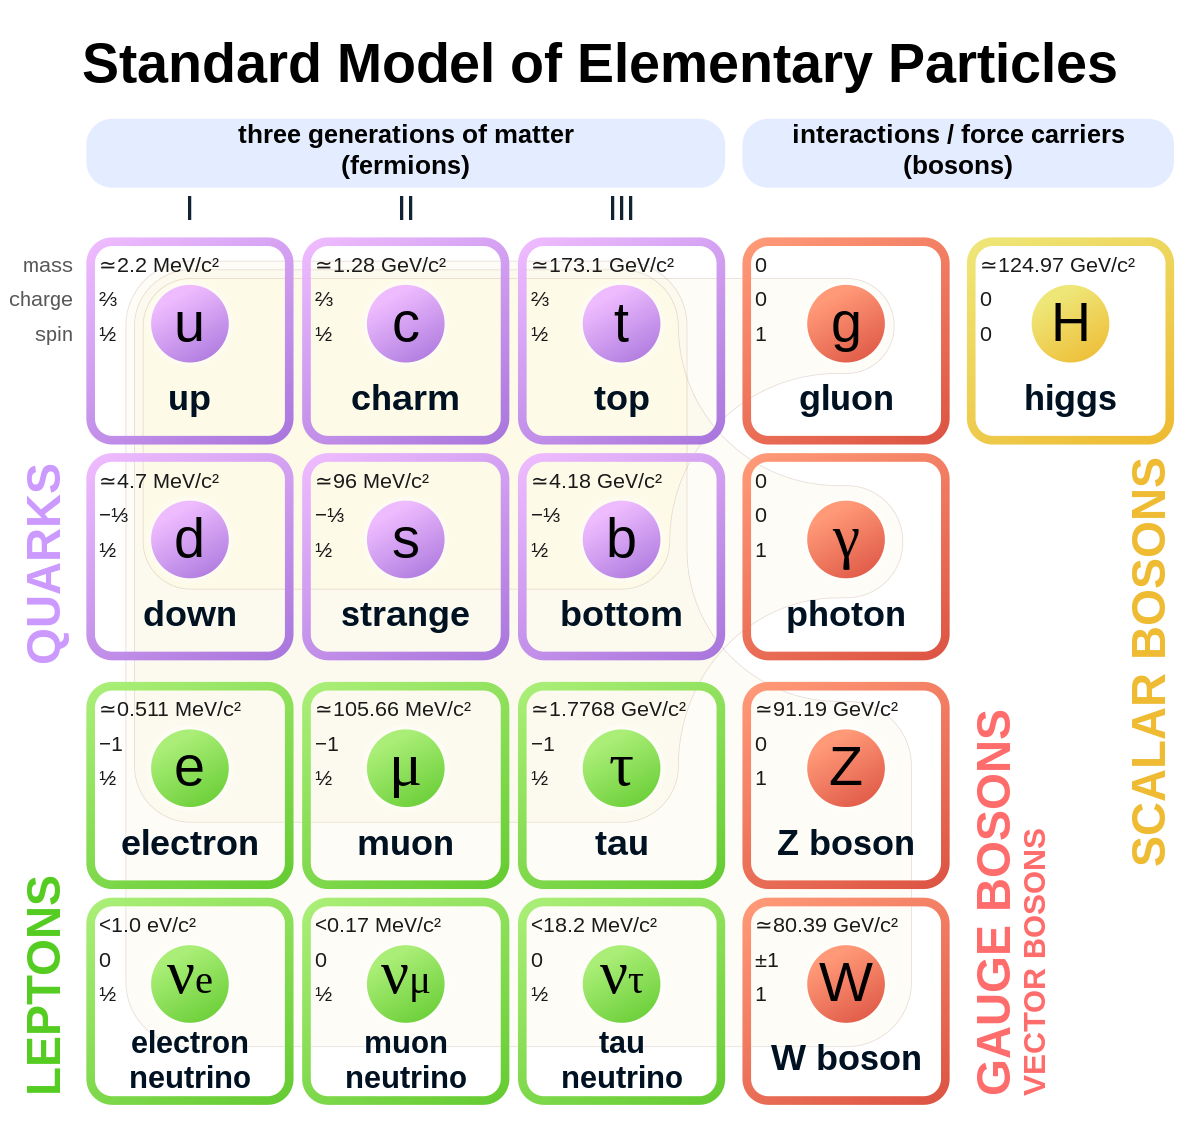
\includegraphics[width=0.5\linewidth]{63_стандартная_модель.png}
    \caption{Частицы стандартной модели}
    \label{fig:стандартная модель}
\end{figure}

\textit{Фундаментальные взаимодействия} -- различные типы взаимодействия между элементарными частицами. Это

\begin{itemize}
    \item \textit{Гравитационное} взаимодействие
    \item \textit{Электромагнитное} взаимодействие
    \item \textit{Сильное} взаимодействие
    \item \textit{Слабое} взаимодействие
\end{itemize}

Состоящие из кварков частицы называются \textit{адронами}. В основном наблюдаются \textit{мезоны} -- частицы, состоящие из двух кварков (кварк + антикварк), и \textit{барионы} -- частицы, состоящие из трёх кварков. Возможные и другие частицы (тетракварки, пентакварки), однако они существуют малое время.

\noindent
Обычных квантовых чисел оказывается недостаточно, чтобы описать кварки. Так, например, существуют частицы, состоящие из трёх кварков в одинаковом состоянии, что невозможно для ферми-частиц. Таким образом существует ещё одно квантовое число -- \textit{цвет} кварков. Адроны в целом \textit{бесцветны}, то есть либо присутствуют все возможные цвета (для барионов) либо цвет и антицвет (для мезонов). Глюонное взаимодействие кварков внутри частицы заключается в <<перекрашивании>> -- переносе цветового заряда между кварками.

Из-за глюонного взаимодействия оказывается невозможным существование свободных кварков. При, например, отдалении одного из кварков нейтрона от других, между ними образуется глюонная трубка, в которой накапливается энергия. При дальнейшем удалении энергии оказывается достаточно для образования новых частиц, что приводит к образованию двух адронов. С другой стороны, при больших энергиях столкновение частиц можно рассматривать как столкновение отдельных кварков друг с другом, поскольку энергия глюонной связи оказывается сравнительно мала.

$W$- и $Z$-бозоны могут осуществлять превращение одних кварков в другие (слабое взаимодействие).


\end{document}